\documentclass[oneside, 12pt]{report}

\usepackage[a4paper, left=3cm, right=3cm, top=4cm, bottom=3cm]{geometry}
\usepackage[T1]{fontenc}
\usepackage[utf8]{inputenc}
\usepackage[italian]{babel}
\usepackage{graphicx}
\graphicspath{{figure/}}
\usepackage{url}
\usepackage[breaklinks, hidelinks]{hyperref}
\usepackage{subfig}
\usepackage{amsmath, amssymb, amsfonts}
\usepackage{braket}         % Notazione di Dirac: \ket{}, \bra{}, \braket{}
\usepackage{textcomp}
\usepackage{xcolor}
\usepackage{afterpage}
\usepackage{bm}
\usepackage{multirow}
\usepackage{algorithm}
\usepackage{algpseudocode}
\usepackage{pgfplots}
\pgfplotsset{compat=1.18}
\usepackage{tikz}
\usetikzlibrary{quantikz2}  % Circuiti quantistici
\usepackage{listings}
\usepackage{microtype}
\usepackage{booktabs}
\usepackage{tabularx}
\usepackage{setspace}
\usepackage[bottom]{footmisc}
\usepackage{float}
\usepackage[backend=biber, citestyle=numeric, sorting=none]{biblatex}
\usepackage[acronym, nopostdot, nogroupskip, toc]{glossaries}
\makenoidxglossaries
% Compatibilità con i comandi del vecchio pacchetto acronym
\let\ac\gls
\providecommand{\acf}[1]{\acrfull{#1}}
\providecommand{\acl}[1]{\acrlong{#1}}
\providecommand{\acs}[1]{\acrshort{#1}}
\begin{acronym}[CRYSTALS]  % larghezza colonna basata sull'acronimo più lungo

    \acro{BHT}{Brassard-H\o yer-Tapp}
    \acro{BQP}{\textit{Bounded-error Quantum Polynomial time}}
    \acro{CCNOT}{Controlled-Controlled NOT (porta di Toffoli)}
    \acro{CDR}{\textit{Clifford Data Regression}}
    \acro{CNF}{Forma Normale Congiuntiva (\textit{Conjunctive Normal Form})}
    \acro{CNOT}{Controlled-NOT}
    \acro{CPTP}{\textit{Completely Positive Trace-Preserving}}
    \acro{DFT}{Trasformata Discreta di Fourier (\textit{Discrete Fourier Transform})}
    \acro{DSA}{\textit{Digital Signature Algorithm}}
    \acro{ECDSA}{\textit{Elliptic Curve Digital Signature Algorithm}}
    \acro{GNFS}{\textit{General Number Field Sieve}}
    \acro{HTTPS}{\textit{HyperText Transfer Protocol Secure}}
    \acro{IBM}{International Business Machines}
    \acro{MIT}{Massachusetts Institute of Technology}
    \acro{NIST}{\textit{National Institute of Standards and Technology}}
    \acro{NISQ}{\textit{Noisy Intermediate-Scale Quantum}}
    \acro{NMR}{Risonanza Magnetica Nucleare (\textit{Nuclear Magnetic Resonance})}
    \acro{PEC}{\textit{Probabilistic Error Cancellation}}
    \acro{PQC}{\textit{Post-Quantum Cryptography}}
    \acro{QEC}{Correzione degli Errori Quantistici (\textit{Quantum Error Correction})}
    \acro{QFT}{Trasformata di Fourier Quantistica (\textit{Quantum Fourier Transform})}
    \acro{QMA}{\textit{Quantum Merlin-Arthur}}
    \acro{QPE}{\textit{Quantum Phase Estimation}}
    \acro{RSA}{Rivest-Shamir-Adleman}
    \acro{SAT}{Soddisfacibilità Booleana (\textit{Boolean Satisfiability})}
    \acro{SSH}{\textit{Secure Shell}}
    \acro{TLS}{\textit{Transport Layer Security}}
    \acro{TSP}{Problema del Commesso Viaggiatore (\textit{Travelling Salesman Problem})}
    \acro{ZNE}{\textit{Zero-Noise Extrapolation}}

\end{acronym}
   % definizioni acronimi nel preambolo

% Stile codice Python/Qiskit
\lstset{
    language=Python,
    basicstyle=\ttfamily\small,
    keywordstyle=\color{blue}\bfseries,
    commentstyle=\color{gray}\itshape,
    stringstyle=\color{orange},
    showstringspaces=false,
    frame=none,
    breaklines=true,
    captionpos=b
}

% Pagina bianca
\newcommand{\blankpage}{%
    \null\thispagestyle{empty}\addtocounter{page}{-1}\newpage
}

\onehalfspacing
\setlength{\skip\footins}{1cm}
\addbibresource{Bibliografia.bib}

\begin{document}

% Frontespizio conforme al modello ufficiale
% "frontspibis ING MAG ISI.doc" (A4, margini laterali 3 cm).
%
% Il modello mette ogni riga in un paragrafo a sé: qui ogni riga è un
% nodo ancorato alla propria linea di base, misurata in mm dal bordo
% superiore della pagina sul PDF esportato dal modello. Così la posizione
% non dipende dall'interlinea del documento (\onehalfspacing).
% Garamond -> EB Garamond; Palatino -> URW Palladio (ppl).
\begin{titlepage}
\thispagestyle{empty}

\begin{tikzpicture}[remember picture, overlay,
    centro/.style={inner sep=0pt, anchor=base},
    sinistra/.style={inner sep=0pt, anchor=base west},
    garamond/.style={font=\fontfamily{EBGaramond-TLF}\fontseries{b}%
        \fontshape{n}\fontsize{#1}{#1}\selectfont},
    garamond corsivo/.style={font=\fontfamily{EBGaramond-TLF}\fontseries{b}%
        \fontshape{it}\fontsize{#1}{#1}\selectfont},
    garamond nome/.style={font=\fontfamily{EBGaramond-TLF}\fontseries{m}%
        \fontshape{it}\fontsize{#1}{#1}\selectfont},
    palatino/.style={font=\usefont{T1}{ppl}{b}{n}\fontsize{#1}{#1}\selectfont},
    palatino nome/.style={font=\usefont{T1}{ppl}{m}{it}\fontsize{#1}{#1}\selectfont}]

    % Matricola: Palatino grassetto 10 pt.
    \node[sinistra, palatino=10]
        at ([shift={(30mm,-28.7mm)}]current page.north west)
        {Matr. N INLM03/23286};

    % Marchio: stessa larghezza d'inchiostro del modello (29,2 mm).
    \node[inner sep=0pt, anchor=north]
        at ([yshift=-35.4mm]current page.north)
        {
\includegraphics[width=30.15mm]{figure/ucbm-logo.png}};

    % Ateneo: Garamond grassetto 16 pt, su due righe.
    \node[centro, garamond=16] at ([yshift=-74.3mm]current page.north)
        {UNIVERSIT\`A};
    \node[centro, garamond=16] at ([yshift=-83.8mm]current page.north)
        {CAMPUS BIO-MEDICO DI ROMA};

    % Facoltà e corso di laurea: Garamond grassetto 14 pt.
    \node[centro, garamond=14] at ([yshift=-112.4mm]current page.north)
        {FACOLT\`A DIPARTIMENTALE DI INGEGNERIA};
    \node[centro, garamond=14] at ([yshift=-118.1mm]current page.north)
        {CORSO DI LAUREA MAGISTRALE IN};
    \node[centro, garamond=14] at ([yshift=-123.6mm]current page.north)
        {INGEGNERIA DEI SISTEMI INTELLIGENTI};

    % Titolo: Garamond grassetto 18 pt, passo di riga del modello (7,13 mm).
    \node[centro, garamond=18] at ([yshift=-151.1mm]current page.north)
        {SHOR'S ALGORITHM UNDER NOISE:};
    \node[centro, garamond=18] at ([yshift=-158.2mm]current page.north)
        {MACHINE-LEARNING ABLATION,};
    \node[centro, garamond=18] at ([yshift=-165.4mm]current page.north)
        {QUANTUM ERROR CORRECTION,};
    \node[centro, garamond=18] at ([yshift=-172.5mm]current page.north)
        {AND APPROXIMATE QFT};

    % Relatore e correlatore: etichetta Garamond grassetto corsivo 14 pt,
    % nome Palatino corsivo 12 pt.
    \node[sinistra, garamond corsivo=14]
        at ([shift={(30mm,-194.2mm)}]current page.north west) {Relatore};
    \node[sinistra, palatino nome=12]
        at ([shift={(30mm,-199.9mm)}]current page.north west) {Prof. Paolo Soda};
    \node[sinistra, garamond corsivo=14]
        at ([shift={(30mm,-224.4mm)}]current page.north west) {Correlatore};
    \node[sinistra, palatino nome=12]
        at ([shift={(30mm,-230.4mm)}]current page.north west) {Ing. Floriano Caprio};

    % Laureando: allineato a sinistra a 142,4 mm dal bordo, dove il modello
    % lo porta con rientro (99,9 + 12,5 mm) e tabulazioni; nome in Garamond.
    \node[sinistra, garamond corsivo=14]
        at ([shift={(142.4mm,-240.5mm)}]current page.north west) {Laureando};
    \node[sinistra, garamond nome=12]
        at ([shift={(142.4mm,-245.6mm)}]current page.north west) {Claudio Dragotta};

    % Anno accademico: Garamond grassetto 12 pt.
    \node[centro, garamond=12] at ([yshift=-275.7mm]current page.north)
        {ANNO ACCADEMICO 2025/2026};
\end{tikzpicture}

\null
\afterpage{\blankpage}
\end{titlepage}


\begin{titlepage}
    \vspace*{5cm}
    \begin{center}
        \emph{Alla mia famiglia, \\
        per il sostegno incondizionato e l'amore che non è mai venuto meno. \\
        A me stesso, per la determinazione e la perseveranza con cui ho affrontato questo percorso.}
    \end{center}
\end{titlepage}

\pagenumbering{roman}
\tableofcontents

% -----------------------------------------------
\addcontentsline{toc}{chapter}{\listfigurename}
\listoffigures

% -----------------------------------------------
\addcontentsline{toc}{chapter}{\listtablename}
\listoftables

% -----------------------------------------------
\printnoidxglossary[type=\acronymtype, nonumberlist, title={Elenco degli Acronimi}]

% -----------------------------------------------
\pagenumbering{arabic}
\chapter{Introduzione}
\label{chap:introduzione}
\begin{onehalfspace}

\section{Il Limite del Calcolo Classico}

Per oltre cinquant'anni, lo sviluppo dell'informatica è stato guidato da una legge empirica enunciata nel 1965 da Gordon Moore\footnote{\textbf{Gordon Earle Moore} (1929--2023), cofondatore di Intel, osservò nel 1965 che il numero di transistor integrabili su un chip raddoppiava approssimativamente ogni due anni, con un conseguente aumento esponenziale delle prestazioni computazionali. La Legge di Moore non è una legge fisica, ma una previsione industriale che ha orientato decenni di investimenti tecnologici.}: il numero di transistor per chip raddoppia ogni due anni, e con esso la potenza di calcolo disponibile. Questa crescita esponenziale ha permesso di trasformare calcolatori grandi quanto un'intera stanza nei dispositivi tascabili di oggi. Tuttavia, la Legge di Moore si sta scontrando con i limiti fisici fondamentali della materia: i transistor moderni hanno dimensioni di pochi nanometri, avvicinandosi alla scala atomica oltre la quale gli effetti quantistici -- lo stesso fenomeno che si vorrebbe evitare -- diventano incontrollabili e inevitabili.

Parallelamente al problema fisico dell'hardware, esiste una barriera di natura puramente matematica: esistono classi di problemi computazionali per i quali nessun algoritmo classico è in grado di fornire una soluzione in tempi ragionevoli, \textit{indipendentemente} dalla potenza di calcolo disponibile. Questi problemi -- fattorizzazione di grandi interi, ricerca in spazi combinatoriali enormi, simulazione di sistemi molecolari complessi -- resistono a qualunque approccio classico non perché i computer non siano abbastanza veloci, ma perché la complessità intrinseca del problema cresce più rapidamente di qualunque risorsa classica concepibile.

È in questo contesto che nasce il \textbf{calcolo quantistico}: la visione radicale che i principi della meccanica quantistica -- \textit{sovrapposizione}, \textit{entanglement} e \textit{interferenza} -- possano essere sfruttati non come ostacoli da evitare, ma come risorse computazionali di straordinaria potenza. L'intuizione originale fu di Richard Feynman\footnote{\textbf{Richard Phillips Feynman} (1918--1988), fisico teorico statunitense, Premio Nobel per la Fisica nel 1965. Nel suo celebre articolo del 1982 \textit{``Simulating Physics with Computers''} \cite{feynman1982}, Feynman argomentò che un computer classico non può simulare efficientemente un sistema quantistico senza un overhead esponenziale, e propose che un ``computer quantistico'' -- uno che segua le leggi della meccanica quantistica -- potrebbe farlo in modo naturalmente efficiente.}, che nel 1982 osservò come la simulazione di sistemi quantistici richiedesse risorse esponenziali su macchine classiche, e propose che un computer basato sugli stessi principi fisici potesse simulare la natura stessa in modo efficiente \cite{feynman1982}. David Deutsch formalizzò nel 1985 il primo modello teorico rigoroso di computer quantistico universale \cite{deutsch1985}, aprendo la strada a un nuovo paradigma computazionale.

\section{La Rivoluzione Algoritmica degli Anni Novanta}

Negli anni successivi alla proposta di Deutsch, la comunità scientifica si interrogò sulla effettiva esistenza di problemi che un computer quantistico potesse risolvere in modo \textit{probabilmente} più efficiente di qualunque macchina classica. La risposta arrivò in forma dirompente nel corso di pochi anni.

Nel 1992, Daniel Simon\footnote{L'\textbf{algoritmo di Simon} (1994, pubblicato nel 1997) fu il primo a dimostrare uno speedup \textit{esponenziale} rispetto a qualunque algoritmo classico probabilistico, stabilendo la prova di principio che i computer quantistici potessero essere genuinamente più potenti. Shor riconobbe che la sua tecnica si ispirava direttamente alle idee di Simon.} identificò un problema artificiale per il quale un algoritmo quantistico era esponenzialmente più veloce di qualunque algoritmo classico. Questo risultato rimase per alcuni anni una curiosità teorica, fino a quando, nel \textbf{1994}, Peter Shor pubblicò un risultato che scosse le fondamenta della sicurezza informatica mondiale: un algoritmo quantistico in grado di fattorizzare un intero di $n$ bit in tempo \textit{polinomiale} $O(n^3)$ \cite{shor1994}, a fronte della complessità sub-esponenziale ma super-polinomiale dei migliori algoritmi classici noti. Le implicazioni furono immediate e devastanti: l'intero edificio della crittografia a chiave pubblica -- \ac{RSA}, Diffie-Hellman, le firme digitali \ac{ECDSA} -- si fondava proprio sull'assunzione che la fattorizzazione fosse computazionalmente intrattabile. Un computer quantistico sufficientemente grande avrebbe reso obsoleta, in un solo colpo, l'intera infrastruttura crittografica su cui poggia Internet.

Due anni dopo, nel \textbf{1996}, Lov Grover presentò un algoritmo di tutt'altra natura, ma di eguale importanza \cite{grover1996}. Mentre Shor aveva risolto un problema specifico della teoria dei numeri, Grover affrontò una sfida universale: la \textbf{ricerca non strutturata}. Dato un insieme di $N$ elementi senza alcuna struttura o ordinamento, trovare quello che soddisfa una certa proprietà richiede, nel caso classico, un numero di interrogazioni proporzionale a $N$. Grover dimostrò che un algoritmo quantistico può fare lo stesso lavoro in sole $O(\sqrt{N})$ interrogazioni -- uno \textit{speedup quadratico} -- e che questo risultato è \textit{ottimale}: nessun algoritmo quantistico può fare di meglio. Sebbene meno spettacolare dello speedup esponenziale di Shor, il vantaggio di Grover è universale, applicabile a qualunque problema di ricerca, e porta con sé implicazioni profonde per la crittografia simmetrica, l'ottimizzazione combinatoria e la ricerca in grandi basi di dati.

Questi due algoritmi -- Shor e Grover -- rappresentano ancora oggi i pilastri dell'informatica algoritmica quantistica: il primo come dimostrazione del potere \textit{esponenziale} del calcolo quantistico su problemi strutturati, il secondo come strumento \textit{universale} di accelerazione quadratica applicabile al problema computazionale più fondamentale.

\section{Lo Stato dell'Arte: dall'Era NISQ ai Computer Fault-Tolerant}

Nonostante la solidità teorica di questi risultati, la realizzazione pratica di computer quantistici di scala sufficiente ad eseguirli su istanze realmente significative incontra ostacoli formidabili. I sistemi quantistici fisici sono intrinsecamente fragili: qualunque interazione non controllata con l'ambiente esterno -- vibrazioni termiche, campi elettromagnetici, imperfezioni nei materiali -- provoca fenomeni di \textbf{decoerenza} -- ossia la perdita progressiva della coerenza quantistica causata dall'entanglement indesiderato tra il qubit e i gradi di libertà ambientali, che sopprime le interferenze quantistiche riducendo il sistema a una miscela statistica classica -- degradando lo stato quantistico in modo irreversibile prima che il calcolo possa completarsi. A differenza di un bit classico, che può essere protetto dalla ridondanza, un qubit non può essere copiato (teorema del no-cloning \cite{wootters1982}) né letto senza distruggerlo: questo rende la correzione degli errori quantistici un problema radicalmente diverso e molto più complesso di quella classica.

Il panorama tecnologico attuale è dominato da un insieme variegato di piattaforme hardware in competizione: \textbf{qubit superconduttori} (\ac{IBM}, Google, Rigetti), \textbf{ioni intrappolati} (IonQ, Quantinuum), \textbf{fotoni} (PsiQuantum, Xanadu) e \textbf{spin in silicio} (Intel). Ciascuna architettura presenta vantaggi e svantaggi in termini di tempi di coerenza, fedeltà delle porte, scalabilità e temperatura operativa.

Un momento simbolico di questa corsa fu raggiunto nel \textbf{2019}, quando il team di Google rivendicò il raggiungimento della cosiddetta \textit{quantum supremacy}\footnote{Il termine \textit{quantum supremacy}, coniato da John Preskill nel 2012, indica il punto in cui un computer quantistico esegue un calcolo specifico in un tempo che nessun supercomputer classico potrebbe eguagliare in modo pratico. La rivendicazione di Google con il processore Sycamore è rimasta controversa: IBM sostenne che il calcolo avrebbe potuto essere eseguito classicamente in 2.5 giorni anziché 10.000 anni, con un algoritmo migliorato. Questo dibattito evidenzia la difficoltà di definire e misurare il vantaggio quantistico.} con il processore Sycamore a 53 qubit \cite{arute2019}: un calcolo specifico fu completato in 200 secondi, mentre le stime attribuivano al più potente supercomputer classico un tempo di circa 10.000 anni per lo stesso compito. Nel 2023, IBM ha presentato il processore \textit{Condor} a 1.121 qubit e ha delineato una roadmap verso sistemi con oltre 100.000 qubit entro la fine del decennio.

Tuttavia, la distanza tra i dispositivi attuali e un computer quantistico \textit{fault-tolerant} -- in grado di eseguire Shor su istanze RSA reali -- è ancora enorme. I processori odierni operano nel regime cosiddetto \ac{NISQ}, un termine coniato da John Preskill nel 2018 \cite{preskill2018} per descrivere macchine con decine o centinaia di qubit fisici, affette da errori significativi che limitano la profondità dei circuiti eseguibili. In questo scenario, la ricerca si concentra su due direzioni parallele e complementari:

\begin{itemize}
    \item \textbf{\ac{QEC}}: tecniche per codificare qubit logici in qubit fisici ridondanti, in modo da rilevare e correggere gli errori durante il calcolo, a costo di un overhead fisico significativo (centinaia o migliaia di qubit fisici per qubit logico);

    \item \textbf{Noise mitigation}: tecniche che, senza richiedere overhead hardware, riducono l'effetto del rumore a livello di post-processing classico, estendendo la portata dei circuiti eseguibili su hardware NISQ.
\end{itemize}

\clearpage

\section{Motivazione e Contributo del Presente Lavoro}

In questo contesto scientifico e tecnologico si inserisce il presente lavoro di tesi. L'algoritmo di Shor rappresenta uno dei risultati più significativi e dirompenti dell'informatica quantistica: la sua capacità di fattorizzare interi in tempo polinomiale minaccia direttamente le fondamenta della crittografia moderna. Tuttavia, la sua esecuzione su hardware NISQ è ostacolata da requisiti stringenti in termini di profondità del circuito, numero di qubit e fedeltà delle porte -- rendendo il rumore quantistico il principale ostacolo alla sua realizzazione pratica.

Questo lavoro si propone di affrontare tale sfida integrando due ambiti in rapida evoluzione: il \textbf{calcolo quantistico} e i \textbf{modelli di intelligenza artificiale}. L'obiettivo centrale è implementare l'algoritmo di Shor su simulatori quantistici realistici, analizzarne sistematicamente la vulnerabilità al rumore nelle sue componenti critiche -- Quantum Fourier Transform, phase estimation e modular exponentiation -- e sviluppare strategie di ottimizzazione e mitigazione basate su modelli di machine learning.

Il contributo originale consiste nella sperimentazione diretta con il framework Qiskit, nella costruzione e analisi di circuiti per l'algoritmo di Shor in presenza di rumore realistico, e nell'applicazione di tecniche di intelligenza artificiale per caratterizzare il rumore, ottimizzare i parametri del circuito e migliorare l'affidabilità dei risultati su hardware NISQ.

L'elaborato si sviluppa seguendo un percorso che va dalle fondamenta teoriche del calcolo quantistico fino ai risultati sperimentali su simulatori rumorosi, fornendo al lettore gli strumenti concettuali e pratici necessari per comprendere sia le potenzialità che i limiti dell'algoritmo di Shor nell'era attuale, e le prospettive aperte dall'integrazione con l'intelligenza artificiale. Gli obiettivi specifici e la struttura dettagliata del lavoro sono descritti nel Capitolo~\ref{chap:obiettivi}.

\end{onehalfspace}


% -----------------------------------------------
\chapter{Obiettivi e Piano Sperimentale}
\label{chap:obiettivi}
\label{chap:specifiche}
\begin{onehalfspace}

Il capitolo traduce la motivazione introduttiva in un contratto sperimentale: definisce ciò che viene verificato, il perimetro entro cui valgono i risultati e le metriche usate. La motivazione crittografica, i requisiti funzionali e la specifica completa di input e output sono riportati nella Sezione~\ref{app:obiettivi} (Sez.~\ref{sec:motivazione}, \ref{sec:requisiti} e~\ref{sec:input_output}).

\section{Obiettivo e Perimetro del Lavoro}

L'obiettivo generale è stabilire quali strategie rendano più affidabile l'esecuzione di Shor in presenza di rumore, distinguendo tre livelli che non sono direttamente intercambiabili: recupero dei candidati dall'istogramma finale, correzione basata sulle sindromi e analisi di sensibilità a un errore logico residuo.

Il lavoro combina tre attività essenziali:
\begin{enumerate}
    \item richiamare il period finding, la \ac{QFT}, la stima di fase e i principali canali di rumore necessari a interpretare gli esperimenti;
    \item implementare e validare Shor, quindi confrontare su simulatori rumorosi la baseline TOP-1, la ricerca TOP-4 e la variante con classificatore, usando gli stessi istogrammi;
    \item costruire una progressione QEC --- ripetizione, Steane $[[7,1,3]]$ e surface code --- e misurare quando la codifica o un decoder appreso riducono l'errore logico. Una successiva analisi applica a Shor un proxy Pauli per gate compilato, senza identificarlo con il tasso di un memory experiment.
\end{enumerate}

Le campagne rumorose complete riguardano l'istanza $N=15$. Le istanze $N=21$ e $N=35$ sono impiegate soltanto per la validazione ideale dell'aritmetica e per l'audit delle risorse: non vengono usate per inferire la scalabilità sotto rumore né per rappresentare una QPU reale.

\section{Domande di Ricerca e Ipotesi}
\label{sec:ipotesi}

La domanda trasversale della prima fase è se il classificatore riduca il numero di iterazioni oltre quanto già ottenibile esaminando più candidati dello stesso istogramma. L'ipotesi principale richiede pertanto un vantaggio di M2 sia rispetto alla baseline M1 sia rispetto all'ablazione TOP-4; F1 e AUC del classificatore sono controlli predittivi secondari, non prove autonome di utilità operativa. Un eventuale vantaggio deve inoltre essere osservabile nei due preset $N=15$, mentre la generalizzazione al crescere di $N$ resta fuori dal perimetro rumoroso.

La progressione sperimentale risponde poi alle seguenti domande:
\begin{description}
    \item[\textbf{DR1.}] Come varia l'output di Shor al crescere dei diversi parametri di rumore, e quali conclusioni sono sostenute dagli sweep controllati?
    \item[\textbf{DR2.}] Come si estrae una sindrome con un codice a ripetizione senza misurare direttamente lo stato logico?
    \item[\textbf{DR3.}] Quali vantaggi e limiti offre Steane $[[7,1,3]]$ nella correzione di un errore Pauli arbitrario?
    \item[\textbf{DR4.}] Il surface code mostra un regime di soglia nel quale aumentare la distanza riduce il logical error rate?
    \item[\textbf{DR5.}] Come varia il successo di Shor sotto un proxy Pauli uniforme per gate e quale beneficio producono ripetizioni indipendenti?
    \item[\textbf{DR6.}] In quale regime un decoder appreso dalla sindrome può migliorare il decoder analitico di riferimento?
\end{description}

Le ipotesi quantitative associate sono: soppressione quadratica dell'errore per i codici di distanza $d=3$ nel regime perturbativo; esistenza di un incrocio delle curve $p_L(p)$ del surface code; andamento non crescente del successo di Shor al crescere del proxy per gate. Per la decodifica appresa il confronto è deliberatamente esplorativo: il modello deve essere valutato sugli stessi campioni e contro \ac{MWPM}, senza presupporne la superiorità.

\section{Contributo e Disegno Sperimentale}
\label{sec:contributo_originale}

Il contributo metodologico è costituito da tre scelte coordinate. Primo, il confronto appaiato M1--TOP-4--M2 separa il valore della ricerca multi-candidato da quello del classificatore. Secondo, la progressione dai codici elementari al surface code usa metriche esplicite e dichiara il confine tra tasso per memoria, tasso per ciclo e proxy per gate. Terzo, il modello appreso viene valutato in due punti diversi della pipeline --- output e sindrome --- così che la sua utilità dipenda dall'informazione effettivamente disponibile, non dalla sola qualità predittiva.

Il protocollo mantiene distinti risultati, validazioni e assunzioni. Circuiti e aritmetica sono prima verificati idealmente; i metodi decisionali ricevono gli stessi campioni; ogni stima riporta seed, numerosità e incertezza; i preset uniformi sono trattati come scenari illustrativi e non come calibrazioni hardware. Il dettaglio implementativo e statistico è nel Capitolo~\ref{chap:metodologia}, mentre gli esperimenti estesi sono raccolti nelle Appendici~\ref{app:fase1} e~\ref{app:fase2}.

\section{Campagne Rumorose e Validazioni Ideali}
\label{sec:use_case}

Il disegno distingue due use case:
\begin{itemize}
    \item \textbf{campagne rumorose N15}: stesso $N=15$, base $a=7$, circuito e budget di shot, con un preset di riferimento e uno di stress;
    \item \textbf{validazioni ideali N21/N35}: verifica dell'aritmetica reversibile, del ripristino delle ancille e della distribuzione QPE, senza simulazione rumorosa completa.
\end{itemize}

\begin{table}[!htbp]
\centering
\small
\begin{tabular}{@{}lcc@{}}
\toprule
\textbf{Parametro} & \textbf{Riferimento} & \textbf{Stress} \\
\midrule
$N$, $a$, periodo atteso $r$ & $15,7,4$ & $15,7,4$ \\
$n_{\mathrm{count}}$ & 8 & 8 \\
$M_{\mathrm{shots}}$ & 1024 & 1024 \\
$\epsilon_{1q}=\lambda_{1q}$ & $1\times10^{-3}$ & $5\times10^{-3}$ \\
$\epsilon_{2q}=\lambda_{2q}$ & $1\times10^{-2}$ & $5\times10^{-2}$ \\
$T_1$ (ns) & 100\,000 & 50\,000 \\
$T_2$ (ns) & 80\,000 & 30\,000 \\
$p_{\mathrm{ro}}$ & $2\times10^{-2}$ & $5\times10^{-2}$ \\
\bottomrule
\end{tabular}
\caption{Preset uniformi delle campagne rumorose N15; non rappresentano la calibrazione di una QPU.}
\label{tab:use_case_params}
\end{table}

I parametri $\lambda_{1q}$ e $\lambda_{2q}$ sono quelli passati al canale depolarizzante di Aer; il readout è modellato mediante una matrice di confusione simmetrica. Il modello è uniforme e non comprende topologia, routing, crosstalk o deriva temporale.

\subsection{Razionale per la Scelta delle Istanze}
\label{subsec:razionale_istanze}

Per $N=15$, la base $a=7$ ha periodo atteso $r=4$ e consente un circuito abbastanza contenuto da sostenere confronti appaiati e sweep. Per $N=21$, $a=2$, e $N=35$, $a=6$, l'aritmetica di Beauregard è invece validata idealmente sui vettori di base e mediante QPE. La separazione evita di trasformare un limite computazionale del simulatore in un'affermazione sul successo dell'algoritmo.

\section{Metriche di Valutazione}
\label{sec:metriche}

\subsection{Post-processing dell'Output}

M1 usa il solo candidato più frequente; $M_{\mathrm{TOP4}}$ verifica i quattro candidati dominanti; M2 applica il classificatore prima della stessa ricerca TOP-4. Per ciascun metodo $j$ si riportano il numero medio di iterazioni $\bar M_j$, la dispersione e la probabilità di successo entro il budget preregistrato $M_{\max}=50$. Il confronto descrittivo tra baseline e metodo con classificatore usa
\begin{equation}
    \rho=\frac{\bar M_1}{\bar M_2},
    \label{eq:ipotesi_rho}
\end{equation}
mentre l'ablazione richiede il confronto separato con $M_{\mathrm{TOP4}}$. Un valore $\rho>1$ indica soltanto una media inferiore per M2: l'inferenza è condotta sulle differenze appaiate complete. I fallimenti sono conservati mediante una sentinella oltre il budget; test, gestione degli zeri e tie-break deterministico sono specificati nel Capitolo~\ref{chap:metodologia}. F1 e AUC descrivono il classificatore, ma non sostituiscono la metrica operativa.

\subsection{Correzione d'Errore}
\label{subsec:metriche_qec}

La metrica centrale è il \textbf{logical error rate} $p_L$, stimato con intervallo di confidenza in funzione dell'errore fisico $p$ e della distanza $d$. La pendenza $\gamma$ in $p_L\propto p^\gamma$ verifica la soppressione a basso errore; il \emph{break-even} è il regime $p_L<p$; la soglia $p_{th}$ è individuata dall'incrocio delle curve a distanze diverse. Per l'analisi di Shor si misurano inoltre la probabilità per singola esecuzione e quella cumulativa $P(k)=1-(1-P_s)^k$.

Il simbolo $p_L$ compare in due contesti che restano distinti: nei benchmark QEC è un tasso riferito allo specifico circuito di memoria o correzione; nel proxy di Shor è la probabilità di un Pauli non identità dopo ciascun gate compilato incluso nel modello. Una conversione tra i due richiederebbe una compilazione fault-tolerant per operazione e non viene assunta.

\section{Approccio Metodologico}

La trattazione procede dalla teoria alla verifica ideale, quindi alle campagne appaiate e alla QEC. Architettura software, modelli di rumore, protocolli statistici e implementazione dei metodi sono descritti nel Capitolo~\ref{chap:metodologia}; questo capitolo ne fissa soltanto obiettivi, perimetro e criteri di valutazione.

\end{onehalfspace}


% -----------------------------------------------
\chapter{Fondamenti del Calcolo Quantistico}
\label{chap:fondamenti}
\begin{onehalfspace}

Questo capitolo introduce l'algoritmo che dà a questa tesi il proprio oggetto. Si apre con i richiami di calcolo quantistico indispensabili a seguirlo --- il qubit, la sovrapposizione, le porte unitarie e il meccanismo di interferenza --- di cui l'algoritmo costituisce l'applicazione più celebre.

L'\textbf{algoritmo di Shor}, proposto da Peter Shor nel 1994 \cite{shor1994}, è un algoritmo quantistico che risolve il problema della \textbf{fattorizzazione intera} di un numero $N$ in tempo \textbf{polinomiale} nel numero di bit di $N$:
\begin{equation}
    T_{\text{Shor}}(N) = O\!\left((\log N)^3\right)
    \label{eq:shor_complexity}
\end{equation}

Questo risultato costituisce uno \textbf{speedup esponenziale} rispetto al miglior algoritmo classico noto -- il \ac{GNFS} -- che richiede tempo sub-esponenziale (si veda l'equazione~\eqref{eq:gnfs_complexity}), del tutto impraticabile per i numeri di grandi dimensioni usati in crittografia. È considerato il risultato algoritmico più dirompente dell'informatica quantistica, poiché la fattorizzazione è il fondamento matematico del sistema crittografico RSA, che protegge la quasi totalità delle comunicazioni digitali moderne.

L'algoritmo si articola in tre fasi: un \textit{preprocessing} classico che riconduce il problema a trovare il periodo di una funzione modulare; un nucleo quantistico basato sulla \ac{QFT} e sulla \ac{QPE}, che trova quel periodo in modo esponenzialmente più efficiente di qualunque strategia classica; e una \textit{post-elaborazione} classica che estrae i fattori di $N$ tramite il calcolo del massimo comune divisore. Dopo i richiami si introduce il problema che l'algoritmo risolve e la sua rilevanza crittografica, per poi svilupparne nel dettaglio la struttura.

\section{Richiami di Calcolo Quantistico}
\label{chap:fondamenti}

Questa sezione richiama i concetti di meccanica quantistica e di calcolo quantistico necessari a seguire il resto della tesi, riportando per esteso quelli su cui i capitoli successivi si appoggiano operativamente --- la sfera di Bloch, le matrici di Pauli e la loro algebra. La trattazione completa, con i quattro postulati, l'insieme esteso delle porte e il modello di complessità, è nella Sezione~\ref{app:fondamenti}.

\subsection{Qubit, Sovrapposizione e Sfera di Bloch}

L'unità fondamentale del calcolo quantistico è il \textbf{qubit}, descritto da un vettore unitario nello spazio di Hilbert $\mathcal{H} = \mathbb{C}^2$. In notazione di Dirac, lo stato generico è la \textbf{sovrapposizione}
\begin{equation}
    \ket{\psi} = \alpha\ket{0} + \beta\ket{1}, \qquad \alpha, \beta \in \mathbb{C}, \quad |\alpha|^2 + |\beta|^2 = 1,
\end{equation}
dove $|\alpha|^2$ e $|\beta|^2$ sono le probabilità di misurare rispettivamente $0$ e $1$ (\textbf{regola di Born}).

Riparametrizzando le due ampiezze complesse tramite angoli reali --- il che è lecito perché la normalizzazione toglie un grado di libertà e la fase globale è inosservabile --- ogni stato puro si scrive
\begin{equation}
    \ket{\psi} = \cos\!\left(\frac{\theta}{2}\right)\ket{0} + e^{i\phi}\sin\!\left(\frac{\theta}{2}\right)\ket{1},
    \qquad \theta \in [0,\pi],\ \phi \in [0,2\pi),
    \label{eq:bloch_param}
\end{equation}
e si visualizza come un punto sulla superficie della \textbf{sfera di Bloch}.\footnote{La sfera deve il nome al fisico svizzero-americano Felix Bloch (1905--1983), Premio Nobel per la Fisica nel 1952 per lo sviluppo della spettroscopia a risonanza magnetica nucleare (\ac{NMR}). La stessa notazione $T_1$ e $T_2$ per i tempi di decoerenza proviene dal formalismo NMR di Bloch.} I poli sono $\ket{0}$ e $\ket{1}$, l'equatore le sovrapposizioni equiprobabili con fasi diverse.

\begin{figure}[H]
    \centering
    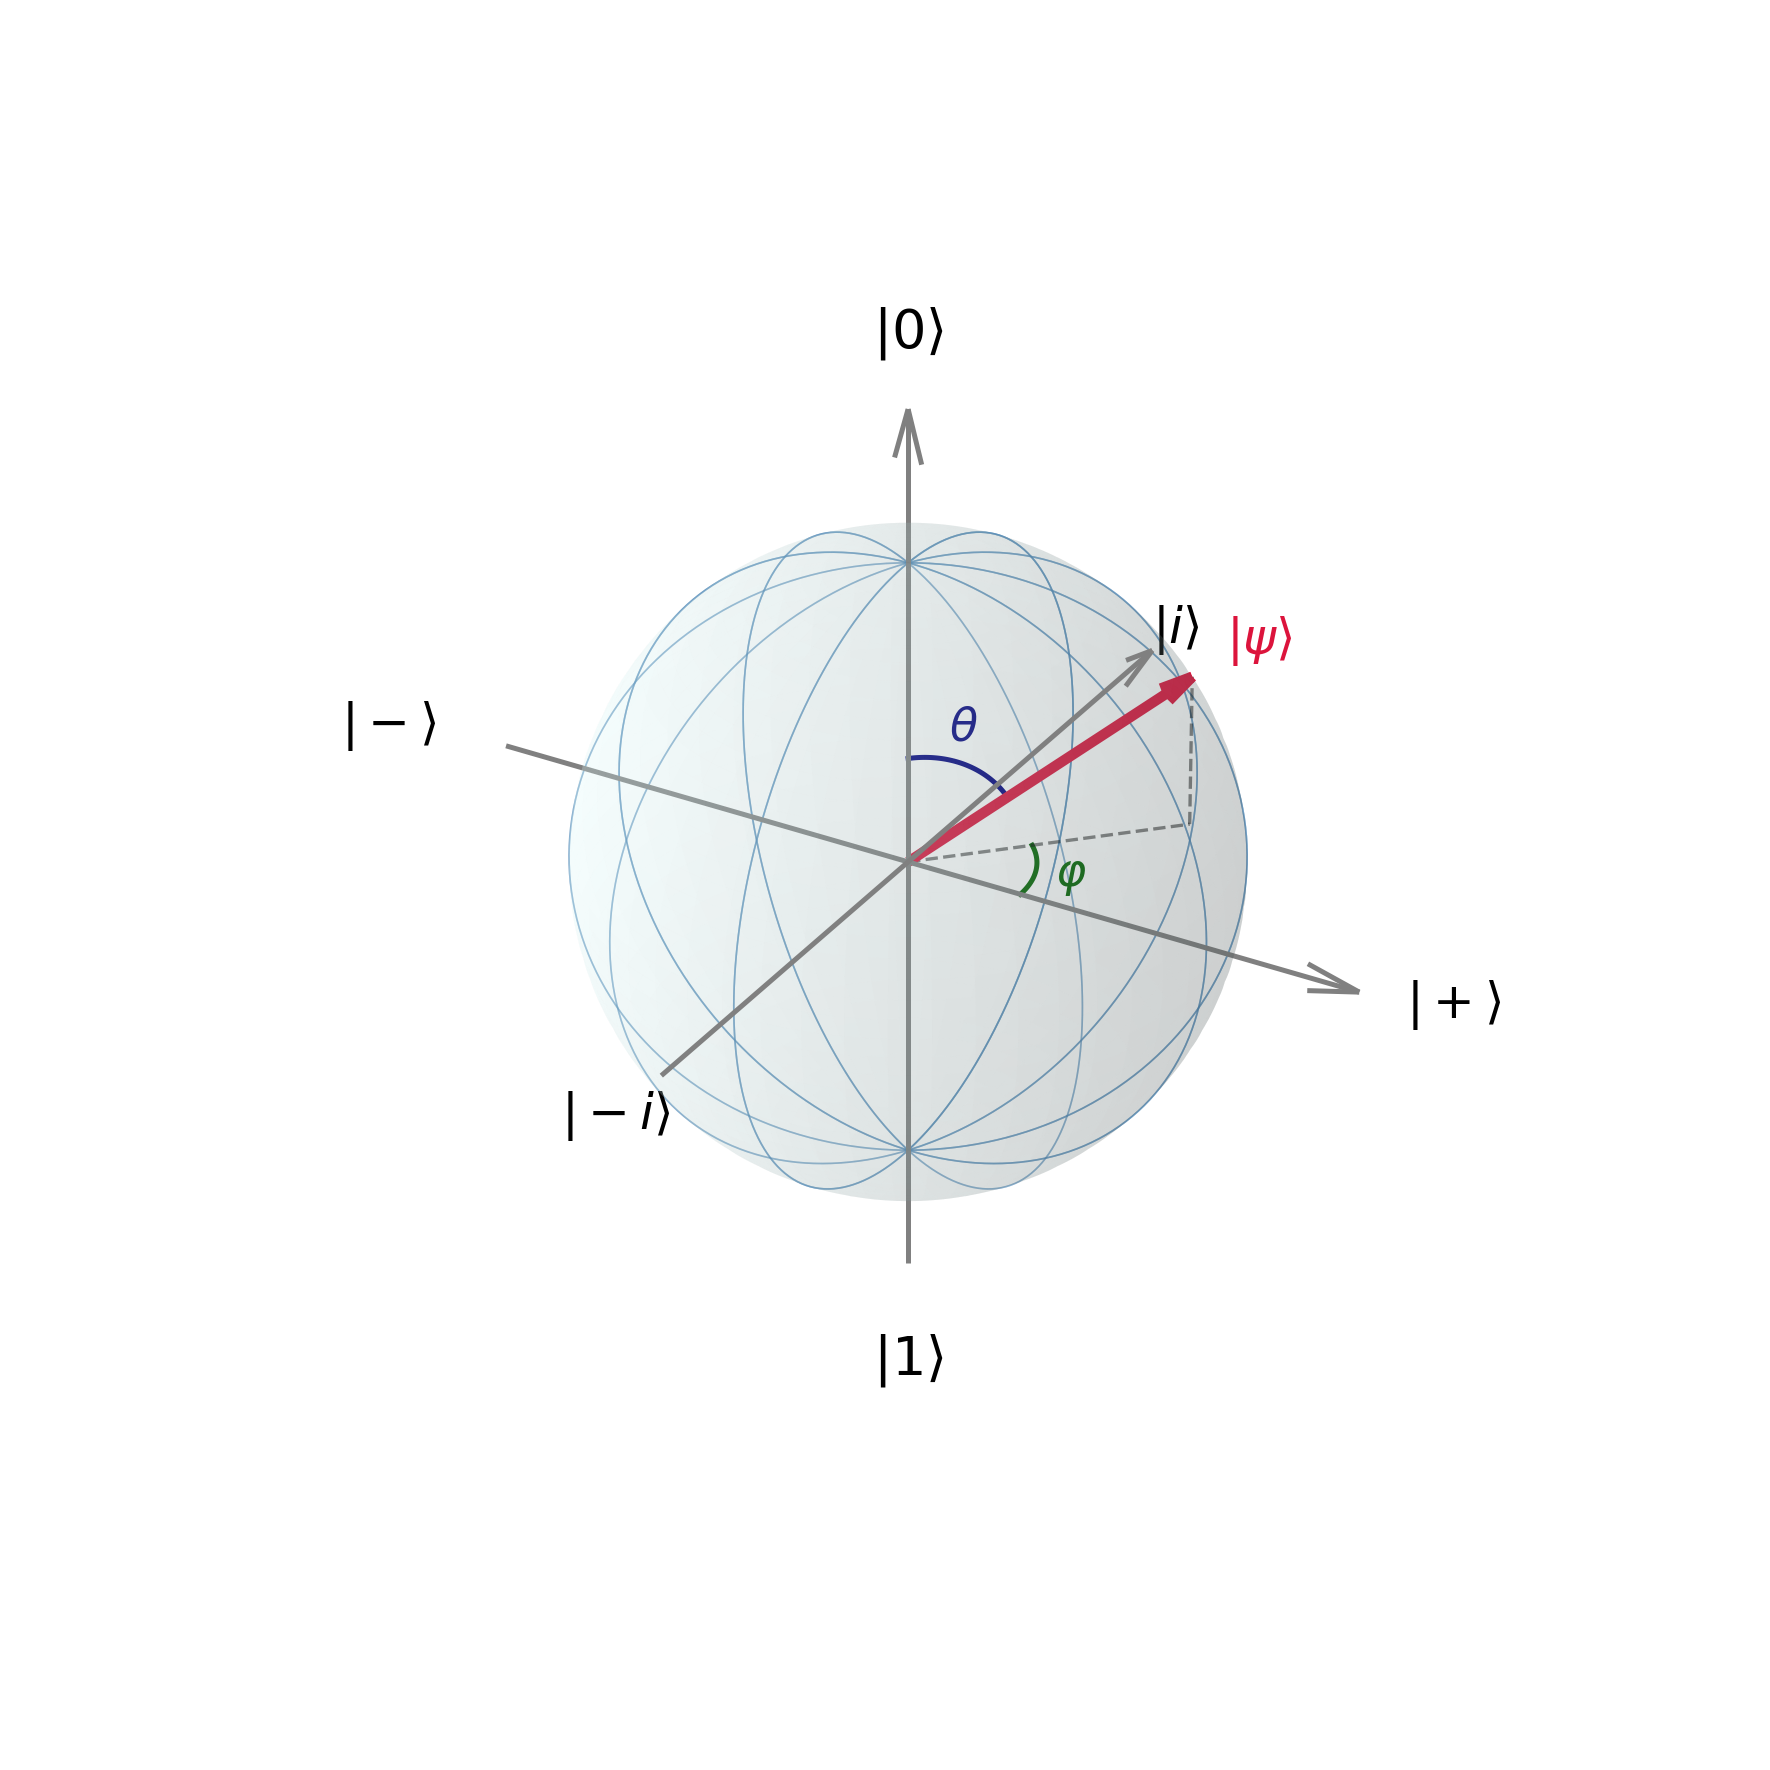
\includegraphics[width=0.42\textwidth]{bloch_sphere.png}
    \caption[La sfera di Bloch]{La sfera di Bloch: ogni stato puro di un qubit corrisponde a un punto sulla superficie della sfera unitaria, parametrizzato dagli angoli $\theta$ e $\varphi$ della~\eqref{eq:bloch_param}. I poli nord e sud rappresentano gli stati base $\ket{0}$ e $\ket{1}$; i punti sull'equatore corrispondono a sovrapposizioni equiprobabili. È la rappresentazione a cui si farà riferimento nel Capitolo~\ref{chap:rumore} per descrivere l'azione dei canali di rumore, che deformano la sfera anziché spostare punti su di essa.}
    \label{fig:bloch}
\end{figure}

\subsection{Sistemi Multi-Qubit ed Entanglement}

Un registro di $n$ qubit vive nello spazio $\mathbb{C}^{2^n}$, ottenuto per \textbf{prodotto tensoriale}. La dimensione esponenziale rende possibile rappresentare ampiezze e correlazioni non disponibili a un registro classico di $n$ bit, ma non implica da sola un vantaggio computazionale: alcune famiglie di stati e circuiti quantistici ammettono infatti descrizioni classiche efficienti. Due qubit sono \textbf{entangled} quando il loro stato congiunto non è fattorizzabile nel prodotto degli stati individuali; l'esempio canonico è lo stato di Bell $\ket{\Phi^+} = \tfrac{1}{\sqrt{2}}(\ket{00} + \ket{11})$, per il quale misure nella stessa base producono esiti perfettamente correlati, senza consentire comunicazione istantanea.

\subsubsection{L'Entanglement come Risorsa Fisica Fragile}

L'entanglement è una risorsa importante per Shor: durante l'esponenziazione modulare il registro di controllo si correla con quello di lavoro, permettendo alla successiva Quantum Fourier Transform di rendere osservabile la periodicità. Un qubit reale, però, non è perfettamente isolato: l'accoppiamento con l'ambiente riduce le coerenze dello stato --- la \textbf{decoerenza}~\cite{zurek2003}. Il tempo caratteristico della perdita di fase è $T_2$ (\textit{dephasing time}); nei dispositivi superconduttori è spesso dello stesso ordine di poche centinaia di durate di una porta a due qubit. Questo confronto segnala un budget di profondità severo, ma non determina una soglia universale nella dimensione di $N$: compilazione, parallelismo, tempi di idle, qualità dei gate e architettura fault-tolerant concorrono tutti al limite discusso nel Capitolo~\ref{chap:rumore}.

\subsection{Porte, Misura e Interferenza}

Le operazioni sui qubit sono \textbf{matrici unitarie} ($U^\dagger U = I$), quindi reversibili. La Tabella~\ref{tab:porte_essenziali} raccoglie quelle su cui il resto della tesi si appoggia; l'insieme completo, con le derivazioni, è nella Sezione~\ref{app:fondamenti}.

\begin{table}[H]
\centering
\begin{tabular}{llc l}
\toprule
\textbf{Porta} & \textbf{Matrice} & \textbf{Qubit} & \textbf{Effetto} \\
\midrule
$X$ & $\begin{pmatrix} 0 & 1 \\ 1 & 0 \end{pmatrix}$ & 1 & \textit{bit flip}: scambia $\ket{0}$ e $\ket{1}$ \\[10pt]
$Y$ & $\begin{pmatrix} 0 & -i \\ i & 0 \end{pmatrix}$ & 1 & bit flip e phase flip insieme ($\propto XZ$) \\[10pt]
$Z$ & $\begin{pmatrix} 1 & 0 \\ 0 & -1 \end{pmatrix}$ & 1 & \textit{phase flip}: $\ket{1} \mapsto -\ket{1}$ \\[10pt]
$H$ & $\tfrac{1}{\sqrt{2}}\begin{pmatrix} 1 & 1 \\ 1 & -1 \end{pmatrix}$ & 1 & genera la sovrapposizione uniforme \\[10pt]
$R_\phi$ & $\begin{pmatrix} 1 & 0 \\ 0 & e^{i\phi} \end{pmatrix}$ & 1 & rotazione di fase; $T = R_{\pi/4}$, $S = R_{\pi/2}$ \\[10pt]
CNOT & $\begin{pmatrix} 1&0&0&0 \\ 0&1&0&0 \\ 0&0&0&1 \\ 0&0&1&0 \end{pmatrix}$ & 2 & nega il \textit{target} se il \textit{control} è $\ket{1}$ \\
\bottomrule
\end{tabular}
\caption[Le porte quantistiche essenziali]{Le porte su cui poggia il resto dell'elaborato. Le tre matrici di Pauli descrivono i canali di rumore del Capitolo~\ref{chap:rumore} e gli errori che i codici correttori dei Capitoli~\ref{chap:qec}--\ref{chap:surface} devono diagnosticare; $H$ e $R_\phi$ costruiscono la \ac{QFT}; la \ac{CNOT} è la porta a due qubit dominante nel conteggio delle risorse, ed è quella a cui è associato l'errore più severo.}
\label{tab:porte_essenziali}
\end{table}

L'identità e le tre matrici di Pauli formano una base dello spazio degli operatori lineari $2\times2$: ogni operatore d'errore su un singolo qubit si può quindi decomporre in tale base. Poiché $Y=iXZ$, un codice che soddisfa le condizioni di correzione per gli errori di Pauli singoli corregge, per linearità, anche le loro combinazioni --- proprietà su cui si fonda l'intera parte \ac{QEC}. Valgono inoltre le relazioni
\begin{equation}
\begin{aligned}
    X^2 = Y^2 = Z^2 &= I, \\
    XY = iZ, \quad YZ = iX, \quad ZX &= iY, \\
    \{X,Y\} = \{Y,Z\} = \{X,Z\} &= 0,
\end{aligned}
    \label{eq:algebra_pauli}
\end{equation}
dove $\{A,B\} = AB+BA$ è l'anticommutatore. Nella teoria degli stabilizzatori, un errore è rilevato quando anticommuta con almeno uno dei generatori misurati; è il vettore completo di questi esiti di commutazione a costituire la sindrome. Nei codici \ac{CSS}, le famiglie di stabilizzatori $X$ e $Z$ permettono di diagnosticare separatamente le due componenti di Pauli, come discusso nel Capitolo~\ref{chap:qec}.

Insieme alle porte a singolo qubit, la \ac{CNOT} forma un insieme universale: ogni operazione unitaria su $n$ qubit si approssima a piacere componendo elementi di questo insieme. La \textbf{misura} in base computazionale collassa lo stato $\ket{\psi}=\sum_x\alpha_x\ket{x}$ sull'esito $x$ con probabilità $|\alpha_x|^2$: è un'operazione non unitaria e irreversibile. Il meccanismo che rende utile tutto ciò è l'\textbf{interferenza}: un algoritmo efficiente è costruito perché le ampiezze degli esiti sbagliati si cancellino (interferenza distruttiva) e quelle degli esiti corretti si sommino (costruttiva). È esattamente ciò che la QFT realizza nell'algoritmo di Shor (Capitolo~\ref{chap:shor}) per far emergere il periodo.

\end{onehalfspace}


% -----------------------------------------------
\chapter{L'Algoritmo di Shor}
\label{chap:shor}
\begin{onehalfspace}

\section{Il Problema della Fattorizzazione Intera}

La \textbf{fattorizzazione intera} consiste nel trovare i fattori primi di un numero intero $N$. Per numeri piccoli il problema è banale, ma la sua difficoltà cresce in modo impressionante all'aumentare di $N$: i migliori algoritmi classici noti, come il \textit{General Number Field Sieve} (\ac{GNFS}), richiedono un tempo sub-esponenziale ma comunque super-polinomiale:\footnote{Il \ac{GNFS} detiene il record mondiale per la fattorizzazione classica: nel 2020, un consorzio internazionale ha fattorizzato RSA-250 (829 bit, 250 cifre decimali) \cite{rsa250_2020}, impiegando l'equivalente di circa 2700 anni-core. In precedenza, nel 2009, era stato fattorizzato RSA-768 (768 bit). I numeri RSA usati in produzione sono di 2048 o 4096 bit, rendendo la fattorizzazione classica del tutto impraticabile con qualunque tecnologia convenzionale prevedibile.}
\begin{equation}
    T_{\text{classico}}(N) = O\!\left(\exp\!\left(c(\log N)^{1/3}(\log\log N)^{2/3}\right)\right)
\end{equation}

Questo problema è classificato in NP ma non è noto se appartenga a P: non esiste alcun algoritmo classico polinomiale per risolverlo, e si congettura fortemente che non esista.

\subsection{Rilevanza Crittografica: RSA}

Il sistema crittografico \textbf{RSA} (Rivest-Shamir-Adleman, 1977) \cite{rsa1978} è il più diffuso algoritmo a chiave pubblica, alla base di HTTPS, TLS, SSH e di gran parte delle comunicazioni digitali sicure. La sua sicurezza si fonda interamente sulla difficoltà computazionale della fattorizzazione:

\begin{itemize}
    \item Si scelgono due grandi primi $p$ e $q$ (tipicamente 1024--4096 bit ciascuno);
    \item Si calcola il modulo $N = p \cdot q$ (la \textit{chiave pubblica} include $N$ ed un esponente $e$);
    \item La \textit{chiave privata} è determinata da $d$ tale che $ed \equiv 1 \pmod{\lambda(N)}$, dove $\lambda$ è la funzione di Carmichael;
    \item Decifrare un messaggio senza conoscere $p$ e $q$ equivale, in pratica, a fattorizzare $N$.
\end{itemize}

Fattorizzare un numero RSA a 2048 bit richiederebbe, con gli algoritmi classici attuali, un tempo stimato superiore all'età dell'universo. Nel 1994, Peter Shor\footnote{\textbf{Peter Williston Shor} (nato nel 1959 a New York) è professore di matematica applicata al \ac{MIT}. Al momento della scoperta dell'algoritmo lavorava presso i laboratori di ricerca AT\&T Bell Labs. Il suo algoritmo è considerato la dimostrazione più impattante del potere del calcolo quantistico.} dimostrò che un computer quantistico può eseguire questa fattorizzazione in tempo \textit{polinomiale}, rendendo RSA teoricamente vulnerabile \cite{shor1994}.

\section{Riduzione alla Ricerca del Periodo}

L'intuizione geniale di Shor consiste nel ricondurre la fattorizzazione a un problema di \textbf{period finding}, trattabile quantisticamente in modo efficiente.

\begin{description}
    \item[Osservazione chiave:] Dato $N$ e un intero $a$ con $\gcd(a, N) = 1$ (coprimo con $N$), la funzione
    \begin{equation}
        f(x) = a^x \bmod N
    \end{equation}
    è \textbf{periodica} con periodo $r$ (detto \textit{ordine} di $a$ modulo $N$): $f(x+r) = f(x)$ per ogni $x$.
\end{description}

Una volta trovato il periodo $r$, se $r$ è pari si può calcolare:
\begin{equation}
    \gcd\!\left(a^{r/2} - 1, N\right) \quad \text{e} \quad \gcd\!\left(a^{r/2} + 1, N\right)
\end{equation}

Con alta probabilità, almeno uno di questi due valori è un fattore non banale di $N$. La prova utilizza proprietà della teoria dei numeri: in particolare, vale $(a^{r/2}-1)(a^{r/2}+1) = a^r - 1 \equiv 0 \pmod{N}$.

\section{La Quantum Fourier Transform}

Il componente quantistico fondamentale dell'algoritmo di Shor è la \textbf{Quantum Fourier Transform} (QFT), l'analogo quantistico della Trasformata Discreta di Fourier (DFT).

\subsection{Definizione}

La QFT su $\mathbb{Z}_{2^n}$ agisce su uno stato base come:
\begin{equation}
    \text{QFT}\ket{j} = \frac{1}{\sqrt{2^n}} \sum_{k=0}^{2^n-1} e^{2\pi i jk / 2^n} \ket{k}
\end{equation}

L'azione su uno stato generico $\ket{\psi} = \sum_j \alpha_j \ket{j}$ produce:
\begin{equation}
    \text{QFT}\ket{\psi} = \sum_k \hat{\alpha}_k \ket{k}
\end{equation}

dove $\hat{\alpha}_k = \frac{1}{\sqrt{2^n}}\sum_j \alpha_j e^{2\pi i jk/2^n}$ sono i coefficienti della DFT.

\subsection{Implementazione Efficiente}

La DFT classica su $N = 2^n$ elementi richiede $O(N \log N)$ operazioni (con il Fast Fourier Transform). La QFT, invece, richiede solo $O(n^2) = O((\log N)^2)$ porte quantistiche, ottenendo uno speedup esponenziale.

Il circuito della QFT è costruito ricorsivamente tramite porte di Hadamard e porte di fase controllate $CR_k$ dove:
\begin{equation}
    CR_k = \begin{pmatrix} 1&0&0&0\\0&1&0&0\\0&0&1&0\\0&0&0&e^{2\pi i/2^k} \end{pmatrix}
\end{equation}

\subsection{Phase Estimation}

La QFT è impiegata, all'interno dell'algoritmo di Shor, attraverso la subroutine di \textbf{Phase Estimation} (QPE). Data una porta $U$ con autovettore $\ket{u}$ e autovalore $e^{2\pi i \theta}$, la QPE stima $\theta$ con precisione arbitraria in tempo $O(n^2)$. Nell'algoritmo di Shor, $U$ è l'operatore di moltiplicazione modulare $U\ket{x} = \ket{ax \bmod N}$, e il suo spettro di fase contiene l'informazione sul periodo $r$.

\section{L'Algoritmo di Shor: Schema Completo}

\begin{algorithm}[H]
\caption{Algoritmo di Shor per la fattorizzazione di $N$}
\begin{algorithmic}[1]
\Require Numero composto $N$, numero di qubit $n = 2\lceil\log_2 N\rceil$
\Ensure Fattore non banale di $N$, oppure \textit{fallimento}
\State Scegliere $a \in \{2, \ldots, N-1\}$ casuale
\State Se $g = \gcd(a,N) > 1$ allora \Return $g$ \Comment{Fortuna: $a$ già condivide un fattore}
\State Inizializzare $\ket{0}^{\otimes n}\ket{1}$
\State Applicare $H^{\otimes n}$ al primo registro: $\frac{1}{\sqrt{2^n}}\sum_{x=0}^{2^n-1}\ket{x}\ket{1}$
\State Applicare l'oracolo di moltiplicazione modulare: $\frac{1}{\sqrt{2^n}}\sum_{x=0}^{2^n-1}\ket{x}\ket{a^x \bmod N}$
\State Misurare il secondo registro: il primo collassa in sovrapposizione degli $x$ con stesso residuo
\State Applicare la QFT inversa al primo registro
\State Misurare il primo registro: ottenere una stima di $s/r$
\State Usare l'algoritmo delle frazioni continue per determinare $r$ da $s/r$
\If{$r$ è dispari o $a^{r/2} \equiv -1 \pmod{N}$} \Return \textit{Fallimento}
\Else
    \State Calcolare $p = \gcd(a^{r/2}-1, N)$ e $q = \gcd(a^{r/2}+1, N)$
    \If{$p$ o $q$ è un fattore non banale di $N$} \Return $p$ o $q$
    \EndIf
\EndIf
\end{algorithmic}
\end{algorithm}

\section{Analisi della Complessità}

La complessità dell'algoritmo di Shor è \textbf{polinomiale} nel numero di bit di $N$:
\begin{itemize}
    \item Il circuito quantistico richiede $O((\log N)^2 \log\log N)$ porte elementari;
    \item Il numero di qubit necessari è $O(\log N)$;
    \item Il numero atteso di iterazioni (con basi $a$ diverse) prima del successo è $O(1)$.
\end{itemize}

Complessivamente: $T_{\text{Shor}}(N) = O\!\left((\log N)^3\right)$, a fronte del $O(\exp((\log N)^{1/3}))$ del miglior algoritmo classico. Si tratta di uno \textbf{speedup esponenziale}.

\section{Impatto sulla Crittografia e Prospettive Post-Quantum}

L'algoritmo di Shor rende teoricamente vulnerabili tutti i sistemi crittografici basati sulla difficoltà della fattorizzazione (RSA) o del logaritmo discreto (Diffie-Hellman, DSA, ECDSA). La \textit{Post-Quantum Cryptography} (PQC) è il campo emergente che sviluppa algoritmi crittografici resistenti agli attacchi quantistici.

Il processo di standardizzazione \ac{PQC} del \ac{NIST}, avviato nel 2016 con una call pubblica per la raccolta di proposte algoritmiche, si è concluso con la pubblicazione formale dei primi standard federali nell'agosto 2024 \cite{nist2024pqc}:\footnote{Dopo otto anni di valutazione e quattro round di selezione pubblica con la partecipazione di crittografi di tutto il mondo, il NIST ha pubblicato nel 2024 i FIPS 203, 204 e 205. Un quarto standard, FIPS 206 (FN-DSA, basato su FALCON), è in fase di finalizzazione. I nuovi nomi riflettono le famiglie algoritmiche di appartenenza: ML-KEM (Module-Lattice Key Encapsulation), ML-DSA (Module-Lattice Digital Signature), SLH-DSA (Stateless Hash-based Digital Signature).}
\begin{itemize}
    \item \textbf{FIPS 203 -- ML-KEM} (basato su CRYSTALS-Kyber): standard per l'incapsulamento di chiave, basato su reticoli modulari;
    \item \textbf{FIPS 204 -- ML-DSA} (basato su CRYSTALS-Dilithium): standard per la firma digitale su reticoli;
    \item \textbf{FIPS 205 -- SLH-DSA} (basato su SPHINCS+): standard per la firma digitale basata su funzioni hash;
    \item \textbf{FIPS 206 -- FN-DSA} (basato su FALCON): standard in fase di finalizzazione per la firma digitale su reticoli NTRU.
\end{itemize}

Questi sistemi si basano su problemi matematici (reticoli, hash, codici) per i quali non sono noti algoritmi quantistici efficienti, garantendo sicurezza anche nell'era post-quantum. La transizione verso questi standard è urgente anche per il cosiddetto fenomeno \textit{harvest now, decrypt later}: attori malevoli raccolgono oggi comunicazioni cifrate con RSA, con l'intenzione di decifrarle quando saranno disponibili computer quantistici fault-tolerant.

\section{Sviluppi Recenti e Stato dell'Arte}

\subsection{Implementazioni su Hardware Reale}

Nonostante la solidità teorica, l'esecuzione di Shor su hardware reale rimane limitata a istanze molto piccole a causa dei requisiti di profondità circuitale. I principali risultati sperimentali sono:

\begin{itemize}
    \item \textbf{2001 -- NMR (Vandersypen et al.)}: prima dimostrazione sperimentale di Shor su un sistema a 7 spin nucleari; fattorizzazione di $N = 15$ in $3 \times 5$ \cite{vandersypen2001}.
    \item \textbf{2016 -- Ioni intrappolati (Monz et al.)}: implementazione scalabile su 5 qubit ionici; fattorizzazione di $N = 15$ con un'architettura modulare \cite{monz2016}.
    \item \textbf{2021 -- Qubit superconduttori IBM}: dimostrazione della fattorizzazione di $N = 21$ su processori IBM Quantum utilizzando solo 5 qubit \cite{skosana2021}, attualmente il risultato più avanzato su hardware superconduttore di uso generale;
    \item \textbf{Fotonica}: esperimenti su piattaforme fotonice hanno raggiunto la fattorizzazione di $N = 35$, sfruttando la maggiore coerenza dei qubit ottici, sebbene con circuiti fortemente semplificati rispetto all'algoritmo generale.
\end{itemize}

Il record di $N = 21$ evidenzia quanto la distanza tra le istanze dimostrabili e quelle crittograficamente rilevanti (RSA-2048, con $N$ a 2048 bit) sia ancora enorme: fattorizzare un numero a $L$ bit richiede circa $5L+1$ qubit logici e $72L^3$ gate \cite{shor_challenges2025}, valori del tutto inaccessibili ai processori NISQ attuali. Una analisi aggiornata delle sfide pratiche nell'esecuzione di Shor su piattaforme esistenti è discussa in \cite{shor_challenges2025}.

\subsection{Miglioramenti Algoritmici: Regev 2023}

Un risultato teorico rilevante è stato pubblicato nel 2023 da Oded Regev \cite{regev2023}, che ha proposto una variante migliorata dell'algoritmo di Shor richiedente solo $O(n^{3/2})$ gate (rispetto agli $O(n^2)$ della versione originale), al costo di un overhead classico maggiore. Sebbene non ancora implementata su hardware reale, questa riduzione della profondità circuitale è promettente per le architetture NISQ, dove la profondità è il principale collo di bottiglia.

\subsection{Roadmap IBM verso il Quantum Fault-Tolerant}

IBM ha delineato una roadmap concreta verso il calcolo quantistico fault-tolerant \cite{ibm_roadmap2025}:
\begin{itemize}
    \item \textbf{2025}: processori Loon e Nighthawk (120 qubit con 218 coupler sintonizzabili), con dimostrazione dei componenti chiave per la fault-tolerance tramite codici qLDPC;
    \item \textbf{2026}: target di vantaggio quantistico su problemi pratici;
    \item \textbf{2029}: sistema Quantum Starling con 200 qubit logici e oltre $10^8$ operazioni quantistiche.
\end{itemize}

Questi traguardi definiscono l'orizzonte temporale entro cui l'algoritmo di Shor potrà diventare una minaccia concreta per la crittografia RSA, motivando ulteriormente la transizione urgente verso gli standard PQC discussi nella sezione precedente.

Le sfide hardware principali per l'esecuzione di Shor su istanze crittograficamente rilevanti sono analizzate in dettaglio nel Capitolo~\ref{chap:rumore}, mentre l'implementazione pratica con Qiskit e le tecniche di ottimizzazione basate su intelligenza artificiale sono presentate nel Capitolo~\ref{chap:implementazioni}.

\section{Contesto: Confronto con l'Algoritmo di Grover}

Per collocare correttamente l'algoritmo di Shor nel panorama dell'informatica quantistica, è utile confrontarlo con l'altro grande risultato algoritmico degli anni Novanta: l'algoritmo di Grover per la ricerca non strutturata \cite{grover1996}.

\subsection{Il Problema di Grover}

Dato un insieme di $N$ elementi e una funzione oracolo $f:\{0,\ldots,N-1\}\to\{0,1\}$, l'obiettivo è trovare $x^*$ tale che $f(x^*)=1$. Classicamente, nel caso peggiore, sono necessarie $O(N)$ interrogazioni. Grover (1996) dimostrò che un algoritmo quantistico, sfruttando il meccanismo di \textit{amplitude amplification}, può trovare la soluzione in sole $O(\sqrt{N})$ interrogazioni -- uno \textbf{speedup quadratico} che è stato dimostrato ottimale: nessun algoritmo quantistico può fare meglio \cite{bennett1997,zalka1999}.

\subsection{Differenze Fondamentali}

I due algoritmi rappresentano due regimi distinti di vantaggio quantistico:

\begin{table}[H]
\centering
\caption{Confronto tra l'algoritmo di Shor e l'algoritmo di Grover}
\begin{tabular}{@{}lcc@{}}
\toprule
\textbf{Caratteristica} & \textbf{Shor} & \textbf{Grover} \\
\midrule
Problema target          & Fattorizzazione / periodo       & Ricerca non strutturata \\
Speedup                  & Esponenziale ($O(n^3)$ vs sub-exp) & Quadratico ($O(\sqrt{N})$ vs $O(N)$) \\
Tecnica quantistica core & QFT + Phase Estimation          & Amplitude Amplification \\
Ottimalità               & Non dimostrata in assoluto      & Dimostrata ottimale \\
Impatto crittografico    & Rompe RSA, DH, ECDSA            & Dimezza sicurezza AES/SHA \\
Requisiti hardware       & $O(\log N)$ qubit + alta profondità & $O(\log N)$ qubit + bassa profondità \\
\bottomrule
\end{tabular}
\end{table}

L'impatto sulla crittografia simmetrica di Grover è significativo ma gestibile: raddoppiare la lunghezza delle chiavi (da AES-128 a AES-256) è sufficiente a ripristinare il livello di sicurezza. Al contrario, non esiste un analogo rimedio per RSA: l'unica risposta è la migrazione verso gli standard post-quantum discussi nella sezione precedente. È per questa ragione che l'algoritmo di Shor rappresenta la minaccia quantistica più urgente e motivante per la ricerca sul calcolo quantistico applicato.

\end{onehalfspace}


% -----------------------------------------------
\chapter{Rumore Quantistico nei Sistemi NISQ}
\label{chap:rumore}
\begin{onehalfspace}

\section{Dal modello ideale alla macchina fisica}

Shor è definito nel modello ideale di porte unitarie e misure perfette. I processori non fault-tolerant operano invece nel regime \ac{NISQ}~\cite{preskill2018}: coerenza finita, gate imperfetti, connettività limitata e lettura rumorosa restringono la profondità utile. Il numero di qubit, da solo, non determina quindi la capacità di eseguire un circuito.

La protezione non può consistere nella copia diretta dello stato, vietata dal teorema del no-cloning~\cite{wootters1982}. Inoltre un errore quantistico può essere una rotazione continua o un processo dissipativo, non soltanto l'inversione discreta di un bit. Per collegare fenomeno fisico e simulazione occorre distinguere la sorgente dell'errore dal \emph{canale} matematico con cui la si approssima.

\section{I vincoli hardware rilevanti}
\label{sec:anatomia_qpu}

Per il seguito sono sufficienti tre proprietà delle \ac{QPU} superconduttive. Primo, i gate sono impulsi analogici: errori di calibrazione, accoppiamenti residui e leakage perturbano l'unitaria desiderata. Secondo, ogni operazione ha una durata, mentre rilassamento e perdita di fase avvengono su scale $T_1$ e $T_2$; la durata del cammino critico deve quindi restare piccola rispetto ai tempi di coerenza. Terzo, le interazioni a due qubit rispettano una topologia fisica: il routing aggiunge operazioni e l'esecuzione parallela può generare crosstalk. Anatomia criogenica, controllo e tecnologie di qubit sono approfonditi nella Sezione~\ref{app:anatomia} dell'Appendice~\ref{app:teoria}.

\section{Fonti fisiche e canali adottati}
\label{sec:fonti_fisiche}
\label{sec:canali}

Un canale quantistico è una mappa lineare \acf{CPTP} sulla matrice densità. Nella rappresentazione di Kraus~\cite{nielsenChuang2000},
\begin{equation}
    \mathcal{E}(\rho)=\sum_k K_k\rho K_k^\dagger,
    \qquad \sum_k K_k^\dagger K_k=I.
    \label{eq:kraus}
\end{equation}
La Tabella~\ref{tab:mapping_rumore} riunisce i livelli fisico, matematico e algoritmico, evitando di trattare come equivalenti modelli che descrivono fenomeni diversi.

\begin{table}[!htbp]
\centering
\small
\begin{tabular}{@{}p{2.5cm}p{3.2cm}p{2.8cm}p{4.0cm}@{}}
\toprule
\textbf{Fonte} & \textbf{Modello} & \textbf{Parametro} & \textbf{Impatto principale su Shor} \\
\midrule
Rilassamento energetico
& amplitude damping / thermal relaxation
& $\gamma=1-e^{-t/T_1}$
& perdita della popolazione $\ket{1}$ durante i blocchi profondi \\[2pt]
Perdita di fase
& phase flip / thermal relaxation
& $p=\tfrac12(1-e^{-t/T_2})$
& attenuazione delle coerenze usate dalla QPE \\[2pt]
Imprecisione dei gate
& canale depolarizzante a uno o due qubit
& $\lambda_{1q},\lambda_{2q}$
& accumulo sulle porte entangling e distorsione delle fasi \\[2pt]
Errore di lettura
& matrice di confusione classica
& $e_0,e_1$
& alterazione dei bit da cui le frazioni continue stimano $r$ \\[2pt]
Crosstalk
& errore correlato o coerente
& dipendente da coppia e calendario
& correlazioni non descritte dal modello uniforme indipendente \\
\bottomrule
\end{tabular}
\caption{Corrispondenza fra principali fonti di rumore, modelli e vulnerabilità dell'algoritmo.}
\label{tab:fonti_rumore}
\label{tab:mapping_rumore}
\label{tab:canali_rumore}
\end{table}

\subsection{Rilassamento e perdita di fase}

Il tempo $T_1$ descrive il decadimento $\ket{1}\rightarrow\ket{0}$, mentre $T_2$ descrive la perdita della fase relativa. Separando la componente puramente dissipativa da quella di puro dephasing,
\begin{equation}
    \frac{1}{T_2}=\frac{1}{2T_1}+\frac{1}{T_\phi},
    \label{eq:T2_decomp}
\end{equation}
da cui $T_2\leq2T_1$. Il canale di amplitude damping è non unital: sposta lo stato verso $\ket{0}$. Il phase flip lascia invece invariate le popolazioni e moltiplica le coerenze per $1-2p$. Nella simulazione, Qiskit Aer combina i due contributi nel \emph{thermal relaxation error}, parametrizzato da $T_1$, $T_2$ e dalla durata del gate. Il modello è Markoviano e non include automaticamente deriva, leakage o correlazioni temporali.

\subsection{Canale depolarizzante}

La campagna usa il canale depolarizzante per rappresentare l'errore stocastico associato ai gate. Per un qubit, indicando con $p$ la probabilità totale di un Pauli non identità,
\begin{equation}
    \mathcal{D}_{p}(\rho)
    =(1-p)\rho+\frac{p}{3}
      \left(X\rho X+Y\rho Y+Z\rho Z\right).
    \label{eq:depolarizing}
\end{equation}
Il canale contrae isotropicamente il vettore di Bloch e non descrive la direzione microscopica dell'errore. Aer usa invece il parametro $\lambda$ nella convenzione
\begin{equation}
    \mathcal{D}_{\lambda}^{(q)}(\rho)
    =(1-\lambda)\rho+\lambda\,\frac{I}{2^q},
    \label{eq:depolarizing_compact}
\end{equation}
per un gate su $q$ qubit. La probabilità aggregata della componente Pauli non identità è dunque $3\lambda/4$ per $q=1$ e $15\lambda/16$ per $q=2$. Esplicitare questa convenzione è necessario per interpretare correttamente i parametri sperimentali; la definizione del noise model e i gate ai quali è applicato sono riportati nel Capitolo~\ref{chap:metodologia}.

\subsection{Lettura e rumore correlato}

L'errore di misura è rappresentato, per ciascun qubit, dalla matrice di assegnazione
\begin{equation}
    A=
    \begin{pmatrix}
        1-e_0 & e_1\\
        e_0   & 1-e_1
    \end{pmatrix},
    \qquad
    A_{ij}=P(\text{esito }i\mid\text{stato }j).
\end{equation}
Per errori indipendenti su più qubit si usa il prodotto tensoriale delle matrici locali. Il crosstalk viola invece l'ipotesi di indipendenza: un'operazione può perturbare qubit vicini o dipendere dalle operazioni simultanee~\cite{sarovar2020}. Il modello uniforme della prima campagna non pretende di riprodurre tali correlazioni; queste vengono introdotte separatamente negli esperimenti di decodifica, dove è possibile confrontare metodi analitici e appresi sullo stesso insieme di sindromi.

Le derivazioni degli operatori di Kraus, l'azione sulle componenti della matrice densità e la geometria sulla sfera di Bloch sono raccolte nella Sezione~\ref{app:canali} dell'Appendice~\ref{app:teoria}.

\section{Perché Shor è sensibile al rumore}

La vulnerabilità non deriva da un solo canale, ma dall'interazione fra profondità, precisione di fase e misura:
\begin{itemize}
    \item l'\textbf{esponenziazione modulare} domina la profondità e contiene molte porte a due qubit; aumentano sia l'esposizione agli errori di gate sia il tempo durante il quale i registri devono restare coerenti;
    \item la \textbf{phase estimation} codifica il periodo nelle fasi relative. Dephasing ed errori coerenti riducono o spostano i picchi da cui si ricava $s/r$;
    \item la \textbf{QFT inversa} contiene rotazioni controllate, comprese rotazioni ad angolo piccolo, sensibili alla precisione di controllo;
    \item la \textbf{misura} finale può modificare i bit dell'intero osservato e quindi la frazione continua selezionata;
    \item \textbf{routing e parallelismo} aggiungono gate e possono introdurre errori correlati dipendenti dalla topologia.
\end{itemize}

\begin{figure}[!htbp]
\centering
\resizebox{0.95\textwidth}{!}{%
\begin{tikzpicture}[
  >=stealth,
  stage/.style={rectangle,draw,rounded corners=2pt,fill=blue!10,
                minimum height=12mm,text width=28mm,align=center,font=\small},
  flow/.style={->,thick}
]
\node[stage] (S1) at (0,0)   {Preparazione\\$H^{\otimes t}$};
\node[stage] (S2) at (4,0)   {Esponenziazione\\modulare};
\node[stage] (S3) at (8,0)   {\ac{QFT}$^{-1}$};
\node[stage] (S4) at (12,0)  {Misura e\\post-processing};
\draw[flow] (S1)--(S2);
\draw[flow] (S2)--(S3);
\draw[flow] (S3)--(S4);
\node[below=7mm of S2,align=center,font=\scriptsize,text=red!60!black]
  {decoerenza, gate 2Q,\\crosstalk};
\node[below=7mm of S3,align=center,font=\scriptsize,text=violet!70!black]
  {dephasing, errori\\di rotazione};
\node[below=7mm of S4,align=center,font=\scriptsize,text=orange!80!black]
  {readout};
\end{tikzpicture}%
}
\caption[Localizzazione del rumore nella pipeline di Shor]{Principali sorgenti di errore lungo la pipeline; decoerenza e crosstalk possono agire trasversalmente, non soltanto nello stadio indicato.}
\label{fig:errori_shor}
\end{figure}

Non è corretto trasformare il solo conteggio asintotico $O((\log N)^3)$ in una probabilità di successo: gate diversi hanno durate e tassi diversi, il circuito contiene parallelismo e alcuni errori non cambiano l'esito classico. Per questa ragione il seguito usa circuiti compilati e noise model dichiarati, separando conteggio di gate, profondità, parametri fisici e metrica di successo. Le dimostrazioni di fattorizzazione su istanze piccole e circuiti semplificati~\cite{skosana2021} non rimuovono questo limite di scalabilità.

Il capitolo successivo distingue quindi gli interventi possibili: riduzione fisica del rumore, mitigazione a posteriori, correzione/tolleranza ai guasti e metodi appresi. Nessuno di essi viene assunto efficace per definizione; ciascuno richiede un confronto entro il proprio livello operativo.

\end{onehalfspace}


% -----------------------------------------------
\chapter{Strategie per la Riduzione del Rumore Quantistico}
\label{chap:strategie}
\begin{onehalfspace}

Il rumore può essere affrontato in momenti diversi della pipeline. Distinguere questi livelli evita due equivoci: una stima a posteriori dell'output ideale non corregge lo stato durante il calcolo, e un modello appreso non coincide con la correzione d'errore quantistica.

\section{Panoramica e criteri di scelta}

\begin{table}[!htbp]
\centering
\small
\begin{tabular}{@{}p{2.8cm}p{2.8cm}p{3.6cm}p{3.6cm}@{}}
\toprule
\textbf{Strategia} & \textbf{Livello} & \textbf{Principio} & \textbf{Vincolo principale} \\
\midrule
Soppressione del rumore
& hardware e controllo
& ridurre l'errore prima o durante l'esecuzione
& richiede accesso a pulse, calibrazione o dispositivo \\[2pt]
Mitigazione
& esecuzioni e post-processing
& stimare l'osservabile ideale da circuiti rumorosi
& aumenta il numero di campioni e dipende dal modello \\[2pt]
\ac{QEC} e fault tolerance
& stato logico e architettura
& rilevare errori tramite sindromi e limitarne la propagazione
& richiede qubit, cicli di sindrome e operazioni logiche aggiuntive \\[2pt]
Metodi appresi classici
& output o decoder
& apprendere una decisione da istogrammi o sindromi
& necessita dati, validazione e un riferimento non appreso \\
\bottomrule
\end{tabular}
\caption{Livelli di intervento contro il rumore e relativi vincoli.}
\label{tab:strategie_confronto}
\end{table}

La \textbf{soppressione} comprende isolamento, calibrazione, pulse shaping e dynamical decoupling. Riduce l'errore fisico ma non lo annulla ed è in larga parte vincolata all'hardware. La \textbf{mitigazione}, fra cui la \ac{ZNE}, combina più esecuzioni rumorose senza codificare qubit logici; è utilizzabile nel regime NISQ, ma il suo costo di campionamento cresce con il rumore totale e con la tecnica adottata.

La \textbf{\ac{QEC}} codifica l'informazione in un sottospazio logico e ricava una sindrome senza misurare direttamente lo stato protetto. La fault tolerance estende questo principio all'intero calcolo, imponendo che un singolo guasto non si propaghi in modo incontrollato. Sotto le ipotesi del threshold theorem e al di sotto della soglia pertinente, aumentare la distanza del codice può sopprimere l'errore logico~\cite{aharonov1997fault}; soglia e overhead dipendono però da circuito, modello di rumore e decoder.

I \textbf{metodi appresi} sono trasversali. Possono filtrare un output già campionato oppure assistere il decoder di un codice, ma non rimuovono il costo di generare quei dati e non sostituiscono automaticamente una regola analitica. La loro utilità deve essere valutata sullo stesso input e con la stessa metrica dell'alternativa di confronto.

\section{Machine learning classico su dati quantistici}
\label{sec:qml_overview}

In questa tesi Random Forest, \ac{SVM} e \ac{MLP} sono modelli eseguiti su hardware classico; il termine corretto è quindi \textbf{machine learning classico applicato a dati quantistici}, non \ac{QML}. Vengono considerati due contratti distinti:
\begin{itemize}
    \item nel \textbf{post-processing di Shor}, il modello riceve feature dell'istogramma e decide se ampliare la ricerca dal candidato dominante ai primi $K$ candidati;
    \item nella \textbf{decodifica QEC}, il modello riceve sindromi o detection event e propone una correzione, oppure modifica residualmente l'uscita di un decoder analitico.
\end{itemize}
Nel primo caso il riferimento naturale è una regola TOP-$K$ priva di addestramento; nel secondo è un decoder analitico adatto al codice e al noise model. Separare i due contratti impedisce di attribuire al modello informazione già contenuta nella regola di selezione o nel decoder di base.

\section{Correzione quantistica e decodifica}
\label{sec:qec_overview}

La \ac{QEC} distribuisce un qubit logico su più qubit fisici. Gli stabilizzatori rivelano la classe dell'errore attraverso una sindrome, mentre il decoder sceglie un recupero compatibile. Questo è sufficiente per motivare gli esperimenti successivi; formalismo, circuiti e curve dei codici a ripetizione e di Steane sono sviluppati nel Capitolo~\ref{chap:qec}, mentre geometria, soglia e distanza del surface code sono trattate nel Capitolo~\ref{chap:surface}. I riferimenti storici dei codici impiegati sono Shor~\cite{shorcorrection1995}, Steane~\cite{steane1996} e il surface code~\cite{fowler2012}.

\subsection{Il modello appreso come componente del decoder}
\label{sec:qec_ml}

Il punto di contatto fra \ac{QEC} e machine learning è la mappa classica dalla sindrome alla decisione. Un modello può apprendere correlazioni non rappresentate dal decoder analitico oppure operare come correzione residua~\cite{torlaiMelko2017,alphaqubit2024}. Ciò non garantisce un vantaggio: la qualità dipende dalla distribuzione di addestramento, dalla stabilità del rumore e dal costo d'inferenza. Per questo il Capitolo~\ref{chap:surface} confronta decoder appreso e analitico sugli stessi campioni e mantiene separati addestramento, selezione e valutazione.

\section{Strategia sperimentale della tesi}
\label{sec:motivazione_ml}

Il lavoro adotta una progressione in due fasi. La prima studia ciò che si può recuperare \emph{dopo} la misura di Shor: TOP-1, TOP-$K$ e filtro appreso sono confrontati sugli stessi istogrammi, mentre la \ac{ZNE} costituisce un confronto di mitigazione separato. Metodo e verifica sono descritti nei Capitoli~\ref{chap:metodologia} e~\ref{chap:risultati}.

La seconda fase interviene \emph{durante} la protezione dell'informazione: caratterizza codici di complessità crescente, stima l'errore logico e valuta il ruolo di un decoder appreso. Il Capitolo~\ref{chap:integrazione} mantiene infine distinta la sensibilità di Shor a un proxy per gate dai tassi logici per ciclo dei codici. Questa separazione fra livelli --- output, sindrome e circuito logico --- è il criterio che rende confrontabili le strategie senza confonderne obiettivi e metriche.

\end{onehalfspace}


% -----------------------------------------------
\chapter{Strumenti e Ambiente di Simulazione}
\label{chap:strumenti}
\begin{onehalfspace}

Questo capitolo riassume gli strumenti software e l'ambiente usati nella parte sperimentale. La motivazione estesa di ciascuna scelta --- il confronto tra i framework, i metodi di simulazione di Aer, le specifiche GPU e la configurazione WSL --- è riportata nell'Appendice~\ref{app:strumenti}.

\textbf{Framework: Qiskit + Qiskit Aer.} L'intera pipeline usa \textbf{Qiskit} \cite{qiskit2023}, l'SDK di IBM Quantum, e il suo simulatore \textbf{Qiskit Aer}. La scelta è motivata dalla coerenza con l'hardware superconduttore IBM su cui è calibrato il modello di rumore, dalla maturità del noise model di Aer rispetto alle alternative (Cirq, PennyLane), e dall'allineamento con la letteratura e con l'implementazione di riferimento dell'algoritmo di Shor \cite{skosana2021, github_shor}.

\textbf{Metodo di simulazione e limite di scala.} Tra i metodi di \texttt{AerSimulator} si adotta \texttt{statevector} (simulazione esatta del vettore di stato), per la precisione numerica richiesta dagli use case a 11--18 qubit. Il costo in memoria cresce come $2^n$ (ampiezze \texttt{complex128}): con 12\,GB di memoria il limite pratico è $\approx 30$ qubit. È questo vincolo esponenziale a rendere impraticabile la simulazione diretta dello Shor logico con surface code e a imporre l'uso di Stim per i circuiti \emph{stabilizer} della QEC (Capitoli~\ref{chap:surface} e~\ref{chap:integrazione}).

\textbf{Strumenti della parte QEC.} La stima del \textit{logical error rate} del surface code richiede milioni di esecuzioni di circuiti stabilizer, fuori portata per un simulatore statevector. Si adottano quindi due strumenti specializzati: \textbf{Stim} \cite{stim2021} (versione 1.16.0), che campiona \textit{detection events} di circuiti Clifford sfruttando il teorema di Gottesman--Knill, e \textbf{PyMatching} \cite{pymatching2021} (versione 2.4.0), che implementa la decodifica \ac{MWPM} a partire dal modello di errore del circuito. La divisione dei compiti --- Qiskit Aer per i circuiti generali di piccola taglia, Stim e PyMatching per la \ac{QEC} stabilizer --- è discussa nel Capitolo~\ref{chap:integrazione}.

\textbf{Modello di rumore.} Il modulo \texttt{qiskit\_aer.noise} compone errore \textbf{depolarizzante}, \textbf{rilassamento termico} $T_1/T_2$ e \textbf{readout error} (matrice di confusione), con parametri calibrati sull'hardware \texttt{ibm\_marrakesh} \cite{epjqt_noise2024}; la configurazione dettagliata è nel Capitolo~\ref{chap:obiettivi}. Prima dell'esecuzione i circuiti sono transpilati (\texttt{optimization\_level=2}) per minimizzare profondità e accumulo di errori.

\textbf{Machine learning e ambiente.} Il classificatore del Metodo 2 è addestrato con \textbf{scikit-learn} \cite{scikit_learn}, scelto per l'interfaccia unificata \texttt{fit}/\texttt{predict} che consente di confrontare più modelli sullo stesso dataset. Le simulazioni girano in \textbf{WSL2} (Ubuntu 22.04) su \ac{CPU}: l'accelerazione \ac{GPU} tramite \texttt{qiskit-aer-gpu} (NVIDIA RTX 4070) era prevista dal piano iniziale ma non è risultata utilizzabile in questo ambiente --- il motivo tecnico e le conseguenze sui tempi di esecuzione sono documentati nella Sezione~\ref{sec:gpu_limit}. Su questa base, il Capitolo~\ref{chap:metodologia} descrive l'architettura del pipeline sperimentale.

\end{onehalfspace}


% -----------------------------------------------
\chapter{Metodologia e Architettura}
\label{chap:metodologia}
\begin{onehalfspace}

Stabiliti gli strumenti, questo capitolo definisce il disegno sperimentale della prima fase. Il contratto separa la correttezza ideale dell'algoritmo, il modello illustrativo di rumore e le regole del confronto statistico. Gli esiti numerici non fanno parte della metodologia: le tabelle con $\bar M$, $\rho$ e p-value nel Capitolo~\ref{chap:risultati} sono estratte esclusivamente dagli artefatti schema~2 prodotti con il circuito N15 corretto.

% -----------------------------------------------
\section{Obiettivi della Parte Sperimentale}
\label{sec:obiettivi_sperimentali}

Il primo obiettivo è costruire una \textbf{baseline riproducibile}. Il Metodo~1 esamina la misura più frequente dell'istogramma (TOP-1), applica frazioni continue e \ac{GCD} e ripete il campionamento fino al successo o al budget massimo. Il secondo obiettivo è confrontare, sullo stesso dato, due estensioni: TOP-4 senza apprendimento e il Metodo~2, nel quale un classificatore decide se attivare la ricerca TOP-4. Questa terna permette di distinguere il contributo della ricerca multi-candidato da quello del modello appreso.

La campagna rumorosa è limitata a $N=15$, $a=7$, con due preset uniformi illustrativi: riferimento e stress. I moltiplicatori di Beauregard per $N=21$ e $N=35$ sono invece validati idealmente e sottoposti ad audit di risorse, ma esclusi dalle simulazioni rumorose complete. La separazione evita di trasformare un limite computazionale del simulatore in un risultato sulla probabilità di successo dell'algoritmo.

% -----------------------------------------------
\section{Architettura del Pipeline Sperimentale}
\label{sec:architettura}

Il sistema è strutturato come una pipeline a tre stadi, illustrata in Figura~\ref{fig:pipeline_architettura}.

\begin{figure}[H]
\centering
\resizebox{\textwidth}{!}{%
\begin{tikzpicture}[
    box/.style     = {rectangle, draw, rounded corners=4pt,
                      minimum width=3.0cm, minimum height=0.95cm,
                      align=center, font=\small},
    arrow/.style   = {->, thick, >=stealth},
    lbl/.style     = {font=\footnotesize\itshape, text=gray}
]
\node[box, fill=blue!12]   (shor)  at (0,    0)   {Circuito di Shor\\{\footnotesize N15 corretto}};
\node[box, fill=orange!18] (noise) at (5.0,  0)   {AerSimulator\\{\footnotesize un istogramma per seed}};
\node[box, fill=green!15]  (m1)    at (10.0, 1.4) {M1\\{\footnotesize TOP-1}};
\node[box, fill=green!15]  (mt4)   at (10.0, 0)   {Ablazione\\{\footnotesize TOP-4}};
\node[box, fill=green!15]  (m2)    at (10.0,-1.4) {M2\\{\footnotesize classificatore + TOP-4}};
\node[box, fill=gray!12]   (out)   at (14.5, 0)   {Artefatto schema 2\\{\footnotesize metriche appaiate + manifest}};
\draw[arrow] (shor)  -- node[above, lbl]{circuito compilato} (noise);
\draw[arrow] (noise) -- (m1);
\draw[arrow] (noise) -- (mt4);
\draw[arrow] (noise) -- (m2);
\draw[arrow] (m1)  -- (out);
\draw[arrow] (mt4) -- (out);
\draw[arrow] (m2)  -- (out);
\end{tikzpicture}%
}
\caption[Pipeline sperimentale appaiata]{Pipeline versione~2. Per ogni coppia (replica, iterazione) Aer genera un solo istogramma, poi riusato dalle tre strategie. Il confronto non introduce quindi differenti realizzazioni Monte Carlo.}
\label{fig:pipeline_architettura}
\end{figure}

\textbf{Stadio 1 --- circuito.} Per $N=15$ il moltiplicatore controllato implementa $y\mapsto 7y\bmod15$ ripetendo l'operazione elementare esattamente \texttt{power} volte. Il circuito viene compilato con Qiskit~2.5, \texttt{optimization\_level=2}, seed del transpiler fissato e base nativa esplicita \texttt{rz/sx/x/cx}. Il manifest della configurazione di riferimento registra profondità 412, 224 porte \texttt{cx}, conteggi completi delle istruzioni e hash SHA-256 della netlist. La simulazione ideale valida il periodo e l'estrazione dei fattori in termini probabilistici; non si assume che ogni singolo shot produca necessariamente un fattore.

\textbf{Stadio 2 --- rumore.} Il circuito compilato viene eseguito con un noise model uniforme e controllabile. I due preset servono a studiare il comportamento del metodo, non a emulare o calibrare una specifica QPU. Ogni artefatto conserva sia i parametri sia il manifest del circuito, così risultati ottenuti con revisioni differenti non possono essere combinati inavvertitamente.

\textbf{Stadio 3 --- analisi.} M1, TOP-4 e M2 ricevono il medesimo istogramma. Un ordinamento deterministico risolve i pareggi di frequenza mediante una priorità SHA-256 costruita da seed e bitstring: l'ordine non dipende dall'inserimento nel dizionario e non favorisce sistematicamente bitstring alte o basse.

% -----------------------------------------------
\section{Tecniche di Mitigazione del Rumore: Analisi e Scelte Implementative}
\label{sec:mitigazione_scelte}

\subsection{Transpilazione e Riduzione della Profondità}
\label{subsec:transpilazione}

Il gate set è fissato a \texttt{rz/sx/x/cx} prima dell'esecuzione. Questa scelta rende esplicite le sole istruzioni a cui il noise model può essere associato ed evita che porte composite sopravvivano fuori dal contratto. Per $N=15$ la compilazione globale di riferimento produce 224 \texttt{cx} e profondità 412; questi valori sono proprietà della coppia (circuito, versione e opzioni del transpiler), perciò vengono verificati e registrati anziché assunti dal sorgente astratto.

Per $N=21$ e $N=35$ si usa la costruzione aritmetica reversibile di Beauregard. I test ideali coprono le truth table sui sottospazi validi, la pulizia di registro ausiliario e ancilla e il comportamento QPE. La compilazione completa $N=21$, $a=2$, $n_{\text{count}}=8$, livello~2, conta 21\,036 \texttt{cx} e ha profondità 23\,081. Il proxy registrato a $\lambda=10^{-3}$ è $7.2379\times10^{-10}$; è un indicatore circuitale di accumulo, non una stima di $P(\text{successo})$. Il costo giustifica l'esclusione di N21/N35 dalle campagne rumorose, pur lasciandone valida la verifica ideale.

\subsection{Modello di Rumore Uniforme}
\label{subsec:noise_uniforme}

Le rotazioni \texttt{rz} sono trattate come cambi di frame virtuali, con durata ed errore nulli. I gate \texttt{sx} e \texttt{x} hanno durata 50\,ns; \texttt{cx} ha durata 300\,ns. Su \texttt{sx/x} si compongono il canale depolarizzante a un qubit e il rilassamento termico della durata 1Q; su \texttt{cx} si compongono i corrispondenti canali a due qubit e il rilassamento per 300\,ns. Il readout è modellato da una matrice di confusione simmetrica. Non vengono associati errori a \texttt{rz}, né a istruzioni fuori dalla base.

Nel costruttore Aer, il parametro passato a \texttt{depolarizing\_error} è $\lambda$ nella mappa
\begin{equation}
    \mathcal{E}(\rho)=(1-\lambda)\rho+\lambda\frac{I}{2^n}.
\end{equation}
Per un gate a due qubit, la probabilità aggregata della componente di Pauli non identità nella rappresentazione equivalente è $15\lambda/16$. Di conseguenza, per i 224 \texttt{cx} del circuito N15 si usa esclusivamente il proxy
\begin{equation}
    P_{\text{no-Pauli-2Q}}=\left(1-\frac{15\lambda}{16}\right)^{224}.
    \label{eq:proxy_no_pauli_2q}
\end{equation}
Questa quantità non comprende rilassamento, errori 1Q o readout e, soprattutto, non è la probabilità di successo dell'algoritmo di Shor.

\subsection{Livello di Misura: Mitigazione degli Errori di Readout}
\label{subsec:readout_mitigation}

Il contratto base non applica un'inversione post-hoc della matrice di assegnazione. Il parametro $p_{\text{ro}}$ viene invece variato nella campagna parametrica, mantenendo il resto del preset costante. Le conclusioni quantitative sull'impatto del readout provengono dall'artefatto schema~2 corrente; le campagne antecedenti alla correzione del circuito non vengono riutilizzate.

\subsection{Zero-Noise Extrapolation}
\label{subsec:zne}

La \ac{ZNE} resta un termine di confronto metodologico. I fattori di scala moltiplicano i parametri del noise model, mentre il costo in shot e le trasformazioni dell'istogramma vengono registrati separatamente. Il suo effetto su $\bar M$ e la significatività del confronto sono valutati sotto lo stesso circuito e lo stesso schema statistico della baseline; l'esito è riportato nell'Appendice~\ref{app:parametrica}.

\subsection{Analisi di Sensibilità}
\label{subsec:sensitivity}

La campagna parametrica adotta una variazione singola rispetto al preset di riferimento e comprende $K$, $\lambda_{2q}$, shots, $T_1/T_2$, $\lambda_{1q}$ e $p_{\text{ro}}$, oltre alle griglie congiunte dichiarate nel manifest. La base circuitale resta invariata. Le tabelle correnti provengono dalla rigenerazione schema~2; gli artefatti storici precedenti alla correzione di \texttt{c\_amod15} non sostengono conclusioni scientifiche.

\subsection{Scelta Adottata: Classificatore come Filtro}
\label{subsec:scelta_ml}

Il classificatore riceve il vettore normalizzato delle $2^{n_{\text{count}}}$ frequenze. La generazione del dataset calcola nello stesso passaggio sia l'etichetta TOP-1 sia l'etichetta TOP-16, così l'effetto della definizione di target è auditabile senza cambiare i campioni. Il modello ammesso nella pipeline M2 è quello con \texttt{label\_top\_k=1} e manifest compatibile; TOP-16 resta un'analisi di sensibilità dell'etichetta. Dopo l'accettazione del classificatore, M2 tenta i primi quattro candidati dello stesso ordinamento usato dall'ablazione TOP-4.

% -----------------------------------------------
\section{Il Metodo 1: Baseline TOP-1}
\label{sec:metodo1}

Per ogni iterazione il Metodo~1:
\begin{enumerate}
    \item riceve l'istogramma comune della replica;
    \item seleziona il primo candidato nell'ordinamento frequenza--SHA-256;
    \item stima il periodo con frazioni continue e verifica i fattori non banali;
    \item in caso di fallimento procede all'istogramma successivo, fino a $M_{\max}$.
\end{enumerate}

Il seed Aer è separato fra iterazioni di più del numero di shot, secondo la formula dichiarata nell'implementazione. Questo evita la sovrapposizione quasi completa dei flussi pseudo-casuali prodotta da semi consecutivi.

% -----------------------------------------------
\section{Il Metodo 2 e il Disegno Appaiato}
\label{sec:metodo2}

TOP-4 prova, in ordine, fino a quattro candidati dello stesso istogramma. M2 applica prima il classificatore e, soltanto se il gate è positivo, esegue la medesima ricerca TOP-4. Per ciascuna replica si registra la prima iterazione di successo di ogni strategia. Un mancato successo entro $M_{\max}$ è codificato con la sentinella $M_{\max}+1$, mantenendolo distinto da un successo all'ultima iterazione.

Il calendario di seed e gli istogrammi sono comuni a tutte le strategie. I confronti M1$>$TOP-4 e M1$>$M2 usano il Wilcoxon appaiato unilaterale con gestione degli zeri secondo Pratt; il confronto TOP-4--M2 è bilaterale. Medie, deviazioni e tassi di successo sono statistiche descrittive; il vettore completo con le sentinelle è usato per l'inferenza. L'output JSON schema~2 include input, seed, vettori appaiati, test, versione del software e manifest/hash della compilazione.

\end{onehalfspace}


% -----------------------------------------------
% Specifiche Funzionali incorporate nel Capitolo 2 (Obiettivi)
% \addtocontents{lot}{\protect\addvspace{10\p@}}
% \chapter{Specifiche Funzionali del Software}
% \label{chap:specifiche}
% \begin{onehalfspace}

Il capitolo precedente ha descritto l'architettura del sistema e la logica dei due metodi. Prima di entrare nell'implementazione, è necessario fissare con precisione cosa il sistema deve fare, quali grandezze prende in ingresso, quali produce in uscita e come si giudica se un risultato è valido. Questo capitolo ha questo scopo: fornisce le specifiche funzionali del sistema sperimentale, definisce i quattro use case su cui vengono condotti gli esperimenti e stabilisce le metriche con cui vengono valutati e confrontati i due metodi.

% -----------------------------------------------
\section{Requisiti Funzionali}
\label{sec:requisiti}

Il sistema sperimentale deve soddisfare i seguenti requisiti funzionali:

\begin{enumerate}

    \item \textbf{Esecuzione configurabile del circuito di Shor.}
    Dato un intero $N$ da fattorizzare e una base $a$ con $\gcd(a, N) = 1$, il sistema costruisce il circuito dell'algoritmo di Shor a partire dall'implementazione di riferimento \cite{github_shor}, lo configura con il numero di qubit $n_{\text{count}}$ specificato e lo esegue tramite \texttt{AerSimulator} con il noise model attivo per un numero di shot $M_{\text{shots}}$ configurabile.

    \item \textbf{Modello di rumore parametrizzabile.}
    Il sistema permette di configurare in modo indipendente tutti i parametri del noise model --- tassi di errore depolarizzante per gate a singolo e doppio qubit, tempi di rilassamento $T_1$ e $T_2$, probabilità di readout error --- in modo da poter riprodurre diverse condizioni operative e generare dataset con distribuzione di rumore variabile. Questo requisito è fondamentale per la creazione di un dataset di addestramento sufficientemente ricco per il Metodo 2, come indicato dalla metodologia di selezione dei noise model proposta in letteratura \cite{epjqt_noise2024}.

    \item \textbf{Raccolta e archiviazione degli output.}
    Il sistema registra la distribuzione di misura del registro di controllo per ogni esecuzione e la archivia in formato strutturato, garantendo la riproducibilità degli esperimenti tramite seed fisso per il generatore di numeri casuali di Qiskit Aer.

    \item \textbf{Analisi statistica del Metodo 1.}
    Il sistema implementa la pipeline del Metodo 1: identificazione dei picchi della distribuzione tramite filtraggio a soglia, stima del periodo $r$ tramite frazioni continue, verifica della correttezza dei fattori estratti. Misura e registra il numero di iterazioni necessarie per raggiungere il primo risultato corretto.

    \item \textbf{Training, validazione e inferenza del Metodo 2.}
    Il sistema genera il dataset dal simulatore rumoroso, addestra il classificatore con divisione training/validation/test, ne valuta le metriche di accuratezza e lo utilizza in modalità inferenza: dopo ogni esecuzione del circuito, il classificatore decide se il risultato è corretto e, in caso affermativo, interrompe il processo.

    \item \textbf{Confronto sistematico sui quattro use case.}
    Entrambi i metodi vengono eseguiti sugli stessi quattro use case, nelle medesime condizioni di rumore, producendo metriche confrontabili secondo i criteri definiti nella Sezione~\ref{sec:metriche}.

    \item \textbf{Riproducibilità.}
    Tutti gli esperimenti sono riproducibili: seed fisso, parametri esplicitati, codice disponibile nel repository del progetto. Questo requisito è condizione necessaria per la validazione accademica dei risultati \cite{shor_hpec2023}.

\end{enumerate}

% -----------------------------------------------
\section{Parametri di Input e Output}
\label{sec:input_output}

\subsection{Parametri di Input}

La Tabella~\ref{tab:input_params} elenca i parametri di configurazione del sistema. I loro valori vengono fissati per ciascun use case prima dell'esecuzione e rimangono costanti per tutta la durata dell'esperimento corrispondente.

\begin{table}[H]
\centering
\begin{tabular}{@{}lll@{}}
\toprule
\textbf{Parametro}  & \textbf{Unità} & \textbf{Descrizione} \\
\midrule
$N$                 & intero         & Numero da fattorizzare \\
$a$                 & intero         & Base della moltiplicazione modulare ($\gcd(a,N)=1$) \\
$n_{\text{count}}$  & intero         & Qubit del registro di controllo \\
$M_{\text{shots}}$  & intero         & Shot per esecuzione del simulatore \\
$\epsilon_{1q}$     & adimensionale  & Tasso di errore depolarizzante su gate a 1 qubit \\
$\epsilon_{2q}$     & adimensionale  & Tasso di errore depolarizzante su gate a 2 qubit \\
$T_1$               & ns             & Tempo di rilassamento (amplitude damping) \\
$T_2$               & ns             & Tempo di dephasing \\
$p_{\text{ro}}$     & adimensionale  & Probabilità di readout error \\
\bottomrule
\end{tabular}
\caption{Parametri di input del sistema sperimentale. I valori di $\epsilon_{1q}$, $\epsilon_{2q}$, $T_1$, $T_2$ e $p_{\text{ro}}$ definiscono il noise model e vengono variati tra i use case per coprire scenari di rumore diversi.}
\label{tab:input_params}
\end{table}

\subsection{Output del Sistema}

Per ogni use case e per ciascuno dei due metodi, il sistema produce le seguenti quantità:

\begin{itemize}
    \item I fattori trovati $p$ e $q$ tali che $p \cdot q = N$, con verifica esplicita della correttezza ($p \neq 1$, $q \neq 1$, $p \cdot q = N$);
    \item Il numero di iterazioni necessarie per il primo risultato corretto;
    \item La distribuzione di frequenza completa degli output del registro di controllo su $M_{\text{shots}}$ esecuzioni;
    \item Le metriche di confronto tra i due metodi definite nella Sezione~\ref{sec:metriche}.
\end{itemize}

Per il solo Metodo 2, vengono prodotte in aggiunta:
\begin{itemize}
    \item L'accuratezza del classificatore e il punteggio F1 sul test set;
    \item La curva ROC con l'area sottostante (\ac{AUC}).
\end{itemize}

% -----------------------------------------------
\section{I Quattro Use Case}
\label{sec:use_case}

% TODO [AGGIORNARE DOPO I PRIMI ESPERIMENTI]
% I parametri di rumore e i valori di n_count riportati in questa sezione sono
% stati fissati a partire dalla letteratura e dalle specifiche di ibm_marrakesh
% PRIMA di eseguire gli esperimenti. Una volta ottenuti i primi risultati sul
% simulatore, verificare che:
%   (a) i circuiti per N=21 e N=35 vengano costruiti correttamente dal repo;
%   (b) i livelli di rumore producano tassi di successo nell'intervallo atteso
%       (5-40% per il livello realistico, <5% per il livello degradato);
%   (c) n_count sia sufficiente a risolvere il periodo r per ciascun caso.
% Se necessario, aggiornare la tabella Tab. \ref{tab:use_case_params} con i
% valori effettivamente usati durante le esecuzioni.

I quattro use case sono scelti per garantire che i risultati non dipendano da una singola configurazione e che coprano un intervallo rappresentativo di condizioni operative. Il disegno sperimentale segue due assi di variazione indipendenti:

\begin{itemize}
    \item \textbf{Asse rumore (Use Case 1 vs.\ 2)}: stesso numero $N = 15$, stessa base $a = 7$, stesso circuito --- livello di rumore diverso. Il confronto isola l'effetto del rumore sul numero di iterazioni necessarie, a parità di complessità circuitale. Il Use Case 2 utilizza parametri di errore circa cinque volte superiori a quelli del Use Case 1, per coprire sia un regime \textit{NISQ-realistico} sia uno \textit{NISQ-degradato}.

    \item \textbf{Asse scalabilità (Use Case 1, 3, 4)}: numeri $N$ di dimensione crescente ($15 \to 21 \to 35$), stesso livello di rumore NISQ-realistico. Il confronto valuta come il numero medio di iterazioni e l'accuratezza del classificatore varino al crescere della profondità del circuito.
\end{itemize}

La scelta di quattro use case soddisfa il requisito metodologico minimo per la validazione accademica dei risultati in questo dominio \cite{shor_hpec2023}.

\subsection{Parametri dei Use Case}

La Tabella~\ref{tab:use_case_params} riporta la configurazione completa dei quattro use case. I parametri di rumore del livello \textit{NISQ-realistico} sono derivati dalle specifiche di calibrazione di \texttt{ibm\_marrakesh} riportate nel tutorial ufficiale IBM \cite{ibm_shor_tutorial} e dalla metodologia di selezione dei noise model proposta in \cite{epjqt_noise2024}. Il livello \textit{NISQ-degradato} scala i tassi di errore di un fattore $5\times$ e dimezza i tempi di coerenza, simulando condizioni di hardware più antico o in stato di calibrazione peggiore.

\begin{table}[H]
\centering
\resizebox{\textwidth}{!}{%
\begin{tabular}{@{}lcccc@{}}
\toprule
\textbf{Parametro} & \textbf{UC 1} & \textbf{UC 2} & \textbf{UC 3} & \textbf{UC 4} \\
\midrule
$N$                          & 15  & 15  & 21  & 35  \\
$a$                          & 7   & 7   & 2   & 6   \\
Periodo $r$ atteso           & 4   & 4   & 6   & 2   \\
$n_{\text{count}}$ (qubit)   & 8   & 8   & 10  & 12  \\
$M_{\text{shots}}$           & 4096 & 4096 & 4096 & 4096 \\
\midrule
\textit{Livello rumore}      & NISQ-realistico & NISQ-degradato & NISQ-realistico & NISQ-realistico \\
$\epsilon_{1q}$              & $1\times10^{-3}$ & $5\times10^{-3}$ & $1\times10^{-3}$ & $1\times10^{-3}$ \\
$\epsilon_{2q}$              & $1\times10^{-2}$ & $5\times10^{-2}$ & $1\times10^{-2}$ & $1\times10^{-2}$ \\
$T_1$ (ns)                   & 100\,000 & 50\,000 & 100\,000 & 100\,000 \\
$T_2$ (ns)                   & 80\,000  & 30\,000 & 80\,000  & 80\,000  \\
$p_{\text{ro}}$              & $2\times10^{-2}$ & $5\times10^{-2}$ & $2\times10^{-2}$ & $2\times10^{-2}$ \\
\bottomrule
\end{tabular}%
}
\caption{Configurazione completa dei quattro use case. I parametri di rumore del livello NISQ-realistico sono derivati dalle specifiche di \texttt{ibm\_marrakesh} \cite{ibm_shor_tutorial, epjqt_noise2024}. Il livello NISQ-degradato scala i tassi di errore di $5\times$ e dimezza $T_1$ e $T_2$.}
\label{tab:use_case_params}
\end{table}

\subsection{Razionale per la Scelta delle Istanze}

\textbf{Use Case 1 --- $N=15$, NISQ-realistico.}
È il caso di riferimento consolidato in letteratura: la prima dimostrazione sperimentale di Shor è avvenuta su $N=15$ con NMR a 7 qubit \cite{vandersypen2001}, e il tutorial ufficiale IBM riporta i dati di esecuzione per la stessa istanza su \texttt{ibm\_marrakesh} \cite{ibm_shor_tutorial}. La base $a=7$ produce un periodo $r=4$, sufficiente per estrarre i fattori $3$ e $5$ tramite l'algoritmo delle frazioni continue. Questo use case funge da baseline quantitativa per entrambi i metodi.

\textbf{Use Case 2 --- $N=15$, NISQ-degradato.}
Configurazione identica al Use Case 1 eccetto per il livello di rumore, aumentato di $5\times$ su tutti i parametri. Poiché il circuito è lo stesso, qualsiasi differenza nelle metriche $\bar{M}_1$ e $\bar{M}_2$ è attribuibile esclusivamente al rumore. Questo use case permette di valutare la \textbf{robustezza} del classificatore ML rispetto al degrado delle condizioni hardware, indipendentemente dalla complessità circuitale.

\textbf{Use Case 3 --- $N=21$, NISQ-realistico.}
$N = 21 = 3 \times 7$ è la fattorizzazione più grande dimostrata su hardware superconduttore a uso generale \cite{skosana2021}. La base $a=2$ produce un periodo $r=6$, che implica una profondità circuitale sensibilmente maggiore rispetto a $N=15$. A parità di livello di rumore con il Use Case 1, questo use case isola l'effetto della scalabilità: ci si attende un aumento di $\bar{M}_1$ per via del circuito più profondo, e si valuta se il classificatore ML mantiene un'accuratezza sufficiente nonostante la maggiore complessità.

\textbf{Use Case 4 --- $N=35$, NISQ-realistico.}
$N = 35 = 5 \times 7$ con base $a=6$ produce il periodo minimo $r=2$ (poiché $6^2 = 36 \equiv 1 \pmod{35}$), il che consente di fattorizzare direttamente con $\gcd(6-1,\, 35) = \gcd(5, 35) = 5$ e $\gcd(6+1,\, 35) = \gcd(7, 35) = 7$. La scelta di $r=2$ con $N$ maggiore permette di separare l'effetto della dimensione del registro (più qubit) dall'effetto della profondità della modular exponentiation, fornendo un punto di confronto complementare rispetto al Use Case 3.

% -----------------------------------------------
\section{Metriche di Valutazione}
\label{sec:metriche}

\subsection{Metriche del Metodo 1}

\begin{itemize}
    \item $\bar{M}_1$: numero medio di esecuzioni necessarie per ottenere il primo risultato corretto, calcolato su $K = 50$ ripetizioni indipendenti dello stesso esperimento.
    \item $\sigma_{M_1}$: deviazione standard del numero di esecuzioni, a indicare la variabilità del metodo.
    \item $P_{\text{success},1}(M_{\text{max}})$: probabilità di successo entro un budget fisso di $M_{\text{max}}$ esecuzioni, dove $M_{\text{max}}$ verrà fissato in base ai primi risultati sperimentali.
\end{itemize}

\subsection{Metriche del Metodo 2}

\begin{itemize}
    \item $\bar{M}_2$: numero medio di esecuzioni prima che il classificatore restituisca la prima etichetta $1$ corretta, sulle stesse $K$ ripetizioni usate per il Metodo 1.
    \item $\sigma_{M_2}$: deviazione standard corrispondente.
    \item $\text{Acc}_{\text{clf}}$: accuratezza del classificatore sul test set, definita come il rapporto tra predizioni corrette e numero totale di campioni di test.
    \item $\text{F1}_{\text{clf}}$: F1-score, che bilancia la precisione e il recall nella classe positiva (output corretto). È la metrica preferita rispetto alla sola accuratezza in presenza di classi sbilanciate, un fenomeno frequente quando il tasso di successo dell'algoritmo è basso.
    \item $P_{\text{success},2}(M_{\text{max}})$: probabilità di successo entro lo stesso budget $M_{\text{max}}$ utilizzato per il Metodo 1.
\end{itemize}

\subsection{Metrica di Confronto}

La metrica principale per il confronto tra i due metodi è il \textbf{fattore di riduzione delle iterazioni}:
\begin{equation}
    \rho = \frac{\bar{M}_1}{\bar{M}_2}
    \label{eq:fattore_riduzione}
\end{equation}
Un valore $\rho > 1$ indica che il Metodo 2 converge più rapidamente del Metodo 1. L'ipotesi sperimentale, motivata nel Capitolo~\ref{chap:strategie}, è $\rho \gg 1$, con $\bar{M}_2 \approx 3$. La significatività statistica del risultato verrà valutata tramite un test $t$ di Welch sulle distribuzioni di $M_1$ e $M_2$.

\subsection{Parametri di Error Mitigation Applicati}

Per entrambi i metodi, durante la simulazione vengono applicati i seguenti strumenti di error mitigation:

\begin{itemize}
    \item \textbf{Readout mitigation}: correzione delle probabilità di misura tramite matrice di calibrazione stimata su circuiti dedicati. Riduce la componente sistematica degli errori di lettura senza aggiungere overhead circuitale.
    \item \textbf{Filtraggio a soglia} (Metodo 1): i valori con frequenza inferiore a una percentuale $\tau$ del massimo osservato vengono scartati prima dell'analisi dei picchi. Il valore ottimale di $\tau$ viene selezionato sperimentalmente per ciascun use case.
\end{itemize}

L'effetto di ciascun parametro di mitigazione viene riportato nei capitoli dei risultati, confrontando le metriche ottenute con e senza la mitigazione attiva.

\end{onehalfspace}


% -----------------------------------------------
\chapter{Sviluppo e Implementazione}
\label{chap:sviluppo}
\begin{onehalfspace}

Il Capitolo~\ref{chap:obiettivi} ha formalizzato il contratto sperimentale versione~2: due preset rumorosi per N15, validazioni ideali separate per N21/N35 e confronto appaiato. Le sezioni seguenti descrivono il setup, l'integrazione di Shor con il simulatore, i metodi di analisi della prima fase e, nella Sezione~\ref{sec:impl_qec}, i codici correttori della seconda. Gli esiti quantitativi sono demandati agli artefatti schema~2 e ai capitoli dei risultati.

% -----------------------------------------------
\section{Setup dell'Ambiente di Esecuzione}
\label{sec:setup}

L'ambiente Python è isolato in un virtual environment su \ac{WSL}; versioni di interprete, Qiskit, Aer, NumPy, SciPy e scikit-learn vengono registrate nel manifest di ogni artefatto. La campagna di riferimento usa Qiskit~2.5 e simulazione \ac{CPU}. Il Listato~\ref{lst:installazione_dellambiente_python_e} riporta le dipendenze necessarie.

\subsection{Accelerazione GPU: limitazione dell'ambiente}
\label{sec:gpu_limit}

L'accelerazione con \texttt{qiskit-aer-gpu} non è parte del contratto riproducibile: nell'ambiente WSL di sviluppo il backend ha prodotto l'errore riportato nel Listato~\ref{lst:errore_gpu_su_wsl}. Le campagne vengono pertanto orchestrate su CPU e il backend effettivo è registrato nei metadati.

% -----------------------------------------------
\section{L'Algoritmo di Shor: Implementazione di Riferimento}
\label{sec:impl_shor}

L'implementazione costruisce la \ac{QPE} con un registro di conteggio, un registro di lavoro e la \ac{QFT} inversa. Il post-processing stima il periodo tramite frazioni continue e verifica i fattori non banali con il \ac{GCD} (Listato~\ref{lst:circuito_completo_di_shor}).

\subsection{La Quantum Fourier Transform}

La \ac{QFT} inversa viene espressa mediante Hadamard, rotazioni di fase controllate e scambi (Listato~\ref{lst:implementazione_della_quantum_fourier}); la successiva compilazione riduce tutte le operazioni alla base nativa dichiarata.

\subsection{La Moltiplicazione Modulare Controllata}

Il blocco di \textit{modular exponentiation} implementa l'azione controllata
\[
U_a^x\ket{y}=\ket{a^x y\bmod N}.
\]
Per $N=15$, $a=7$, la rete textbook esegue realmente l'operazione elementare $\times7\bmod15$ \texttt{power} volte (Listato~\ref{lst:modular_exponentiation_per_n15}). Questo dettaglio corregge la precedente selezione mediante \texttt{power \% 4}, che non rappresentava $U^{\texttt{power}}$. Per $N=21$ e $N=35$ si usa l'aritmetica reversibile di Beauregard, validata idealmente mediante truth table, pulizia degli ausiliari e prove QPE.

\subsection{Compilazione del Circuito}

La compilazione è centralizzata in una funzione comune a training, baseline e sweep. Il contratto fissa il livello di ottimizzazione a 2, il seed del transpiler e la base nativa \texttt{rz/sx/x/cx}. Nel manifest Qiskit~2.5 il circuito $N=15$, $a=7$, $n_{\text{count}}=8$ ha profondità 412 e contiene 224 porte \texttt{cx}; dimensione, conteggi completi e SHA-256 della netlist sono salvati insieme ai risultati.

Per $N=21$, $a=2$, $n_{\text{count}}=8$, la compilazione globale Beauregard a livello~2 produce 21\,036 \texttt{cx} e profondità 23\,081. Il proxy circuitale registrato a $\lambda=10^{-3}$ è $7.2379\times10^{-10}$: documenta il costo della netlist, non la probabilità di successo dell'algoritmo. N21 e N35 sono quindi esclusi dalle campagne rumorose complete, ma non dalla validazione ideale.

% -----------------------------------------------
\section{Configurazione del Noise Model}
\label{sec:noise_model}

Il noise model è costruito con \texttt{qiskit\_aer.noise} come modello \textbf{uniforme illustrativo}, non come calibrazione di una QPU reale (Listato~\ref{lst:costruzione_del_noise_model}). Le rotazioni \texttt{rz} sono cambi di frame virtuali, con durata ed errore nulli; \texttt{sx/x} durano 50\,ns e \texttt{cx} 300\,ns. Depolarizzazione e rilassamento termico sono composti soltanto su \texttt{sx/x} e \texttt{cx}; il readout è una matrice di confusione simmetrica separata. I preset di riferimento e stress definiscono punti controllati nello spazio dei parametri e non rappresentano dati di calibrazione hardware.

I simboli $\epsilon_{1q}$ e $\epsilon_{2q}$ usati dagli script sono il parametro Aer $\lambda$ di \texttt{depolarizing\_error}. Per un canale a due qubit, la probabilità aggregata della componente equivalente di Pauli non identità è $15\lambda/16$. Per i 224 \texttt{cx} del circuito N15 il proxy senza Pauli 2Q non identità è pertanto
\begin{equation}
    \left(1-\frac{15\lambda}{16}\right)^{224}.
\end{equation}
Non è $P(\text{successo})$ e non comprende rilassamento, errori 1Q o readout.

% -----------------------------------------------
\section{Implementazione del Metodo 1}
\label{sec:impl_metodo1}

Il Metodo~1 adotta TOP-1: per ogni istogramma seleziona la prima misura nell'ordinamento per frequenza, tenta il post-processing e procede all'iterazione successiva in caso di fallimento. I pareggi sono risolti da una priorità SHA-256 calcolata a partire da seed e bitstring, così il risultato non dipende dall'ordine del dizionario o dal valore numerico del candidato (Listato~\ref{lst:pipeline_del_metodo_1}).

% -----------------------------------------------
\section{Implementazione del Metodo 2}
\label{sec:impl_metodo2}

Il Metodo~2 comprende la generazione del dataset e l'addestramento offline, seguiti dal filtro del classificatore e dalla ricerca TOP-4 online.

\subsection{Dataset ed Etichette}

La stessa netlist compilata viene riusata per tutti i campioni e cambia soltanto il noise model. Da ciascun istogramma vengono calcolate nello stesso passaggio le etichette TOP-1 e TOP-16: in questo modo l'effetto della definizione del target è auditabile senza introdurre dataset diversi (Listato~\ref{lst:generazione_del_dataset_con}). La pipeline M2 accetta soltanto un modello schema~2 con \texttt{label\_top\_k=1} e manifest compatibile; TOP-16 resta un controllo di sensibilità.

\subsection{Addestramento e Compatibilità}

L'addestramento confronta Random Forest, \ac{SVM} con kernel RBF e \ac{MLP} con split stratificato e seed registrato. Le metriche e la selezione finale provengono dalla rigenerazione sul circuito corretto; i valori della campagna precedente non vengono riutilizzati. Il file del modello include schema, revisione e hash del circuito, preset, seed e definizione dell'etichetta. L'inferenza rifiuta un classificatore incompatibile. L'audit delle etichette è descritto nella Sezione~\ref{app:classificatore} dell'Appendice~\ref{app:fase1}.

\subsection{Inferenza}

Il classificatore agisce da gate di qualità. Se accetta l'istogramma, M2 tenta fino a quattro candidati nello stesso ordinamento usato da TOP-4. M1, TOP-4 e M2 ricevono quindi gli stessi conteggi, lo stesso seed di tie-break e lo stesso post-processing (Listato~\ref{lst:loop_di_inferenza_del}).

% -----------------------------------------------
\section{Infrastruttura di Test e Raccolta Dati}
\label{sec:infrastruttura}

Le campagne N15 usano $K=30$ repliche e un'output directory esplicita. Per ogni iterazione,
\begin{equation}
\texttt{seed\_simulator}=\texttt{rep}\cdot1\,000\,000+\texttt{iteration}\cdot10\,000,
\end{equation}
una distanza superiore al numero di shot che evita la sovrapposizione quasi completa degli stream Aer prodotta da semi consecutivi. Una sola simulazione genera l'istogramma comune alle tre strategie.

La prima iterazione di successo viene registrata separatamente per M1, TOP-4 e M2. Un fallimento entro \texttt{max\_iter} è codificato, per il test inferenziale, con la sentinella \texttt{max\_iter + 1}. I confronti usano il Wilcoxon appaiato con \texttt{zero\_method='pratt'}: unilaterale per M1$>$TOP-4 e M1$>$M2, bilaterale per TOP-4--M2. L'output JSON schema~2 include input completi, vettori appaiati, seed, test, versioni software, hash e manifest della compilazione (Listato~\ref{lst:schema_di_orchestrazione_degli}).

% -----------------------------------------------
\section{Implementazione della Correzione d'Errore}
\label{sec:impl_qec}

La seconda fase richiede strumenti differenti: non più un singolo circuito profondo di cui interessa l'istogramma finale, ma circuiti di memoria di cui interessa la \emph{sindrome}.

\subsection{Organizzazione del codice e divisione degli strumenti}

\begin{table}[H]
\centering
\small
\begin{tabularx}{\textwidth}{lXXX}
\toprule
\textbf{Cartella} & \textbf{Oggetto} & \textbf{Strumento} & \textbf{Costo dominante} \\
\midrule
\texttt{M5}  & codice a ripetizione   & Qiskit Aer        & trascurabile \\
\texttt{M6}  & Steane $[[7,1,3]]$     & Qiskit Aer        & Monte Carlo Pauli \\
\texttt{M7}  & surface code           & Stim + PyMatching & decodifica \\
\texttt{M8}  & proxy per gate su Shor & Qiskit Aer        & matrix product state \\
\texttt{M10} & decodifica appresa     & Stim + scikit-learn & addestramento \\
\bottomrule
\end{tabularx}
\caption[Organizzazione del codice della parte QEC]{Struttura del codice sperimentale della seconda fase. I circuiti stabilizer vengono trattati con Stim dove la scala lo richiede; lo Shor logico resta su Qiskit Aer.}
\label{tab:organizzazione_qec}
\end{table}

\subsection{Il codice a ripetizione: sindrome senza collasso}

Gli stabilizzatori sono misurati indirettamente, copiandone la parità su qubit ancillari invece di misurare i dati. Porte identità poste nel punto di iniezione del rumore costituiscono l'aggancio a cui Aer associa il canale, senza alterare lo stato ideale (Listato~\ref{lst:qec_repetition}).

\subsection{Il codice di Steane}

Lo stato $\ket{0_L}$ è preparato individuando tre qubit ``seme'', ponendoli in sovrapposizione e propagandone il supporto con CNOT (Listato~\ref{lst:qec_steane}). La stima di $p_L$ usa il formalismo di Pauli e una lookup table a peso minimo; il limite dichiarato è che l'estrazione di sindrome così modellata è ideale e non costituisce un protocollo fault-tolerant.

\subsection{Il surface code e l'iniezione del crosstalk}

Stim genera il circuito e PyMatching esegue la decodifica. Per lo studio del rumore correlato, il canale fra dati adiacenti viene inserito ricorsivamente anche nei blocchi \texttt{REPEAT}; i qubit di misura sono identificati dal primo \texttt{MR}, non dalla misura finale che include anche i dati (Listato~\ref{lst:crosstalk}).

\subsection{Lo Shor logico e il decoder appreso}

Nel modello a livelli, $p_L$ è definito come probabilità totale del Pauli non identità dopo ogni gate compilato modellato. Prima di chiamare Aer viene convertito nel parametro depolarizzante: $\lambda_1=4p_L/3$ per un gate 1Q e $\lambda_2=16p_L/15$ per un gate 2Q. Le \texttt{rz} restano virtuali, mentre il canale viene associato a \texttt{sx/x} e \texttt{cx}. Questo sweep è un modello illustrativo per gate e non identifica direttamente il logical error rate per round o memoria dei codici M6/M7 senza un mapping separato. Il decoder appreso e \ac{MWPM} ricevono gli stessi \textit{detection events}.

\subsection{Riproducibilità}

Ogni script propaga il seed alle sorgenti di casualità e lo registra nel JSON insieme a campioni, parametri e versioni. Le figure vengono generate leggendo gli artefatti, senza trascrivere manualmente i valori.

\end{onehalfspace}


% -----------------------------------------------
% Capitolo PONTE: verifica dell'ipotesi iniziale (fusione dei precedenti 4 capitoli
% Risultati/Conclusioni M1+M2 — indicazione relatore 2026-07). Non sono le conclusioni
% della tesi: è la verifica che motiva il capitolo core successivo.
\chapter{Verifica Sperimentale dell'Ipotesi Iniziale: dal Classificatore ML alla Strategia TOP-K}
\label{chap:risultati}
\label{chap:risultati1}    % alias retro-compatibilità
\label{chap:conclusioni1}  % alias retro-compatibilità
\label{chap:risultati2}    % alias retro-compatibilità
\label{chap:conclusioni2}  % alias retro-compatibilità
\begin{onehalfspace}

Il Capitolo~\ref{chap:sviluppo} ha descritto le scelte implementative dei due metodi: il Metodo 1 con strategia TOP-1 e il Metodo 2 con classificatore \ac{ML} e ricerca TOP-K. Questo capitolo mette alla prova l'ipotesi da cui è partita la parte sperimentale --- che un classificatore \ac{ML} applicato all'output rumoroso riduca il numero di iterazioni --- e ne documenta l'esito: \emph{che cosa è stato testato, perché, e che cosa è stato appurato}. Il risultato, anticipato qui per chiarezza, è netto: la riduzione delle iterazioni si ottiene, ma il merito non è del classificatore, bensì della semplice ricerca multi-candidato TOP-4 che lo accompagna; l'\ac{ML} applicato \emph{in quel punto e in quel modo} non serve. È questo esito, verificato con un'analisi di ablazione, a motivare il cambio di prospettiva che costituisce il nucleo della tesi --- la correzione degli errori \emph{durante} l'esecuzione --- presentato nei Capitoli~\ref{chap:qec}--\ref{chap:integrazione}.

% -----------------------------------------------
\section{Setup Sperimentale}
\label{sec:setup_m1}
\label{sec:setup_m2}

Tutti gli esperimenti sono stati condotti nell'ambiente WSL descritto nel Capitolo~\ref{chap:sviluppo}, con il simulatore \texttt{AerSimulator} in modalità \texttt{statevector} (CPU): \texttt{optimization\_level=2}, $M_{\text{shots}}=1024$ per iterazione, $M_{\text{max}}=50$ iterazioni, $K=30$ ripetizioni per UC1/UC2, seed deterministici.

\paragraph{Indipendenza fra le iterazioni.}
Un dettaglio dell'assegnazione dei seed merita di essere esplicitato, perché condiziona il significato stesso della metrica $\bar{M}$. Il simulatore deriva il seme di ciascuno shot dalla somma fra il seme dell'esecuzione e l'indice dello shot: due esecuzioni con semi consecutivi condividono quindi $1\,023$ campioni su $1\,024$ e costituiscono, in pratica, la medesima esecuzione. Poiché $\bar{M}$ intende misurare quante esecuzioni \emph{indipendenti} siano necessarie, le iterazioni devono essere separate di più del numero di shot; lo schema adottato è $\texttt{seed} = \text{rep} \times 10^6 + \text{iter} \times 10^4$. La verifica empirica conferma la necessità dell'accorgimento: la sovrapposizione fra gli istogrammi di due esecuzioni con semi consecutivi è del $99.9\%$, contro il $90.4\%$ fra semi ben separati --- valore, quest'ultimo, atteso fra campioni realmente indipendenti tratti da una distribuzione concentrata. I quattro use case seguono la struttura definita nel Capitolo~\ref{chap:obiettivi} (Tabella~\ref{tab:use_case_params}): UC1 e UC2 usano lo stesso circuito per $N=15$ a due livelli di rumore diversi (asse rumore), mentre UC3 ($N=21$) e UC4 ($N=35$) testano la scalabilità a rumore NISQ-realistico costante.

Le tre configurazioni algoritmiche confrontate sono:
\begin{itemize}
    \item \textbf{M1 (TOP-1)}: a ogni iterazione si tenta l'estrazione dei fattori dalla sola misura più frequente dell'istogramma. È la baseline, priva di parametri da ottimizzare.
    \item \textbf{M2 (CLF+TOP-4)}: un classificatore \ac{ML} pre-addestrato decide se l'istogramma contiene segnale \ac{QPE} recuperabile; in caso affermativo si tentano i 4 candidati più frequenti.
    \item \textbf{$M_{\text{TOP4}}$ (TOP-4 senza classificatore)}: variante di ablazione che applica la sola ricerca multi-candidato, senza filtro \ac{ML}. È il termine di confronto che isola il contributo del classificatore da quello della strategia di ricerca.
\end{itemize}

% -----------------------------------------------
\section{Analisi del Circuito e Barriera di Scalabilità}
\label{sec:circuito_m1}
\label{sec:scalabilita}

La profondità del circuito determina l'effetto cumulativo del rumore e definisce il perimetro entro cui il confronto è possibile.

\begin{table}[H]
\centering
\caption[Caratteristiche del circuito traspilato per ciascun use case]{Caratteristiche del circuito traspilato e applicabilità dei metodi per ciascun use case. I valori si riferiscono all'implementazione adottata (\texttt{c\_amod15} per $N=15$, Beauregard per $N=21$ e $N=35$), con \texttt{optimization\_level=2} e Qiskit 2.x. Fra parentesi, per confronto, il conteggio della sintesi densa \texttt{UnitaryGate} usata nella prima versione del codice.}
\label{tab:circuit_depth}
\resizebox{\textwidth}{!}{%
\begin{tabular}{lcccccc}
\hline
\textbf{Use Case} & \textbf{N} & \textbf{Qubit} & \textbf{Profondità} & \textbf{Porte CX} & \textbf{$P_{\text{surv}} = (1-\epsilon_{2q})^{\#\text{CX}}$} & \textbf{Metodi applicabili} \\
\hline
UC1 & 15 & 12 & 311    & 114    & $\approx 0.318$            & M1, $M_{\text{TOP4}}$, M2 \\
UC2 & 15 & 12 & 311    & 114    & $\approx 2.9\times10^{-3}$ & M1, $M_{\text{TOP4}}$, M2 \\
UC3 & 21 & 22 & 9\,883 & 3\,406 \ ($10\,040$) & $\approx 1.4\times10^{-15}$ & Nessuno \\
UC4 & 35 & 26 & 1\,480 & \phantom{0}516 \ ($13\,064$) & $\approx 5.6\times10^{-3}$ & Nessuno \\
\hline
\end{tabular}%
}
\end{table}

Per UC1 e UC2 il circuito traspilato conta 114 porte \texttt{cx} (profondità 311); la probabilità di sopravvivenza coerente $P_{\text{surv}}$ --- la frazione di run in cui nessun gate a 2 qubit introduce errore --- vale $\approx 31.8\%$ per UC1 e $\approx 0.29\%$ per UC2. Per UC3 e UC4 la tabella richiede due precisazioni, perché il motivo per cui nessun metodo risulta applicabile è diverso nei due casi e in nessuno dei due coincide con quello che una prima lettura suggerirebbe.

\textbf{UC3 è il caso genuinamente difficile.} Con $a=2$ e $N=21$ il periodo è $r=6$ e nessuno dei dieci gate controllati collassa nell'identità: il circuito è profondo per ragioni strutturali. La decomposizione di Beauregard~\cite{beauregard2002}, implementata nel modulo \texttt{beauregard.py}, porta il conteggio da $10\,040$ a $3\,406$ porte \ac{CX}, ma $P_{\text{surv}}$ resta dell'ordine di $10^{-15}$ e --- come mostra il paragrafo seguente --- il costo di simulazione diventa proibitivo proprio nel regime in cui la barriera fisica si attenuerebbe.

\textbf{UC4 è un caso di natura diversa}, e la tabella lo rende evidente in modo che merita di essere esplicitato. Con $a=6$ e $N=35$ il periodo è $r=2$, ossia $6^2 \equiv 1 \pmod{35}$: tutti i gate controllati $U^{2^j}$ con $j \geq 1$ sono l'identità e vengono eliminati dal transpiler, lasciando \emph{un solo} gate non banale su dodici. Il circuito risultante conta 516 porte \ac{CX}, meno di un sesto di UC3 pur avendo un modulo più grande, e $P_{\text{surv}} \approx 5.6\times10^{-3}$ --- un valore che la campagna parametrica su UC1 colloca ampiamente nel regime in cui la strategia multi-candidato funziona. UC4 non è dunque fuori portata per il rumore: lo è soltanto per il costo di simulazione dei suoi 26 qubit, che rende ogni traiettoria proibitiva.

Questo esito è coerente con il razionale dichiarato nel Capitolo~\ref{chap:obiettivi}, dove $r=2$ era stato scelto \emph{deliberatamente} per separare l'effetto della larghezza del registro da quello della profondità dell'esponenziazione modulare. La scelta è legittima e il risultato la conferma: UC4 misura la prima variabile a profondità minima. Ma proprio per questo UC4 \textbf{non appartiene all'asse di scalabilità} lungo cui l'Ipotesi secondaria 2 lo colloca. La difficoltà del circuito non cresce con $N$: cresce con il periodo $r$, che determina quanti dei gate controllati sopravvivono alla traspilazione. Lungo la sequenza $N = 15 \to 21 \to 35$ i periodi sono $4 \to 6 \to 2$, e con essi la profondità va $311 \to 9\,883 \to 1\,480$: non è una progressione monotòna, e trattarla come tale è un difetto di formulazione dell'ipotesi, non del disegno degli use case.

Ne discende una conseguenza che va dichiarata subito, perché riguarda il perimetro di validità di tutto il capitolo: l'\textbf{Ipotesi secondaria 2} formulata nel Capitolo~\ref{chap:obiettivi} --- che il vantaggio del Metodo 2 si mantenga al crescere dell'istanza ($N = 15 \to 21 \to 35$) --- \textbf{resta non verificata}, e va inoltre riformulata. Non è stata smentita: su UC3, l'unico dei tre che aumenti davvero la difficoltà, la verifica è impedita da una barriera doppia, fisica e computazionale; su UC4 dal solo costo di simulazione, e comunque su un'istanza che per costruzione non mette alla prova la profondità. Il piano sperimentale prevedeva quattro use case come requisito di validazione; ne restano misurabili due. Il Capitolo~\ref{chap:sviluppi} riprende il punto indicando come andrebbe riformulata l'ipotesi perché l'asse di scalabilità sia quello effettivo.

\paragraph{La barriera è doppia, e la decomposizione ne rimuove solo metà.}
Poiché l'attribuzione della barriera alla sola decomposizione sarebbe incompleta, la si è verificata direttamente. Il modulo \texttt{beauregard.py} mantiene la promessa: per $N=21$ il circuito passa da $10\,040$ a $3\,406$ porte \ac{CX} su 22 qubit (profondità $9\,883$), una riduzione di un fattore $2.9$. Ciò nondimeno UC3 resta irraggiungibile, per due ragioni indipendenti che è utile separare.

La prima è \textbf{fisica}: al livello di rumore previsto per UC3 ($\varepsilon_{2q} = 10^{-2}$) la probabilità di sopravvivenza coerente vale $P_{\text{surv}} = (1-10^{-2})^{3406} \approx 1.4\times10^{-15}$. Anche disponendo di una simulazione istantanea, l'output resterebbe presumibilmente indistinguibile dal rumore uniforme: la decomposizione efficiente non basta, occorre \emph{anche} un errore di gate più basso. A $\varepsilon_{2q} = 10^{-3}$ la stessa espressione dà $P_{\text{surv}} \approx 3.3\%$, valore con cui la strategia multi-candidato è plausibilmente applicabile.\footnote{L'avverbio è d'obbligo: la campagna parametrica su UC1 (Sezione~\ref{sec:parametri_mitigazione}) ha mostrato che $P_{\text{surv}}$ \emph{sottostima} sistematicamente la recuperabilità del segnale --- a $P_{\text{surv}} = 6\times10^{-6}$ la strategia TOP-4 converge ancora al primo tentativo. La stima analitica indica quindi un ordine di grandezza, non una soglia di impossibilità; solo la seconda barriera, quella computazionale, impedisce di verificarlo per UC3.}

La seconda è \textbf{computazionale}, e si manifesta proprio nel regime in cui la prima si attenua. In presenza di un modello di rumore il simulatore non può evolvere lo stato una volta sola e campionarlo: ogni shot richiede una traiettoria indipendente. Le misure condotte su questo circuito danno $\approx 100\,$s per una singola evoluzione priva di rumore e $\approx 50\,$s \emph{per shot} in presenza di rumore, da cui circa quattordici ore per una sola iterazione da $1\,024$ shot --- mentre il protocollo ne richiede fino a cinquanta per ciascuna delle trenta ripetizioni. Il metodo \textit{matrix product state}, che su circuiti poco entangled sarebbe più efficiente, risulta qui ancora più lento: l'algoritmo di Shor massimizza l'entanglement per costruzione, e la dimensione di legame cresce fino a rendere il vantaggio nullo.

La formulazione corretta dell'esito è dunque la seguente: \emph{l'Ipotesi secondaria 2 richiede un errore di gate a due qubit di circa $10^{-3}$ per essere anche solo formulabile, e a quel livello la verifica per simulazione classica diventa proibitiva}. Non è un limite degli algoritmi di analisi né della decomposizione, ma la conseguenza congiunta della fisica del dispositivo e del costo della simulazione: la sua verifica appartiene propriamente all'hardware reale.

\begin{figure}[H]
\centering
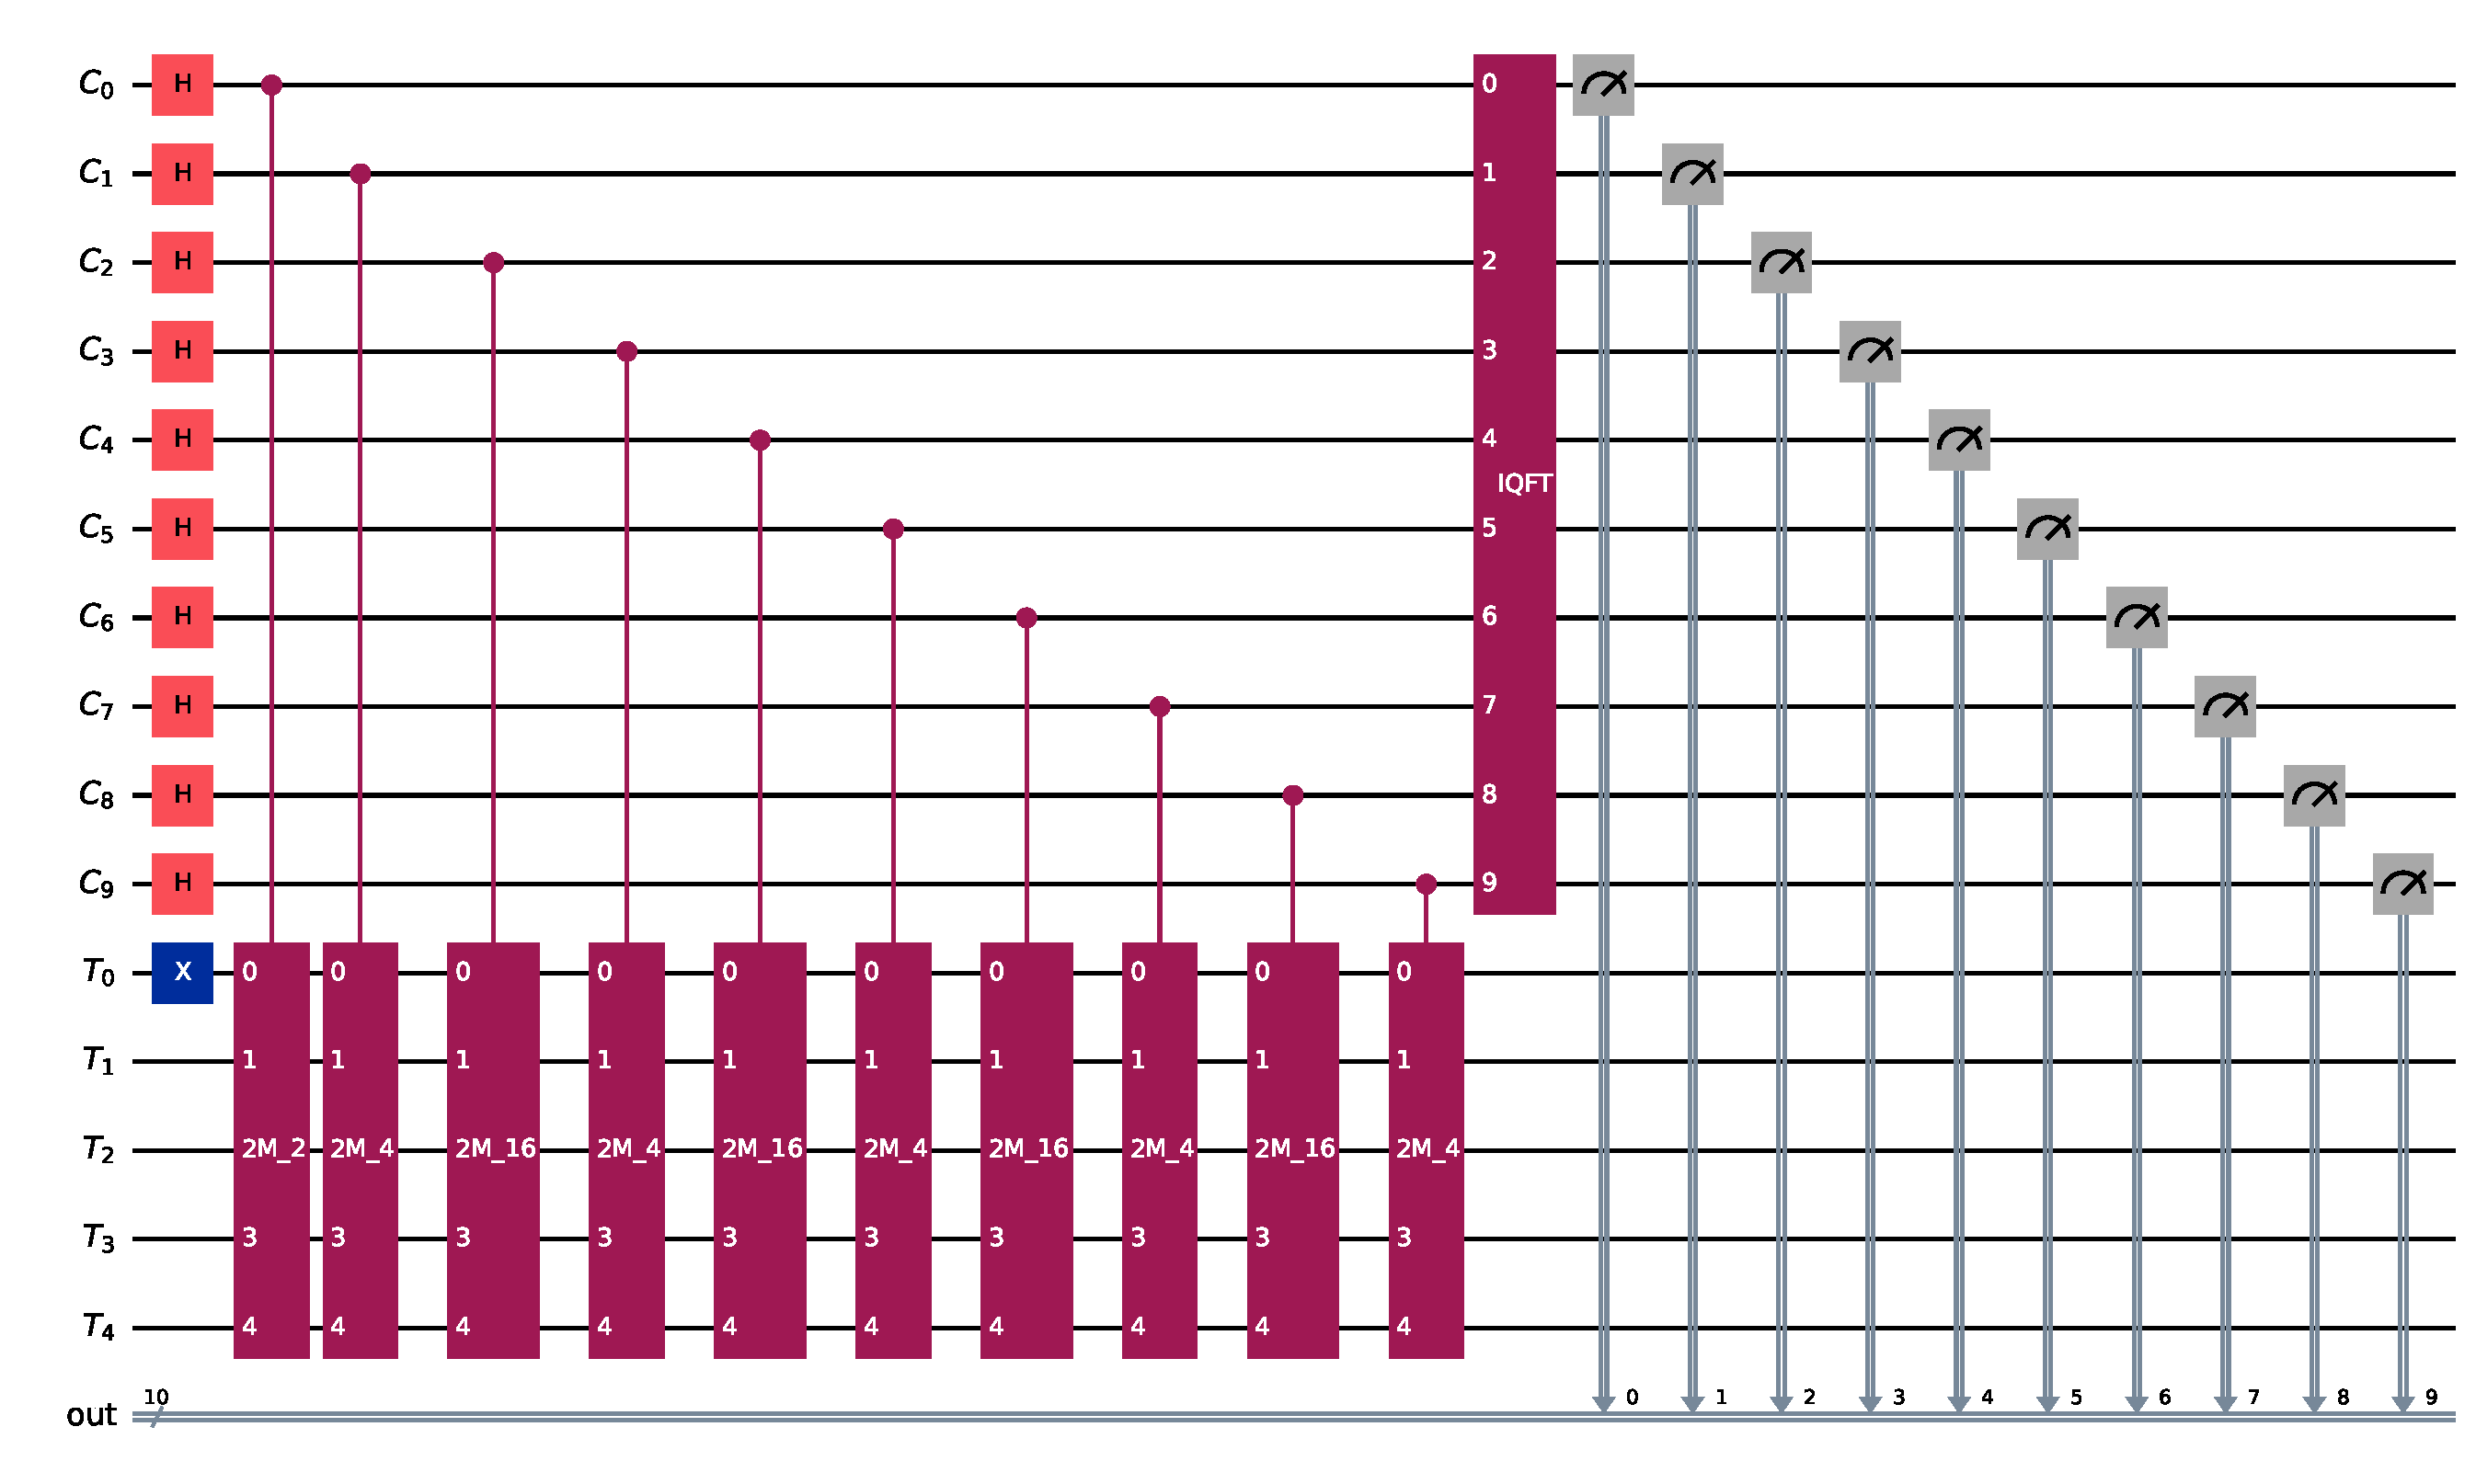
\includegraphics[width=0.65\textwidth]{12_QPE_circuit_N21.pdf}
\caption[Circuito QPE per $N=21$]{Circuito di Quantum Phase Estimation per $N=21$, $a=2$ ($n_{\text{count}}=10$ qubit di controllo, 5 qubit target). La complessità della decomposizione \texttt{UnitaryGate} porta a 10\,040 porte CX dopo la traspilazione.}
\label{fig:qpe_circuit_N21}
\end{figure}

\begin{figure}[H]
\centering
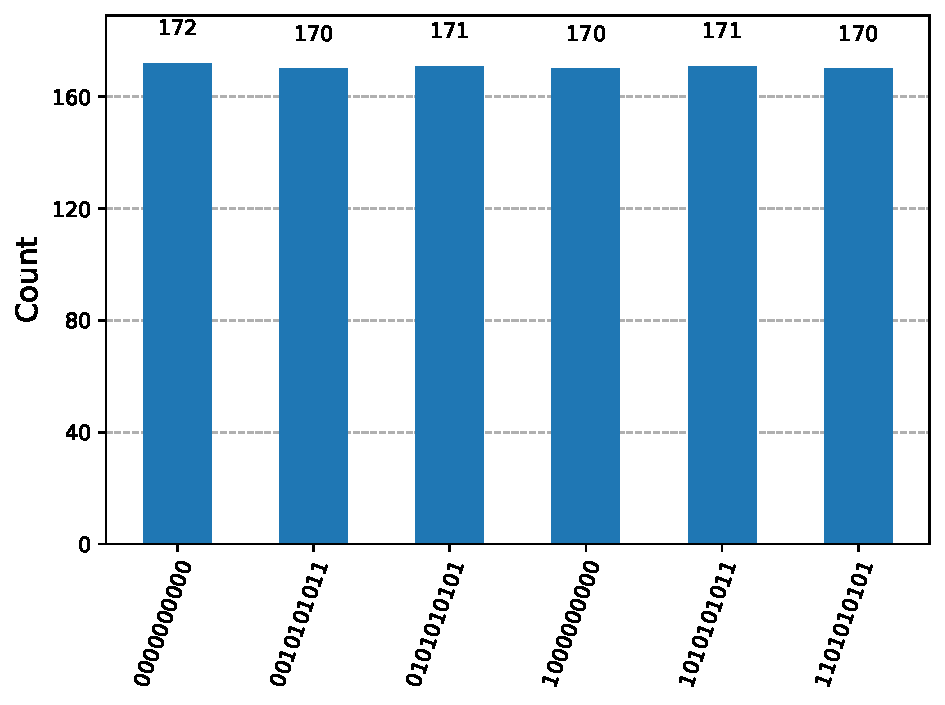
\includegraphics[width=0.7\textwidth]{13_histogram_simulator_N21.pdf}
\caption[Istogramma QPE per $N=21$ — distribuzione piatta]{Distribuzione di misura del registro di controllo per $N=21$ con decomposizione \texttt{UnitaryGate} (1024 shot, noise model NISQ-realistico): l'output è indistinguibile da una distribuzione uniforme.}
\label{fig:histogram_N21_flat}
\end{figure}

% -----------------------------------------------
\section{La Baseline: Metodo 1 (TOP-1)}
\label{sec:risultati_uc_m1}
\label{sec:analisi_m1}
\label{sec:uc1_m1}
\label{sec:uc2_m1}

La Figura~\ref{fig:istogrammi_qpe} mostra i due volti dell'output di UC1: un'iterazione con segnale QPE strutturato (picchi intorno ai valori teorici $\{64, 128, 192\}$) e una in cui il rumore rende l'output quasi uniforme. Distinguere i due casi \emph{prima} della post-elaborazione è esattamente il compito che l'ipotesi iniziale affidava al classificatore.

\begin{figure}[H]
    \centering
    
\includegraphics[width=0.9\textwidth]{fig_istogrammi_qpe.pdf}
    \caption[Confronto istogrammi QPE con segnale strutturato e dominato dal rumore (UC1)]{Confronto tra un istogramma QPE con segnale strutturato (sinistra) e uno dominato dal rumore (destra) per UC1 ($N=15$, NISQ-realistico). I valori teorici attesi per $r=4$ sono $\{64, 128, 192\}$ su $2^8 = 256$ stati.}
    \label{fig:istogrammi_qpe}
\end{figure}

\begin{table}[H]
\centering
\caption{Risultati del Metodo 1 sui quattro use case}
\label{tab:riepilogo_m1}
\begin{tabular}{lcccc}
\hline
\textbf{Use Case} & \textbf{$P_{\text{succ}}$} & \textbf{$\bar{M}_1$} & \textbf{$\sigma_{M_1}$} & \textbf{Mediana} \\
\hline
UC1 ($N=15$, realistico) & 100\% (30/30) & 1.97 & 1.66 & 1.5 \\
UC2 ($N=15$, degradato)  & 100\% (30/30) & 1.60 & 0.76 & 1.0 \\
UC3 ($N=21$)             &  0\%   & N/A  &  ---  & --- \\
UC4 ($N=35$)             &  0\%   & N/A  &  ---  & --- \\
\hline
\end{tabular}
\end{table}

La distribuzione del numero di iterazioni è asimmetrica e approssimativamente geometrica: per UC1 ogni iterazione ha probabilità indipendente $p_{\text{iter}} = 58.3\%$ di produrre la misura corretta tramite TOP-1 (misura diretta su 60 esecuzioni), da cui $\bar{M}_1 \approx 2$. Il dato saliente è che \textbf{la baseline non fallisce mai}: entro il budget di cinquanta iterazioni tutte e trenta le ripetizioni convergono, su entrambi gli use case. La differenza fra i metodi non riguarda dunque \emph{se} il risultato venga trovato, ma \emph{quante esecuzioni} servano per trovarlo --- ed è precisamente ciò che la metrica $\bar{M}$ misura.

Il confronto UC1 vs UC2 rivela un comportamento controintuitivo ($\bar{M}_1$ \emph{minore} sotto rumore maggiore), spiegato dalla banda di accettazione di \texttt{extract\_factors} (\texttt{Fraction.limit\_denominator}): il rumore allarga la distribuzione e aumenta la probabilità che la moda ricada nella banda.

La ragione per cui TOP-1 richiede più di un tentativo è strutturale, e vale la pena isolarla perché anticipa il risultato della sezione seguente. Su sessanta esecuzioni indipendenti di UC1 la moda dell'istogramma cade su uno solo di quattro valori --- $\{0,\,64,\,128,\,192\}$, ossia esattamente i picchi $j\,2^{8}/r$ attesi dalla \ac{QPE} per $r=4$ --- e coincide con l'esito $y=0$ in $25$ casi su $60$ ($41.7\%$), che ne fa l'esito \emph{più frequente in assoluto}. Ma $y=0$ corrisponde a fase nulla e non porta alcuna informazione sul periodo: la funzione di estrazione lo scarta per costruzione. In altri termini, il candidato che TOP-1 seleziona è, in due casi su cinque, quello strutturalmente privo di contenuto informativo; la moda conduce ai fattori nel $58.3\%$ delle esecuzioni, da cui $\bar{M}_1 \approx 1/0.583 = 1.7$, in accordo con il valore misurato $1.97$. Quando invece si considerano i quattro candidati più frequenti, i picchi utili sono presenti in \emph{tutte} e sessanta le esecuzioni: è questa la ragione per cui $M_{\text{TOP4}}$ converge al primo tentativo con deviazione standard nulla.

I limiti della baseline sono dunque due, e motivano il passo successivo: (i) \textbf{spreco informativo} --- TOP-1 usa una sola misura dell'istogramma e scarta tutto il resto, incluso il caso in cui la misura selezionata sia l'esito banale; (ii) \textbf{variabilità} --- $\sigma_{M_1} = 1.66$ contro $\bar{M}_1 = 1.97$: il costo di una sessione resta imprevedibile a priori e non si riduce aumentando gli shot, poiché dipende da quale picco risulti dominante in quella specifica realizzazione del rumore.

% -----------------------------------------------
\section{L'Ipotesi ML alla Prova}

L'ipotesi formalizzata nel Capitolo~\ref{chap:obiettivi} attribuiva la riduzione delle iterazioni a un classificatore \ac{ML}, addestrato a riconoscere gli istogrammi privi di segnale QPE ($\bar{M}_2 \approx 3$, $\rho = \bar{M}_1/\bar{M}_2 > 1$). Sono state addestrate e confrontate tre architetture (Random Forest, \ac{SVM}, \ac{MLP}) su un dataset di 2000 istogrammi per use case: come \emph{classificatori} i modelli funzionano molto bene (F1 fino a 0.98, \ac{AUC} fino a 0.99). L'architettura, la procedura di addestramento e le metriche complete --- con la tabella dei tre modelli e le curve ROC --- sono riportate nell'Appendice~\ref{app:classificatore} (Sez.~\ref{sec:valutazione_clf}). Le metriche di classificazione, però, dicono soltanto che il modello sa distinguere le due classi di istogrammi; la domanda operativa è un'altra --- \emph{questo filtraggio riduce davvero le iterazioni rispetto alla sola ricerca multi-candidato TOP-4?} --- ed è quella a cui risponde l'ablazione seguente.

% -----------------------------------------------
\section{Il Verdetto dell'Ablazione}
\label{sec:confronto}
\label{sec:uc1_m2}
\label{sec:uc2_m2}

\begin{table}[H]
\centering
\caption{Riepilogo comparativo M1, $M_{\text{TOP4}}$ e M2 --- risultato principale con analisi di ablazione ($K=30$, $M_{\text{max}}=50$)}
\label{tab:riepilogo_rho}
\begin{tabular}{llcccc}
\hline
\textbf{UC} & \textbf{Variante} & \textbf{$P_{\text{succ}}$} & \textbf{$\bar{M}$} & \textbf{$\rho$ vs M1} & \textbf{p-value (vs M1)} \\
\hline
\multirow{3}{*}{UC1} & M1 (TOP-1)                 & 100\% & 1.97 & ---            & --- \\
                     & $M_{\text{TOP4}}$ (no clf) & 100\% & 1.00 & \textbf{1.967} & ${<}0.001$ (sign.) \\
                     & M2 (CLF+TOP-4)             & 100\% & 1.03 & 1.903          & ${<}0.001$ (sign.) \\
\hline
\multirow{3}{*}{UC2} & M1 (TOP-1)                 & 100\% & 1.60 & ---            & --- \\
                     & $M_{\text{TOP4}}$ (no clf) & 100\% & 1.00 & \textbf{1.600} & ${<}0.001$ (sign.) \\
                     & M2 (CLF+TOP-4)             & 100\% & 1.57 & 1.021          & $0.315$ (n.s.) \\
\hline
\end{tabular}

\smallskip
{\footnotesize Ablazione $M_{\text{TOP4}}$ vs M2 (Mann-Whitney): UC1 $p = 0.849$ (n.s.); UC2 $p < 0.001$, con M2 che richiede significativamente \emph{più} iterazioni di $M_{\text{TOP4}}$.}
\end{table}

\paragraph{UC1: il classificatore è superfluo.}
M2 raggiunge $\bar{M}_2 = 1{,}03$ con $\rho = 1{,}903$ significativo rispetto a M1: l'ipotesi numerica ($\bar{M}_2 \approx 3$) è addirittura superata. Ma $M_{\text{TOP4}}$ --- TOP-4 \emph{senza} classificatore --- ottiene un risultato migliore ($\bar{M} = 1{,}00$ esatto, con deviazione standard nulla: \emph{ogni} ripetizione converge al primo tentativo), e il confronto $M_{\text{TOP4}}$ vs M2 non è significativo ($p = 0.849$). Il guadagno è interamente della ricerca multi-candidato: il picco QPE si trova sempre tra i quattro candidati più frequenti anche sotto rumore, perché il rumore allarga la distribuzione ma non ne distrugge la struttura --- e, come osservato sopra, il candidato che TOP-1 scarta a favore dell'esito banale $y=0$ viene qui recuperato.

\paragraph{UC2: il classificatore annulla il guadagno.}
M2 produce $\bar{M}_2 = 1{,}57$ contro $\bar{M} = 1{,}00$ del solo $M_{\text{TOP4}}$: il classificatore riporta il costo quasi al livello della baseline ($\rho = 1{,}021$, non significativo rispetto a M1), vanificando il vantaggio che la ricerca multi-candidato aveva ottenuto. Il classificatore \ac{SVM}, addestrato con rumore variato $\pm50\%$, risulta eccessivamente conservativo al rumore nominale di UC2 e scarta iterazioni con segnale QPE parziale che la sola ricerca TOP-4 avrebbe risolto. Rispetto a UC1, dove il filtro è semplicemente inerte, qui esso è attivamente controproducente rispetto alla strategia che accompagna.

\begin{figure}[H]
    \centering
    
\includegraphics[width=0.75\textwidth]{fig_iterazioni_m1_m2.pdf}
    \caption[Analisi di ablazione: M1, $M_{\text{TOP4}}$ e M2 su UC1 ($K=30$)]{Analisi di ablazione su UC1 ($K=30$, $M_{\text{max}}=50$): confronto tra M1 (TOP-1), $M_{\text{TOP4}}$ (TOP-4 senza classificatore) e M2 (CLF+TOP-4). $M_{\text{TOP4}}$ è statisticamente indistinguibile da M2 ($p=0.849$): il guadagno è della strategia TOP-4, non del classificatore.}
    \label{fig:iterazioni_m1_m2}
\end{figure}

\paragraph{Che cosa è stato appurato.}
Il risultato qualitativo dell'ipotesi --- che un approccio multi-candidato riduca $\bar{M}$ --- è confermato per entrambi gli use case tramite $M_{\text{TOP4}}$. La parte dell'ipotesi che attribuiva il guadagno al classificatore è \textbf{smentita}: contributo nullo su UC1, negativo su UC2. Le eccellenti metriche di classificazione non si traducono in guadagno operativo perché \emph{l'informazione che il classificatore estrae dall'istogramma è la stessa che la ricerca TOP-4 sfrutta direttamente}, senza addestramento e senza rischio di falsi negativi. Applicare l'\ac{ML} lì --- a valle dell'esecuzione, sul solo output --- e in quel modo, non ha senso.

% -----------------------------------------------
\section{Robustezza della Strategia TOP-4}
\label{sec:parametri_mitigazione}
\label{subsec:sintesi_parametri}

Identificato il componente attivo, una campagna parametrica sistematica a variazione singola ($K_{\text{rep}}=30$ per punto, test Mann-Whitney) ne ha caratterizzato i margini operativi su sette parametri. Il dettaglio completo, con il confronto previsione/esito per ciascun parametro, è riportato nell'Appendice~\ref{app:parametrica}; la Tabella~\ref{tab:sintesi_parametri} ne riassume gli esiti.

\begin{table}[H]
\centering
\caption{Sintesi della campagna parametrica su $M_{\text{TOP4}}$: impatto atteso, osservato e raccomandazioni}
\label{tab:sintesi_parametri}
\resizebox{\textwidth}{!}{%
\begin{tabular}{lllll}
\hline
\textbf{Parametro} & \textbf{Categoria} & \textbf{Impatto atteso} & \textbf{Impatto osservato} & \textbf{Raccomandazione} \\
\hline
$K$                   & Strategia & Alto ($K = r = 4$)  & Alto ma soglia a $K=2$, non $K=4$              & $K = 2$ minimo; $K = 4$ per margine \\
$\varepsilon_{2q}$    & Rumore    & Alto (dominante)    & Nullo su $M_{\text{TOP4}}$; soglia non trovata  & TOP-K robusto su $[10^{-3}, 10^{-1}]$ \\
$M_{\text{shots}}$    & Strategia & Medio (soglia 1024) & Nullo; 128 shot già sufficienti                & Nessun requisito minimo pratico \\
$T_1$, $T_2$          & Rumore    & Basso (per $N=15$)  & Nullo su $[20\,\mu\text{s}, 500\,\mu\text{s}]$ & Irrilevante per $N=15$ \\
$\varepsilon_{1q}$    & Rumore    & Basso               & Nullo su $[10^{-4}, 2\times10^{-2}]$           & Trascurabile rispetto a $\varepsilon_{2q}$ \\
$p_{\text{ro}}$       & Rumore    & Basso               & Nullo su $[0\%, 20\%]$                         & Irrilevante su tutto il range testato \\
\hline
\end{tabular}%
}
\end{table}

Su sette parametri, uno solo --- $K$ --- ha impatto, con soglia effettiva $K=2$ (più bassa del valore teorico $K=r=4$); tutti gli altri, incluso $\varepsilon_{2q}$ su tre ordini di grandezza, risultano irrilevanti. $M_{\text{TOP4}}$ è quindi applicabile su hardware NISQ senza alcuna calibrazione: il meccanismo non si basa sulla preservazione del segnale QPE \emph{in media} ma sulla sua recuperabilità \emph{per realizzazione} --- come mostra il caso estremo $\varepsilon_{2q}=10^{-1}$, dove la probabilità che nessuna porta a due qubit sbagli è di sei parti su un milione e ciononostante ogni ripetizione converge al primo tentativo.

Il confronto con la \ac{ZNE} sullo stesso task (Tabella~\ref{tab:confronto_zne}; dettaglio in Appendice~\ref{app:parametrica}) completa il quadro. Nessuna delle due varianti di estrapolazione degrada il risultato --- tutte le strategie raggiungono il $100\%$ di successo --- ma nessuna lo migliora in modo significativo: $\bar{M}$ resta statisticamente indistinguibile da quello della baseline, mentre il costo in shot raddoppia o triplica per il campionamento ai livelli di rumore amplificato. La \ac{ZNE} è dunque \emph{inefficace}, non controproducente: paga un prezzo certo per un beneficio che su questo compito non si manifesta. La strategia che accetta il rumore e amplia la ricerca, al contrario, dimezza le iterazioni al costo di un solo campionamento.

\begin{table}[H]
\centering
\caption{Confronto M1, ZNE-2, ZNE-3 e $M_{\text{TOP4}}$ su UC1 ($K_{\text{rep}}=30$, $M_{\text{shots}}=1024$ per livello)}
\label{tab:confronto_zne}
\resizebox{\textwidth}{!}{%
\begin{tabular}{lcccccc}
\hline
\textbf{Strategia} & \textbf{$P_{\text{succ}}$} & \textbf{$\bar{M}$} & \textbf{Shot/iter} & \textbf{Shot totali} & \textbf{$\rho$ vs M1} & \textbf{p-value} \\
\hline
M1 (baseline)             & 100\% & 1.97 & 1024  & 2\,014 & ---   & --- \\
ZNE-2 (lineare)           & 100\% & 2.03 & 2048  & 4\,164 & 0.967 & $0.728$ (n.s.) \\
ZNE-3 (Richardson)        & 100\% & 1.57 & 3072  & 4\,813 & 1.255 & $0.250$ (n.s.) \\
$M_{\text{TOP4}}$ ($K=4$) & 100\% & 1.00 & 1024  & 1\,024 & 1.967 & ${<}0.001$ (sign.) \\
\hline
\end{tabular}%
}
\end{table}

% -----------------------------------------------
\section{Bilancio della Verifica e Ponte verso il Nucleo della Tesi}
\label{sec:top4_mitigazione}
\label{sec:validita}
\label{sec:confronto_zne}

Questa prima fase sperimentale ha appurato tre fatti, tutti con significatività statistica e piena riproducibilità (seed, noise model, circuito e split espliciti e fissati; codice nella repository della tesi):

\begin{enumerate}
    \item la ricerca multi-candidato TOP-4 riduce $\bar{M}$ da 1.97 a 1.00 (UC1), portando ogni ripetizione a convergere al primo tentativo, ed è robusta su tutto il range di rumore NISQ testato, senza addestramento e senza calibrazione;
    \item il classificatore \ac{ML} a valle dell'esecuzione non aggiunge nulla (UC1) o peggiora (UC2): l'ipotesi iniziale, nella parte che attribuiva il guadagno all'apprendimento automatico, era sbagliata --- e l'ablazione lo dimostra;
    \item le tecniche di correzione dell'output (ZNE) sono inefficaci su questo task: non degradano il risultato, ma non lo migliorano in modo significativo e costano da due a tre volte più shot.
\end{enumerate}

Il punto 2 merita di essere letto in positivo, perché delimita con precisione \emph{dove} si ferma ogni strategia a valle: sul solo output, l'informazione utile è già interamente catturata da una ricerca multi-candidato a costo zero --- e ciò che il rumore ha distrutto durante l'esecuzione non è più recuperabile da nessun post-processing, per quanto sofisticato. La conseguenza è strutturale: per andare oltre, l'errore va intercettato e corretto \emph{mentre} il calcolo è in corso, agendo sullo stato quantistico prima che l'informazione sia persa. È esattamente il programma dei prossimi capitoli, che costituiscono il nucleo di questa tesi: la correzione d'errore quantistica --- dal codice a ripetizione al codice di Steane (Capitolo~\ref{chap:qec}), al surface code con la stima sperimentale dell'errore logico (Capitolo~\ref{chap:surface}) --- fino allo Shor logico, che quantifica il livello di correzione necessario all'algoritmo (Capitolo~\ref{chap:integrazione}).

\end{onehalfspace}


% -----------------------------------------------
% Capitolo CORE della tesi: il nuovo approccio (gestione predittiva degli errori)
\chapter{Gestione Predittiva degli Errori: dalla Duplicazione dei Qubit al Machine Learning}
\label{chap:predizione}
\begin{onehalfspace}

Il Capitolo~\ref{chap:risultati} ha chiuso la verifica dell'ipotesi iniziale con un esito netto: applicare l'apprendimento automatico \emph{a valle} dell'esecuzione, sul solo output, non ha senso --- l'informazione contenuta nell'istogramma è già interamente sfruttabile da una ricerca multi-candidato a costo zero. Questo capitolo presenta il nucleo della tesi, che nasce proprio da quel risultato: se l'\ac{ML} deve contribuire alla mitigazione degli errori dell'algoritmo di Shor, deve operare \emph{a monte}, sull'informazione che nell'output non c'è --- la fisica del dispositivo. Nelle sezioni che seguono si descrive il problema (gli errori hardware non sono uniformi, ma sistematici e quindi prevedibili), la soluzione oggi adottata dall'industria (la duplicazione dei qubit), la proposta di questa tesi (un modello predittivo degli errori addestrato sulla specifica \mbox{QPU}) e l'architettura del sistema con cui intendiamo realizzarla e validarla.

% -----------------------------------------------
\section{Il Problema: gli Errori Hardware non sono Uniformi}
\label{sec:errori_non_uniformi}

Il Capitolo~\ref{chap:rumore} ha analizzato le quattro fonti fisiche di errore dei processori \ac{NISQ}: la decoerenza ($T_1$, $T_2$), gli errori di gate, gli errori di misura (\textit{readout}) e il crosstalk. Nella modellazione adottata finora --- come nella maggior parte della letteratura introduttiva --- questi errori sono stati trattati come proprietà \emph{globali} del dispositivo: un unico $T_1$, un unico tasso $\varepsilon_{2q}$, un'unica probabilità di errore di lettura per tutti i qubit. La realtà fisica di una \ac{QPU} è diversa, e questa differenza è il punto di partenza dell'intero approccio proposto.

\paragraph{La decoerenza varia da qubit a qubit.}
I qubit superconduttori sono strutture litografiche a scala molecolare: imperfezioni nel processo di fabbricazione (ad esempio nell'ossidazione delle giunzioni Josephson) fanno sì che, sullo stesso chip, un qubit possa esibire $T_1 = 100\,\mu\text{s}$ e il suo vicino $T_1 = 30\,\mu\text{s}$. La conseguenza operativa è severa: quando due qubit vengono posti in entanglement, la coerenza della coppia decade con il \emph{peggiore} dei due --- il qubit da $100\,\mu\text{s}$ viene trascinato a $30\,\mu\text{s}$, e quando uno dei due decade, l'informazione condivisa è persa per entrambi. Un algoritmo che ignora questa disomogeneità è costretto a dimensionarsi sul qubit più debole della linea utilizzata; il rischio cresce quando il tempo di esecuzione del circuito si avvicina al bordo della finestra di coerenza, dove la probabilità di decadimento è massima.

\paragraph{I gate sono hardware, e ogni linea è diversa.}
Le porte logiche quantistiche non risiedono nel chip: sono impulsi a microonde generati dall'elettronica di controllo esterna e convogliati ai qubit tramite guide d'onda. Lo stesso gate logico, applicato a linee diverse, può richiedere tempi diversi ed esibire fedeltà diverse; un impulso impreciso ruota lo spin di un angolo sbagliato, producendo uno stato errato che si manifesta solo alla misura. Il tempo di gate --- decine di nanosecondi sui superconduttori, millisecondi sugli ioni intrappolati --- è il secondo parametro fondamentale insieme alla coerenza: il numero massimo di operazioni eseguibili è il rapporto tra la finestra di coerenza e la durata del singolo gate, ed è questo rapporto (non il solo $T_1$) a determinare se una \ac{QPU} può fisicamente sostenere il circuito di Shor per una data istanza.

\paragraph{La misura è essa stessa una sorgente di errore.}
La lettura di un qubit avviene bombardandolo con una microonda e osservando la risposta: è un processo fisico che distrugge lo stato e che, se il qubit è prossimo alla fine della coerenza, può restituire 0 per 1 o viceversa. Questi errori si caratterizzano tramite matrici di confusione ottenute preparando stati noti e misurandone le distribuzioni di lettura. Nei dispositivi commerciali l'affidabilità di lettura considerata accettabile parte dal 95\%: un errore intrinseco superiore al 5\% rende il dato inutilizzabile.

\paragraph{Il crosstalk dipende dalla topologia.}
I qubit adiacenti sul chip si accoppiano capacitivamente: operare su un qubit perturba i vicini con rotazioni parassite non intenzionali, e la stessa microonda di controllo o di lettura, per quanto focalizzata, raggiunge parzialmente i qubit circostanti. L'entità del fenomeno dipende dalla \emph{geometria} del dispositivo --- una catena lineare, una griglia, una connettività completa --- e dalle linee di accoppiamento fisico effettivamente presenti: su una topologia a catena, l'entanglement tra qubit non adiacenti richiede operazioni intermedie che amplificano il disturbo e accorciano la vita dello stato condiviso.

\paragraph{Sistematicità, quindi prevedibilità.}
Il punto cruciale è che questi difetti non sono rumore bianco: sono \textbf{caratteristiche stabili del singolo esemplare fisico}. Se una linea di qubit fallisce otto volte su dieci per circuiti di una certa profondità, quella linea è \emph{sistematicamente} debole per quella classe di input --- e continuerà a esserlo. La profondità del circuito di Shor dipende dall'istanza ($N$ piccolo usa meno gate di $N$ grande), per cui una stessa linea può essere adeguata per certi input e inadeguata per altri. Un comportamento sistematico e dipendente da variabili osservabili (quale linea, quale input, quale profondità) è, per definizione, un comportamento \emph{apprendibile}.

% -----------------------------------------------
\section{La Pratica Attuale: la Duplicazione dei Qubit}
\label{sec:duplicazione}

Come gestisce oggi l'industria l'inaffidabilità dei singoli qubit? Il teorema di no-cloning (Capitolo~\ref{chap:fondamenti}) impedisce la soluzione classica più ovvia: non è possibile copiare uno stato quantistico durante l'esecuzione, né "trasferire" il calcolo da un qubit morente a uno sano. La tecnica adottata è la \textbf{duplicazione}: per ogni qubit logico dell'algoritmo se ne impiegano due fisici, e l'intero calcolo viene raddoppiato.

Operativamente, si eseguono \emph{due istanze gemelle} dell'algoritmo di Shor in parallelo, sugli stessi dati, su due linee di qubit diverse del dispositivo: i registri iniziali vengono preparati in modo identico ($A_1$/$A_2$, $B_1$/$B_2$, \ldots), le due istanze evolvono indipendentemente, e alla fine si leggono gli stati di entrambe. È più probabile che, su due copie, almeno una arrivi viva alla misura: dove una copia risulta decaduta o illeggibile, si utilizza l'informazione dell'altra. Poiché le due istanze operano sugli stessi input, non possono produrre soluzioni valide diverse: se entrambe sopravvivono concordano, se una muore si usa la superstite, se muoiono entrambe l'esecuzione è da ripetere.

Il costo di questa strategia è diretto e severo: \textbf{il fabbisogno di qubit fisici raddoppia}. Per l'istanza crittograficamente rilevante --- fattorizzare un modulo RSA a 2048 bit, che richiede $\sim$2048 qubit logici --- servono $\sim$4096 qubit fisici. L'esperienza pratica mostra inoltre rendimenti decrescenti: raddoppiare conviene, triplicare o quadruplicare no --- il guadagno di affidabilità aggiuntivo non giustifica il costo, proprio perché il meccanismo agisce solo sulla probabilità di sopravvivenza e non sulla \emph{causa} dei fallimenti.

La duplicazione ha infine tre limiti strutturali che la rendono un bersaglio naturale per un approccio più intelligente:
\begin{itemize}
    \item è \textbf{agnostica rispetto al dispositivo}: tratta tutti i qubit come ugualmente inaffidabili, ignorando che i difetti sono localizzati e stabili;
    \item \textbf{spreca conoscenza}: ogni esecuzione rivela quali linee hanno fallito, ma questa informazione non viene accumulata né riutilizzata;
    \item \textbf{consuma metà della QPU}: la capacità computazionale effettiva del dispositivo è dimezzata in modo permanente, indipendentemente da quanto la specifica esecuzione ne avrebbe avuto bisogno.
\end{itemize}

% -----------------------------------------------
\section{La Proposta: un Modello Predittivo degli Errori}
\label{sec:proposta_predittiva}

La proposta di questa tesi è sostituire la ridondanza fisica con la \textbf{conoscenza appresa del dispositivo}: un modello di apprendimento automatico, addestrato sul comportamento della specifica \ac{QPU}, che predica dove e quando gli errori si manifesteranno.

\paragraph{Perché qui l'ML ha senso (e a valle no).}
La verifica del Capitolo~\ref{chap:risultati} ha dimostrato che un classificatore che osserva il solo istogramma di output non aggiunge nulla: quell'informazione è già catturata dalla ricerca TOP-K. Il modello proposto attinge invece a informazione \emph{strutturale}, che nessuna strategia a valle può vedere: la topologia del dispositivo, i tempi di coerenza dei singoli qubit, quali linee il circuito attraversa, la profondità richiesta dall'input. È la differenza tra giudicare una fotografia sfocata e conoscere quale lente dell'obiettivo è graffiata: la seconda conoscenza permette di \emph{prevedere} la sfocatura prima dello scatto, e di scegliere una lente diversa.

\paragraph{Che cosa promette il modello.}
Il livello minimo di funzionalità --- sufficiente a giustificare l'approccio --- è la \textbf{segnalazione}: dato l'esito di un'esecuzione e le condizioni in cui è avvenuta, il modello indica "questo risultato è probabilmente errato". Non serve conoscere la risposta giusta: la sola segnalazione affidabile permette di scartare l'esito e reiterare, esattamente come la strategia TOP-K permetteva di evitare iterazioni sprecate. Il livello avanzato è la \textbf{prescrizione}: per un dato tipo di input, il modello indica quali linee di qubit evitare ("per questa profondità di circuito, la linea 1 fallisce sistematicamente: usa la seconda"), instradando l'esecuzione sulle risorse fisiche più adatte \emph{prima} di consumarle.

\paragraph{Un modello per esemplare, non per modello.}
Poiché i difetti sono caratteristiche del singolo chip --- due esemplari identici dello stesso modello di QPU hanno mappe di difetti diverse --- il modello va addestrato \emph{su quella specifica QPU}, con una fase di caratterizzazione basata su input a verità nota. Questo è un costo una-tantum per dispositivo, analogo alla calibrazione periodica che i provider già eseguono, ma il suo prodotto è riutilizzabile per ogni esecuzione successiva.

\paragraph{Il claim da validare.}
La promessa quantitativa, che la fase sperimentale dovrà verificare, si formula così: \emph{l'algoritmo di Shor eseguito in copia singola, assistito dal modello predittivo, raggiunge un'affidabilità almeno pari a quella della duplicazione, utilizzando la metà dei qubit fisici}. Se il claim regge, il messaggio pratico è quello indicato dal relatore: chi implementa Shor non ha più bisogno di duplicare --- esegue una copia sola e lascia che il modello, addestrato su quella macchina, faccia il resto.

% -----------------------------------------------
\section{Architettura del Sistema Proposto}
\label{sec:architettura_predittiva}

Il sistema si compone di quattro elementi, progettati per essere realizzati con l'infrastruttura sperimentale già sviluppata (Capitoli~\ref{chap:strumenti} e~\ref{chap:sviluppo}) opportunamente estesa.

\paragraph{1. QPU virtuale con iniezione di errori configurabile.}
Il primo componente è un simulatore di \ac{QPU} in cui le quattro categorie di errore sono configurabili \emph{per singolo qubit e per singola linea}, non globalmente: a ogni qubit i propri $T_1$/$T_2$, a ogni coppia accoppiata la propria fedeltà e durata di gate, a ogni linea di lettura il proprio errore di misura, e un modello di crosstalk derivato dalla topologia dichiarata (quali qubit sono fisicamente accoppiati con quali). Rispetto al noise model uniforme utilizzato nella fase di verifica, questa è un'estensione sostanziale ma tecnicamente percorribile: Qiskit Aer supporta nativamente errori per-qubit e coupling map, mentre il crosstalk andrà modellato come canale di errore correlato sui vicini topologici. La QPU virtuale si comporta come una QPU reale --- "su dieci gate che passano, a volte uno sbaglia" --- ma con percentuali e localizzazione dei difetti decise da noi, e quindi note.

\paragraph{2. Dataset a verità nota.}
Il secondo componente è la campagna di caratterizzazione: si costruisce un insieme di istanze di fattorizzazione con soluzione nota (semiprimi $N = p \times q$ con $p$, $q$ primi scelti, di profondità circuitale crescente) e lo si esegue ripetutamente sulla QPU virtuale --- nell'ordine del migliaio di esecuzioni per configurazione. Poiché input, output atteso e profilo di errore iniettato sono tutti noti, ogni esecuzione produce un esempio etichettato: quali linee erano coinvolte, quale profilo di errore era attivo, e se l'esito era corretto.

\paragraph{3. Modello predittivo con feature strutturali.}
Il terzo componente è il modello di apprendimento: le feature comprendono la descrizione della QPU (topologia, $T_1$/$T_2$ per qubit, fedeltà di gate per linea), la descrizione dell'esecuzione (linee utilizzate, profondità del circuito, tipo di input) e l'esito osservato; le etichette derivano dalla verità nota. L'architettura del modello (classificatore, regressore di affidabilità per linea, o sistema a due stadi) è una scelta progettuale aperta, da guidare con lo stesso rigore comparativo usato nella fase di verifica. Un'estensione avanzata segnalata dal relatore --- l'uso delle matrici di confusione come spazio hamiltoniano in ingresso a un algoritmo \ac{QAOA} per identificare gli errori trascurabili --- è deliberatamente esclusa dal perimetro di questa fase per la sua complessità, e rimandata agli sviluppi futuri.

\paragraph{4. Protocollo di validazione con baseline di duplicazione.}
Il quarto componente incorpora la lezione metodologica della fase di verifica: \emph{l'ablazione si progetta dall'inizio, non si aggiunge dopo}. Il confronto sperimentale prevede tre bracci fin dal disegno: (a) copia singola senza modello (baseline inferiore), (b) \textbf{duplicazione dei qubit} --- da implementare come baseline di riferimento, poiché è la pratica che il modello intende sostituire --- e (c) copia singola assistita dal modello predittivo. Le metriche sono il tasso di successo, il numero di iterazioni e il costo in qubit fisici; la significatività statistica sarà valutata con gli stessi strumenti non parametrici già adottati (Mann-Whitney, $K \geq 30$ ripetizioni).

% -----------------------------------------------
\section{Ipotesi Operative e Criteri di Successo}
\label{sec:ipotesi_predittiva}

La fase sperimentale è guidata da due ipotesi verificabili:

\begin{enumerate}
    \item \textbf{Ipotesi di prevedibilità}: sugli errori generati dalla QPU virtuale con difetti localizzati e stabili, un modello addestrato con feature strutturali raggiunge una capacità di segnalazione degli esiti errati significativamente superiore al caso ($\text{AUC} > 0.5$ con margine statisticamente significativo), e crescente con la sistematicità dei difetti iniettati.
    \item \textbf{Ipotesi di sostituzione}: la copia singola assistita dal modello eguaglia o supera il tasso di successo della duplicazione a parità di iterazioni, con la metà dei qubit fisici. Criterio quantitativo: differenza di tasso di successo non inferiore (test unilaterale, $p < 0.05$) rispetto al braccio duplicato.
\end{enumerate}

Diversamente dalla fase di verifica --- dove le metriche di classificazione eccellenti nascondevano l'assenza di guadagno operativo --- il criterio di successo primario è qui direttamente operativo (ipotesi 2), e le metriche di apprendimento (ipotesi 1) hanno il solo ruolo di diagnostica intermedia. La realizzazione sperimentale di questo programma --- l'implementazione della QPU virtuale, la generazione del dataset, l'addestramento e la validazione comparativa --- costituisce la prossima fase del lavoro; le estensioni oltre questo perimetro, dalla validazione su hardware fisico reale all'integrazione con la correzione d'errore strutturale, sono discusse nel Capitolo~\ref{chap:sviluppi}.

\end{onehalfspace}


% -----------------------------------------------
\chapter{Sviluppi Futuri}
\label{chap:sviluppi}
\begin{onehalfspace}

I risultati delimitano con chiarezza ciò che la demo e la campagna
dimostrano: l'esecuzione ideale è verificata anche per $N=21/35$, mentre
il confronto controllato fra canali di rumore è sostenibile su $N=15$.
Le estensioni seguenti mirano a colmare questa distanza senza
estrapolare i risultati oltre il loro perimetro.

% -----------------------------------------------
\section{Scalabilità a Istanze di Maggiore Dimensione}
\label{sec:scalabilita_futura}

La priorità è ridurre il costo dell'aritmetica modulare. La costruzione
Beauregard implementata nella tesi è stata validata idealmente mediante
truth table e distribuzione QPE, ma per $N=21$, $a=2$ e otto controlli il
circuito esecutivo compilato nella base \texttt{rz/sx/x/cx} contiene
21\,036 CX e ha profondità 23\,081. Questi sono conteggi della
compilazione congiunta, non somme di blocchi né stime su un gate set più
astratto.

Le direzioni immediate sono l'approximate QFT con soglia d'angolo
esplicita, addizionatori alternativi, sintesi mirata al gate set del
backend e riduzione delle operazioni controllate prima della
traspilazione. Ogni variante dovrebbe superare gli stessi controlli già
usati qui: verità funzionale della moltiplicazione, ancille pulite,
coerenza di fase e distanza della QPE ideale dalla legge teorica. Il
numero di gate, da solo, non è una prova di correttezza.

Anche la scelta delle istanze deve essere governata dall'ordine
moltiplicativo $r$, non soltanto dal modulo $N$. L'istanza $N=35$, $a=6$
ha ordine 2 e non costituisce una progressione monotona rispetto a
$N=21$, $a=2$, che ha ordine 6. Una campagna di scalabilità dovrebbe
quindi stratificare sia la larghezza sia l'ordine e dichiarare a priori
quale delle due variabili intende studiare.

% -----------------------------------------------
\section{Ottimizzazione della Trasformata di Fourier Consapevole della Topologia}
\label{sec:qft_topologia}

La direzione precedente indica l'approximate QFT fra le varianti da esplorare.
Una campagna esplorativa condotta a chiusura del lavoro ne ha misurato il margine, e il
risultato merita di essere riportato perché delimita l'intera famiglia di ottimizzazioni
di questo tipo.

\paragraph{Controllo su $N=15$ ed eliminazione degli SWAP.}
Nel pilota su $N=15$, la configurazione $k_{\mathrm{QPE}}=1$, scelta sui
batch di selezione, ottiene sull'holdout $0.6279$ contro $0.4792$ della
QFT piena: differenza $+0.1487$, IC Newcombe 95\%
$[+0.1273;+0.1699]$, con 279 ECR invece di 362. Il beneficio riguarda
un caso favorevole e degenere, con fasi esatte in due bit, e non dimostra
lo stesso effetto per ordini più lunghi. L'eliminazione degli SWAP di
inversione dei bit produce invece conteggi compilati e risultati
identici: il transpiler ne assorbe già la permutazione nel layout.
Griglia, controllo della variante corretta e risultati completi sono
nella Sezione~\ref{sec:app_aqft} dell'Appendice~\ref{app:fase2}.

Nell'aritmetica di Beauregard, gran parte del costo viene dalle QFT interne agli addizionatori modulari. Per $N=21$ si contano 11\,436 porte \texttt{cp} e 3\,406 \texttt{cx}; la QFT finale richiede invece solo 28 rotazioni, su circa 47\,000 porte complessive. Eliminare le rotazioni più piccole negli addizionatori porta le porte a due qubit da 49\,661 a 23\,178. Agire sulla sola trasformata finale non cambia l'ordine di grandezza. Il primo controllo identifica quindi la parte del circuito su cui conviene intervenire.

Ridurre le porte comporta una perdita di precisione. Su $N=21$, il successo ideale scende da $0{,}4667$ a $0{,}4013$, cioè di circa sei punti e mezzo. In presenza di rumore, la variante troncata può recuperare questa perdita solo se il risparmio di porte evita abbastanza errori. Il bilancio dipende quindi dalla qualità delle porte e va verificato.

Un modello semplificato combina il successo ideale con quello di una distribuzione uniforme. In questo modello, il vantaggio massimo stimato della variante troncata è circa \textbf{tre punti percentuali}. Richiederebbe errori a due qubit circa \textbf{duecento volte inferiori} a quelli dei dati di calibrazione considerati. È una stima del modello, non un vantaggio misurato né un limite universale. Nei test rumorosi non emerge un beneficio statisticamente significativo del troncamento. Al rumore nominale, le configurazioni provate restano vicine al livello uniforme; nel punto in cui compare un segnale, è la QFT \emph{piena} ad avere il risultato migliore. Il circuito di $N=21$ dura circa centocinquanta volte il tempo di coerenza tipico. Questa profondità limita la possibilità di distinguere le varianti nel regime considerato.

Per capire se il limite dipenda dal costo di Shor, si ripete il confronto sulla sola \textbf{stima di fase}. Con un unitario di fase, il circuito richiede decine di porte a due qubit, anziché decine di migliaia. I nove confronti usano tre dimensioni di registro e fasi sia esattamente rappresentabili sia non rappresentabili in $n$ bit. La variante troncata ha un risultato migliore in \textbf{tutti e nove}; in sei, l'intervallo di confidenza è interamente positivo. Su dieci qubit il vantaggio raggiunge $+0{,}126$, con IC Newcombe 95\% $[+0{,}098;\ +0{,}153]$.

Nei test sulla stima di fase emergono tre regolarità. Il grado migliore di troncamento resta \textbf{due o tre} alle taglie provate, mentre la QFT piena usa $n-1$. Il risparmio cresce così da venticinque porte a due qubit su sei qubit a settantotto su dieci. Cresce anche il vantaggio, da circa due a tredici punti percentuali. Infine, le fasi esattamente rappresentabili beneficiano più delle altre. Questo aiuta a interpretare la differenza fra le istanze di Shor: per $N=15$, l'ordine $r=4$ dà fasi $0$, $1/4$, $1/2$, $3/4$, esatte in due bit. Per $N=21$, l'ordine $r=6$ dà invece fasi $j/6$, per le quali le rotazioni fini conservano informazione utile.

La prima di queste regolarità --- quella che a prima vista sorprende di più, perché un
registro più lungo sembrerebbe richiedere più rotazioni fini --- ha una spiegazione
teorica indipendente, pubblicata mentre questo lavoro era in corso. Akoramurthy e
Surendiran derivano per la stima di fase con trasformata troncata un limite in forma
chiusa sulla distanza in variazione totale fra la distribuzione esatta e quella
troncata~\cite{akoramurthy2026}:
%
\begin{equation}
\mathrm{TV}\!\left(P_\phi,\, P_\phi^{d}\right) \;\le\; \frac{\pi\,(m-d)}{2^{d}},
\label{eq:bound_troncamento}
\end{equation}
%
dove $m$ è la dimensione del registro e $d$ il grado di troncamento. Il numeratore cresce
linearmente in $m$, il denominatore esponenzialmente in $d$: per mantenere
fisso il limite al crescere del registro occorre far crescere $d$ circa
logaritmicamente. Il grado piccolo osservato alle tre taglie provate
non dimostra dunque che un grado costante basti a qualunque dimensione. Gli autori
riportano inoltre una riduzione del $31{,}3$--$43{,}7\%$ nel conteggio di porte e un
passaggio di complessità da $O(m^2)$ a $O(m \log m)$ per $d = O(\log m)$. Il loro impianto
sperimentale si ferma però alla stima di fase e non affronta la fattorizzazione: la
delimitazione riportata sopra --- che su Shor la stessa leva vale al massimo tre punti
percentuali, e solo con porte a due qubit molto più accurate delle attuali --- resta
propria di questo lavoro, così come la selezione del grado su dati disgiunti da quelli di
verifica.

Conteggi di porte e calibrazione permettono di proporre gradi candidati
prima dell'esecuzione. In questa campagna, però, il grado viene scelto
empiricamente sui batch di selezione e verificato su holdout disgiunti:
non è stata validata una scelta ottima dai soli conteggi. Il contributo
è quindi un criterio di progetto e un protocollo di verifica per la
trasformata, da controllare quando cambia l'algoritmo o il dispositivo.

Un'estensione consiste nel combinare tre riduzioni. La prima, misurata qui, approssima la QFT per usare meno \emph{porte}. La seconda approssima l'aritmetica modulare per usare meno \emph{qubit di lavoro}~\cite{chevignard2025} e contribuisce alle recenti stime di risorse~\cite{gidney2025}. La Tabella~\ref{tab:traiettoria_risorse} ne riporta l'evoluzione e le assunzioni. La terza divide la stima di fase in blocchi indipendenti per ridurre i \emph{qubit di conteggio}~\cite{shukla2026}.

I tre risparmi non si sommano automaticamente. Ridurre i qubit di lavoro può richiedere più porte: per RSA-2048, una proposta passa da 6144 a 1730 qubit logici, ma porta i Toffoli da $2^{31{,}3}$ a $2^{40{,}9}$~\cite{chevignard2025}. Ottimizzazioni aritmetiche successive recuperano parte di questo costo~\cite{gidney2025}. Combinare la riduzione dei qubit con il troncamento della QFT richiede quindi di misurare il bilancio finale delle porte.

La riduzione del registro di conteggio agisce invece sulla stima di fase e lascia invariato il registro di lavoro~\cite{shukla2026}. La proposta passa da $2n+1$ a tre o quattro qubit di conteggio. Blocchi indipendenti stimano più bit di fase, poi un procedimento dal bit meno significativo al più significativo risolve le ambiguità~\cite{shuklaqpe2026}. Per verificare se questa riduzione sia compatibile con le altre, occorre un esperimento che le combini e misuri anche la profondità. Le singole proposte sono quantificate; il loro beneficio congiunto resta da dimostrare.

La QFT compare anche nella stima di fase, nell'amplitude estimation, nel conteggio quantistico, nella risoluzione di sistemi lineari e nel problema del sottogruppo nascosto, di cui Shor è un caso particolare. Si usa inoltre nelle simulazioni che alternano rappresentazioni in posizione e in momento. Questi algoritmi impiegano le stesse rotazioni controllate di piccolo angolo. Il protocollo seguito qui può suggerire verifiche analoghe: proporre gradi di troncamento dai conteggi, sceglierli su dati di selezione e valutarli su dati indipendenti. Queste verifiche restano da eseguire. Il contributo è quindi un metodo di valutazione, con risultati limitati ai circuiti provati.

Il pilota incompleto su $N=21$, i tre livelli di sensibilità al rumore,
la distinzione fra configurazione scelta e variante troncata, e i nove
contrasti QPE sono documentati nelle Tabelle~\ref{tab:aqft_n21_sensibilita}
e~\ref{tab:aqft_qpe_completa}. Sono riportati anche gli esiti negativi
e i contrasti i cui intervalli includono lo zero.

La verifica usa un layout per dimensione, una sola calibrazione e tre fasi bersaglio. Le varianti condividono batch e semi, quindi il confronto interno usa gli stessi campioni. Il risultato non dimostra però che il beneficio si mantenga su altri dispositivi o topologie.

Il precedente più vicino è la compilazione \emph{noise-adaptive}, che ordina o vincola il
collocamento del circuito usando i dati di calibrazione~\cite{murali2019, tannu2019}. La
differenza rispetto a quella linea, e il motivo per cui resta spazio, è che tali metodi
ottimizzano la fedeltà del circuito, mentre per un algoritmo come Shor conta soltanto che
il post-processing restituisca i fattori. I due obiettivi non coincidono, e la campagna
sulla compilazione riportata in Appendice~\ref{app:fase2} misura quanto non coincidano.

% -----------------------------------------------
\section{Validazione su Hardware Quantistico Reale}
\label{sec:hw_reale}

Va anzitutto dichiarato che l'assenza di esecuzione su hardware è una
\textbf{scelta deliberata e concordata}, non una questione rimasta
irrisolta: pur essendo divenuto disponibile in corso d'opera l'accesso a
un dispositivo, si è convenuto di non impiegarlo, poiché le domande
sperimentali del lavoro erano già state chiuse sui modelli di rumore e
sulle snapshot di calibrazione. L'intera validazione riportata in questa
tesi appartiene quindi a quel perimetro, e ogni confronto con una
macchina reale resta un lavoro successivo, di cui questa sezione descrive
il protocollo.

Il modello rumoroso della tesi è uniforme e illustrativo: non include
coupling map, routing, crosstalk, leakage o deriva della calibrazione. Il
passo successivo è ripetere il protocollo $N=15$ su una QPU, registrando
backend, timestamp, proprietà dei qubit, layout iniziale e finale,
conteggi post-routing e job identifier. Il confronto deve usare lo stesso
budget di shot e una politica di seed dichiarata, senza presentare il
preset uniforme come replica della macchina.

La demo è già predisposta per questo confronto metodologico: distingue
rumore disattivato, scenario moderato, scenario di stress e canali
singoli. Un'estensione hardware dovrebbe affiancare una quinta modalità
``calibrazione acquisita'', costruita dallo snapshot reale e marcata con
la sua data di validità. In questo modo diventerebbe misurabile il
\emph{simulation gap} fra il modello controllato e il dispositivo.

Per $N=21/35$ l'hardware non elimina il problema della profondità: evita
il costo esponenziale dello statevector classico, ma non le migliaia di
operazioni rumorose e i vincoli di connettività. Prima di eseguire queste
istanze servono quindi una sintesi più corta e un budget d'errore basato
sul circuito effettivamente instradato.

% -----------------------------------------------
\section{Generalizzazione ad Altri Algoritmi Quantistici}
\label{sec:altri_algoritmi}

TOP-K è utile soltanto quando più candidati possono essere verificati
classicamente a costo contenuto. Questa proprietà vale per Shor, perché
ogni candidato al periodo produce o meno divisori verificabili, e può
valere per problemi di ricerca con un oracolo di verifica. Non segue
automaticamente che la stessa strategia migliori VQE~\cite{peruzzo2014} o
QAOA~\cite{farhi2014}, dove
l'output centrale è una stima di valore atteso e non una lista di
soluzioni equivalenti.

Una generalizzazione corretta dovrebbe quindi definire prima:
\begin{enumerate}
    \item una funzione classica di validazione del candidato;
    \item il costo aggiuntivo delle $K$ verifiche;
    \item una baseline TOP-1 appaiata sugli stessi campioni;
    \item un criterio che impedisca a $K$ di rendere il successo quasi
    certo per puro effetto combinatorio.
\end{enumerate}
Grover su problemi con verifica economica è un primo banco di prova;
per gli algoritmi variazionali è invece più naturale studiare
allocazione adattiva degli shot o mitigazione del bias dell'osservabile.

% -----------------------------------------------
\section{Integrazione con la Quantum Error Correction}
\label{sec:qec_integrazione}

La campagna di Shor logico usa $p_L$ come probabilità fenomenologica di
Pauli non-identità per gate compilato incluso nel proxy. Non identifica questo parametro con
il logical error rate di un memory experiment surface-code: le due
grandezze hanno circuiti, osservabili e granularità differenti. Il passo
successivo scientificamente significativo è una mappatura esplicita fra
un set di operazioni logiche fault-tolerant e i canali residui stimati per
ciascuna operazione.

Solo dopo tale mappatura sarebbe lecito combinare surface code e Shor in
una previsione end-to-end. Servirebbero almeno: conteggio delle operazioni
logiche per tipo, costo di magic-state distillation per le non-Clifford,
decoder e latenza di feed-forward, errori correlati e intervalli di
confidenza propagati. Il modello fenomenologico della tesi resta utile
come analisi di sensibilità, non come stima di risorse hardware.

Per la decodifica appresa, le direzioni più promettenti restano modelli a
grafo o convoluzionali che rispettino la località del reticolo, uso della
storia temporale dei cicli e soft information analogica della misura.
Queste estensioni aggiungono informazione o struttura; non si limitano a
ingrandire una rete densa sullo stesso vettore di sindrome.

% -----------------------------------------------
\section{Evoluzione del Classificatore ML}
\label{sec:evoluzione_ml}

La campagna aggiornata mostra che TOP-1 è addestrabile ma operativo solo
come predittore della riuscita del candidato dominante; TOP-16 produce
invece $2\,000/2\,000$ positivi in entrambi gli scenari. Inoltre M2 è
peggiore della propria ablazione TOP-4 nei due confronti appaiati. Non è
quindi giustificato migliorare soltanto l'architettura mantenendo la
stessa etichetta.

Un nuovo problema supervisionato dovrebbe prevedere un obiettivo legato
al costo, ad esempio il valore atteso degli shot risparmiati dopo aver
considerato il costo di uno scarto errato. Training e test dovrebbero
essere separati anche per giorno di calibrazione o backend, non solo per
seed, e la soglia decisionale scelta su validation. Prima di addestrare
si deve infine verificare il bilanciamento della classe e confrontare il
modello con regole semplici come massa sui picchi, entropia e TOP-K.

Il contributo più credibile dell'apprendimento resta comunque a monte
della misura finale: sulla sindrome, dove può sfruttare correlazioni che
un decoder analitico non modella, anziché tentare di recuperare
informazione già persa nell'output.

\end{onehalfspace}


% -----------------------------------------------
\appendix
\chapter{Campagna Parametrica Dettagliata e Confronto ZNE}
\label{app:parametrica}
\begin{onehalfspace}

Questa appendice riporta la campagna parametrica schema~2 sulla
strategia TOP-K. Il protocollo usa $N=15$, $a=7$,
$n_{\mathrm{count}}=8$, 30 repliche, budget massimo 50 e, salvo diversa
indicazione, $1\,024$ shot. Il preset di riferimento è
$\lambda_{1q}=10^{-3}$, $\lambda_{2q}=10^{-2}$,
$T_1/T_2=100/80\,\mu$s e readout simmetrico $2\%$.

M1 e TOP-K condividono lo stesso istogramma per ogni coppia
replica--iterazione. I fallimenti sono codificati con sentinella 51 e i
pareggi con una priorità SHA-256 dipendente dal seed. I confronti usano
Wilcoxon appaiato--Pratt. Poiché non è applicata una correzione globale
fra le otto famiglie, i $p$ di questa appendice hanno finalità
esplorativa.

% -----------------------------------------------
\subsection{Variazione di K}
\label{subsec:sweep_k}

\begin{table}[H]
\centering
\caption[Sweep del numero di candidati]{M1 e TOP-K sui medesimi 30
vettori di iterazioni. $K=1$ coincide con il controllo M1.}
\label{tab:sweep_k}
\begin{tabular}{cccccc}
\toprule
$K$ & $\bar M_1$ & $\bar M_{\mathrm{TOP}K}$ & successo & $\rho$ & $p$ \\
\midrule
1 & 1.37 & 1.37 & $100\%$ & 1.000 & 1.000 \\
2 & 1.37 & 1.00 & $100\%$ & 1.367 & $<0.001$ \\
3 & 1.37 & 1.00 & $100\%$ & 1.367 & $<0.001$ \\
4 & 1.37 & 1.00 & $100\%$ & 1.367 & $<0.001$ \\
6 & 1.37 & 1.00 & $100\%$ & 1.367 & $<0.001$ \\
8 & 1.37 & 1.00 & $100\%$ & 1.367 & $<0.001$ \\
\bottomrule
\end{tabular}
\end{table}

La soglia osservata è $K=2$, non $K=r=4$. Questo risultato dipende
dalla banda di esiti che la post-elaborazione mappa su un periodo utile e
non costituisce una regola generale per altre istanze.

% -----------------------------------------------
\subsection{Variazione di $\lambda_{2q}$}
\label{subsec:sweep_eps}

Per il canale Aer a due qubit,
$\mathcal E(\rho)=(1-\lambda)\rho+\lambda I/4$, la probabilità
aggregata della componente Pauli non-identità è $15\lambda/16$. Sul
circuito da 224 CX il proxy di nessun evento è quindi
$(1-15\lambda_{2q}/16)^{224}$; non è una probabilità di successo.

\begin{table}[H]
\centering
\caption[Sweep del parametro Aer $\lambda_{2q}$]{Il tasso di successo è
$100\%$ per tutte le 30 repliche di ciascun punto.}
\label{tab:sweep_eps}
\label{tab:sweep_eps2q}
\begin{tabular}{cccccc}
\toprule
$\lambda_{2q}$ & proxy & $\bar M_1$ & $\bar M_{\mathrm{TOP4}}$ & $\rho$ & $p$ \\
\midrule
$10^{-3}$ & $8.11\times10^{-1}$ & 1.93 & 1.00 & 1.933 & $<0.001$ \\
$5\times10^{-3}$ & $3.49\times10^{-1}$ & 1.90 & 1.00 & 1.900 & $<0.001$ \\
$10^{-2}$ & $1.21\times10^{-1}$ & 1.37 & 1.00 & 1.367 & $<0.001$ \\
$2\times10^{-2}$ & $1.44\times10^{-2}$ & 1.33 & 1.00 & 1.333 & 0.001 \\
$5\times10^{-2}$ & $2.14\times10^{-5}$ & 1.33 & 1.00 & 1.333 & $<0.001$ \\
$10^{-1}$ & $2.65\times10^{-10}$ & 1.57 & 1.07 & 1.469 & 0.001 \\
\bottomrule
\end{tabular}
\end{table}

Al punto estremo TOP-4 richiede in media 1.07 iterazioni: la robustezza
non è assoluta, pur restando il successo $30/30$ entro il budget.

% -----------------------------------------------
\subsection{Variazione degli Shot}
\label{subsec:sweep_shots}

\begin{table}[H]
\centering
\caption[Sweep degli shot]{Risultati su 30 repliche per punto.}
\label{tab:sweep_shots}
\begin{tabular}{ccccc}
\toprule
shot & $\bar M_1$ & $\bar M_{\mathrm{TOP4}}$ & $\rho$ & $p$ \\
\midrule
128  & 1.37 & 1.00 & 1.367 & 0.001 \\
256  & 1.57 & 1.00 & 1.567 & $<0.001$ \\
512  & 1.57 & 1.00 & 1.567 & 0.001 \\
1\,024 & 1.37 & 1.00 & 1.367 & $<0.001$ \\
2\,048 & 1.70 & 1.00 & 1.700 & $<0.001$ \\
\bottomrule
\end{tabular}
\end{table}

TOP-4 è stabile già a 128 shot; M1 oscilla senza andamento monotono,
coerentemente con una competizione campionaria fra quattro picchi.

% -----------------------------------------------
\subsection{Analisi Congiunta $K\times\lambda_{2q}$}
\label{subsec:sweep_joint}

\begin{table}[H]
\centering
\caption[Griglia $K\times\lambda_{2q}$]{Ogni cella è
$\bar M_{\mathrm{TOP}K}$ su 30 repliche e ha successo $100\%$.}
\label{tab:sweep_joint}
\begin{tabular}{ccccc}
\toprule
$K$ & $5\times10^{-3}$ & $10^{-2}$ & $2\times10^{-2}$ & $5\times10^{-2}$ \\
\midrule
2 & 1.00 & 1.00 & 1.00 & 1.00 \\
4 & 1.00 & 1.00 & 1.00 & 1.00 \\
6 & 1.00 & 1.00 & 1.00 & 1.00 \\
8 & 1.00 & 1.00 & 1.00 & 1.00 \\
\bottomrule
\end{tabular}
\end{table}

% -----------------------------------------------
\subsection{Parametri Secondari}
\label{subsec:sweep_secondari}

RZ è virtuale (0\,ns), SX/X dura 50\,ns e CX 300\,ns. $T_2$ viene
variato insieme a $T_1$ mantenendo $T_2=0.8T_1$.

\begin{table}[H]
\centering
\caption[Sweep di $T_1/T_2$]{TOP-4 ottiene $\bar M=1.00$ e successo
$100\%$ in tutti i punti.}
\label{tab:sweep_t1}
\begin{tabular}{ccccc}
\toprule
$T_1/T_2$ ($\mu$s) & $\bar M_1$ & $\bar M_{\mathrm{TOP4}}$ & $\rho$ & $p$ \\
\midrule
20/16 & 1.47 & 1.00 & 1.467 & $<0.001$ \\
50/40 & 2.20 & 1.00 & 2.200 & $<0.001$ \\
100/80 & 1.37 & 1.00 & 1.367 & $<0.001$ \\
200/160 & 1.60 & 1.00 & 1.600 & 0.001 \\
500/400 & 1.80 & 1.00 & 1.800 & $<0.001$ \\
\bottomrule
\end{tabular}
\end{table}

\begin{table}[H]
\centering
\caption[Sweep di $\lambda_{1q}$]{TOP-4 ottiene $\bar M=1.00$ e
successo $100\%$ in tutti i punti.}
\label{tab:sweep_eps1q}
\begin{tabular}{cccc}
\toprule
$\lambda_{1q}$ & $\bar M_1$ & $\rho$ & $p$ \\
\midrule
$10^{-4}$ & 1.60 & 1.600 & $<0.001$ \\
$5\times10^{-4}$ & 1.43 & 1.433 & $<0.001$ \\
$10^{-3}$ & 1.37 & 1.367 & $<0.001$ \\
$5\times10^{-3}$ & 1.67 & 1.667 & $<0.001$ \\
$10^{-2}$ & 1.57 & 1.567 & $<0.001$ \\
$2\times10^{-2}$ & 1.47 & 1.467 & $<0.001$ \\
\bottomrule
\end{tabular}
\end{table}

\begin{table}[H]
\centering
\caption[Sweep del readout simmetrico]{TOP-4 ottiene $\bar M=1.00$ e
successo $100\%$ in tutti i punti.}
\label{tab:sweep_pro}
\begin{tabular}{cccc}
\toprule
$p_{\mathrm{ro}}$ & $\bar M_1$ & $\rho$ & $p$ \\
\midrule
$0\%$ & 1.33 & 1.333 & 0.004 \\
$1\%$ & 1.50 & 1.500 & $<0.001$ \\
$2\%$ & 1.37 & 1.367 & $<0.001$ \\
$5\%$ & 1.47 & 1.467 & $<0.001$ \\
$10\%$ & 1.30 & 1.300 & 0.002 \\
$20\%$ & 1.47 & 1.467 & $<0.001$ \\
\bottomrule
\end{tabular}
\end{table}

Le oscillazioni non monotone di M1 sconsigliano inferenze causali sui
singoli parametri con questa numerosità. Il risultato supportato è più
limitato: TOP-4 non varia nei punti osservati.

% -----------------------------------------------
\subsection{Livello di Ottimizzazione}
\label{subsec:sensibilita_metodo}

\begin{table}[H]
\centering
\caption[Sweep di \texttt{optimization\_level}]{Conteggi della
compilazione effettiva e metriche su 30 repliche.}
\label{tab:sweep_optlevel}
\label{tab:sensitivity}
\begin{tabular}{cccccc}
\toprule
livello & CX & profondità & $\bar M_1$ & $\bar M_{\mathrm{TOP4}}$ & $\rho$ \\
\midrule
0 & 242 & 427 & 1.47 & 1.00 & 1.467 \\
1 & 236 & 421 & 1.50 & 1.00 & 1.500 \\
2 & 224 & 412 & 1.37 & 1.00 & 1.367 \\
3 & 224 & 412 & 1.37 & 1.00 & 1.367 \\
\bottomrule
\end{tabular}
\end{table}

% -----------------------------------------------
\subsection{Diagnostiche della struttura QPE}
\label{subsec:diagnostiche_qpe}

La sola iterazione di successo non descrive quanta struttura periodica
resti nell'istogramma. La Figura~\ref{fig:istogrammi_qpe} mostra, fra le
30 repliche nominali UC1, i casi con massa massima e minima sui quattro
picchi teorici $\{0,64,128,192\}$.

\begin{figure}[!htbp]
    \centering
    
\includegraphics[width=0.88\textwidth]{fig_istogrammi_qpe.pdf}
    \caption{Repliche UC1 con massa massima e minima sui quattro picchi
    QPE teorici.}
    \label{fig:istogrammi_qpe}
\end{figure}

La massa media $m$ sui picchi è convertita nell'indice descrittivo
\begin{equation}
    f=\frac{m-4/256}{1-4/256},
    \label{eq:miscela_coerente}
\end{equation}
che vale zero per il fondo uniforme e uno per una distribuzione
concentrata sui picchi. Non è una fedeltà. La Tabella
\ref{tab:frazione_coerente} la confronta con il proxy
$P_0=(1-15\lambda_{2q}/16)^{224}$.

\begin{table}[!htbp]
\centering
\caption{Massa efficace sui picchi e proxy di nessun evento 2Q.}
\label{tab:frazione_coerente}
\begin{tabular}{ccc}
\toprule
$\lambda_{2q}$ & $f$ efficace & $P_0$ proxy \\
\midrule
$10^{-3}$ & 0.8036 & $8.11\times10^{-1}$ \\
$5\times10^{-3}$ & 0.7039 & $3.49\times10^{-1}$ \\
$10^{-2}$ & 0.5938 & $1.21\times10^{-1}$ \\
$2\times10^{-2}$ & 0.4286 & $1.44\times10^{-2}$ \\
$5\times10^{-2}$ & 0.1688 & $2.14\times10^{-5}$ \\
$10^{-1}$ & 0.0421 & $2.65\times10^{-10}$ \\
$2\times10^{-1}$ & 0.0047 & $6.32\times10^{-21}$ \\
$3\times10^{-1}$ & 0.0015 & $7.47\times10^{-33}$ \\
\bottomrule
\end{tabular}
\end{table}

\begin{figure}[!htbp]
    \centering
    
\includegraphics[width=0.76\textwidth]{frazione_coerente.pdf}
    \caption{Il proxy di nessun evento decade più rapidamente della massa
    strutturata osservata sui picchi.}
    \label{fig:frazione_coerente}
\end{figure}

% -----------------------------------------------
\subsection{Confronto con Zero-Noise Extrapolation}
\label{sec:app_zne}

La ZNE digitale scala $\lambda_{1q}$ e $\lambda_{2q}$, mantenendo fissi
coerenza e readout. ZNE-2 usa due livelli e ZNE-3 tre livelli condivisi;
non è gate folding su hardware.

\begin{table}[H]
\centering
\caption[Confronto ZNE appaiato]{I $p$ sono corretti con Holm nella
famiglia M1 contro ZNE-2, ZNE-3 e TOP-4.}
\begin{tabular}{lccccc}
\toprule
strategia & successo & $\bar M$ & shot/iter. & shot medi totali & $p_{\mathrm{Holm}}$ \\
\midrule
M1 & $100\%$ & 1.37 & 1\,024 & 1\,399 & --- \\
ZNE-2 & $100\%$ & 1.50 & 2\,048 & 3\,072 & 1.000 \\
ZNE-3 & $100\%$ & 1.57 & 3\,072 & 4\,813 & 1.000 \\
TOP-4 & $100\%$ & 1.00 & 1\,024 & 1\,024 & 0.0024 \\
\bottomrule
\end{tabular}
\end{table}

\paragraph{Validazione fuori dalla campagna rumorosa.}
I moltiplicatori Beauregard per $N=21/35$ sono validati idealmente e non
entrano negli sweep. Per $N=21$, $a=2$ e otto controlli, la compilazione
globale registra 21\,036 CX e profondità 23\,081; il proxy di nessun
evento 2Q a $\lambda=10^{-3}$ è $7.2379\times10^{-10}$, non una
probabilità di successo.

\end{onehalfspace}


% -----------------------------------------------
\printbibliography[heading=bibintoc, title={Bibliografia}]

% -----------------------------------------------
\chapter*{Ringraziamenti}
\begin{onehalfspace}

Desidero ringraziare in primo luogo il mio relatore, \textbf{Ing. Floriano Caprio}, per la disponibilità, la pazienza e la guida preziosa fornita durante l'intero percorso di sviluppo di questo lavoro. I suoi consigli e la sua competenza sono stati fondamentali per orientarmi in un campo così vasto e in continua evoluzione.

Ringrazio l'\textbf{Università Campus Bio-Medico di Roma} per il percorso formativo offerto, che mi ha fornito gli strumenti teorici e pratici per affrontare questa tesi.

Un ringraziamento speciale va alla mia \textbf{famiglia}, che ha rappresentato un punto fermo e una fonte inesauribile di sostegno morale durante gli anni di studio.

Ringrazio infine tutti i \textbf{colleghi e amici} che hanno condiviso con me questo percorso, rendendo più leggere le giornate di studio e ricerca.

\vspace{1cm}
\raggedleft
\textit{Claudio Dragotta} \\
\textit{Roma, \the\year}

\end{onehalfspace}



\end{document}
